% !TEX root = main.tex

\documentclass[12pt, a4paper]{report}

% Import the global style
% !TEX root = main.tex

% =============================================================
% PREAMBLE.TEX - GLOBAL STYLE DEFINITIONS
% =============================================================

\usepackage[utf8]{inputenc}
\usepackage[T1]{fontenc}
\usepackage[english]{babel}
\usepackage{lmodern} % Matches the font style (Latin Modern)

% --- Page Layout ---
\usepackage[a4paper, margin=2.5cm, headheight=15pt]{geometry}
\usepackage{fancyhdr}
\usepackage{lastpage}

% --- Math Packages ---
\usepackage{amsmath, amssymb, amsthm, amsfonts}
\usepackage{mathtools}
\usepackage{stmaryrd} % For specific symbols if needed

% --- Graphics & Colors ---
\usepackage{graphicx}
\usepackage{xcolor}
\usepackage{tikz} % Essential for Graph Theory drawings
\usetikzlibrary{positioning, arrows.meta, shapes}

% --- Color Definitions (Extracted from Real Analysis PDF) ---
\definecolor{aucred}{RGB}{140, 0, 50}   % Dark Red for Definitions
\definecolor{aucteal}{RGB}{0, 96, 96}   % Teal for Theorems/Lemmas
\definecolor{aucblue}{RGB}{0, 0, 100}   % Dark Blue for Headers (approx)

% --- Hyperlinks ---
\usepackage[colorlinks=true, linkcolor=aucblue, urlcolor=aucblue, citecolor=aucblue]{hyperref}

% --- Header & Footer Style ---
\pagestyle{fancy}
\fancyhf{}
\renewcommand{\chaptermark}[1]{\markboth{\thechapter\ #1}{}}
\renewcommand{\sectionmark}[1]{\markright{\thesection\ #1}}

% Header layout matching PDF style
\fancyhead[L]{\nouppercase{\leftmark}} % Chapter on Left
\fancyhead[R]{\nouppercase{\rightmark}} % Section on Right
\fancyfoot[C]{\thepage}

% Double line in header
\renewcommand{\headrulewidth}{0.4pt}
\renewcommand{\footrulewidth}{0pt}

% --- Box Environments (The Core Style) ---
\usepackage[most]{tcolorbox}

% 1. Definition Box (Red Style)
\newtcolorbox[auto counter, number within=chapter]{definition}[2][]{%
    colback=aucred!5!white,      % Light red background
    colframe=aucred,             % Dark red frame
    colbacktitle=aucred,         % Dark red title background
    coltitle=white,              % White title text
    fonttitle=\bfseries,         % Bold title
    title=Definition~\thetcbcounter\ #2,
    sharp corners=downhill,      % Style nuance
    enhanced,
    attach boxed title to top left={yshift=-2mm, xshift=2mm},
    boxed title style={boxrule=0pt, sharp corners},
    #1
}

% 2. Theorem Box (Teal Style)
\newtcolorbox[auto counter, number within=chapter]{theorem}[2][]{%
    colback=aucteal!5!white,     % Light teal background
    colframe=aucteal,            % Dark teal frame
    colbacktitle=aucteal,        % Dark teal title background
    coltitle=white,              % White title text
    fonttitle=\bfseries,
    title=Theorem~\thetcbcounter\ #2,
    sharp corners=downhill,
    enhanced,
    attach boxed title to top left={yshift=-2mm, xshift=2mm},
    boxed title style={boxrule=0pt, sharp corners},
    #1
}

% 3. Lemma Box (Teal Style - Same as Theorem)
\newtcolorbox[auto counter, number within=chapter, use counter from=theorem]{lemma}[2][]{%
    colback=aucteal!5!white,
    colframe=aucteal,
    colbacktitle=aucteal,
    coltitle=white,
    fonttitle=\bfseries,
    title=Lemma~\thetcbcounter\ #2,
    sharp corners=downhill,
    enhanced,
    attach boxed title to top left={yshift=-2mm, xshift=2mm},
    boxed title style={boxrule=0pt, sharp corners},
    #1
}

% 4. Corollary Box (Teal Style - Same as Theorem)
\newtcolorbox[auto counter, number within=chapter, use counter from=theorem]{corollary}[2][]{%
    colback=aucteal!5!white,
    colframe=aucteal,
    colbacktitle=aucteal,
    coltitle=white,
    fonttitle=\bfseries,
    title=Corollary~\thetcbcounter\ #2,
    sharp corners=downhill,
    enhanced,
    attach boxed title to top left={yshift=-2mm, xshift=2mm},
    boxed title style={boxrule=0pt, sharp corners},
    #1
}

% 5. Example Environment (Simple text style)
\newenvironment{example}[1][]{\par\vspace{0.5cm}\noindent\textbf{\color{aucblue}Example \thechapter.\thetheorem.} \textit{#1} \par}{\par\vspace{0.5cm}}

% 6. Proof Environment (Standard)
% We use standard amsthm proof but ensure spacing is nice
\let\oldproof\proof
\let\endoldproof\endproof
\renewenvironment{proof}{\oldproof}{\endoldproof}

% --- Graph Theory Macros ---
\newcommand{\V}[1]{V(#1)}
\newcommand{\E}[1]{E(#1)}
\newcommand{\degv}[1]{\text{deg}(#1)}
\newcommand{\deltaG}{\delta(G)}
\newcommand{\DeltaG}{\Delta(G)}

\begin{document}

% =============================================================
% TITLE PAGE
% =============================================================
\begin{titlepage}
    \begin{center}
        \includegraphics[width=4cm]{logo.png} \\[1cm]
        
        \textsc{\LARGE AUC}\\[0.5cm]
        \textsc{\Large Department of Mathematics}\\[0.5cm]
        \textsc{\large Spring Term 2026}\\[2.5cm]
        
        { \huge \bfseries Graph Theory \\[0.5cm] \Large Lecture Notes }\\[2.5cm]
        
        % Graph Placeholder (Sierpinski triangle was in orig, we put a graph here)
        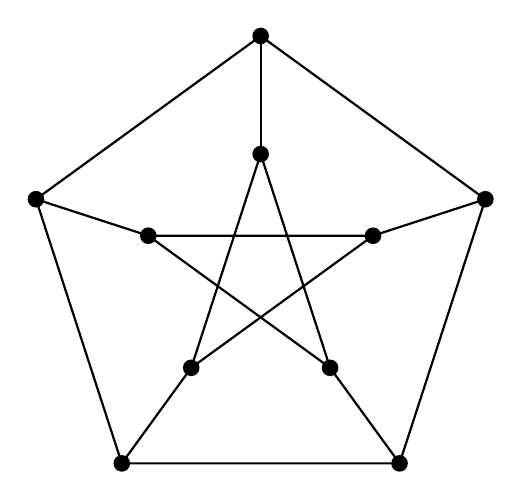
\begin{tikzpicture}[scale=1.5, auto, swap]
            % A simple nice Petersen graph or similar schematic to match style
            \foreach \i in {1,...,5}
            \coordinate (o\i) at (90+72*\i:2);
            \foreach \i in {1,...,5}
            \coordinate (i\i) at (90+72*\i:1);
            
            \draw[thick] (o1) -- (o2) -- (o3) -- (o4) -- (o5) -- cycle;
            \draw[thick] (i1) -- (i3) -- (i5) -- (i2) -- (i4) -- cycle;
            \foreach \i in {1,...,5} \draw[thick] (o\i) -- (i\i);
            
            \foreach \i in {1,...,5} \fill (o\i) circle (2pt);
            \foreach \i in {1,...,5} \fill (i\i) circle (2pt);
        \end{tikzpicture}
        \\[2.5cm]
        
        \begin{minipage}{0.4\textwidth}
            \begin{flushleft} \large
                \emph{Lecturer:}\\
                Isabel Müller
            \end{flushleft}
        \end{minipage}
        \begin{minipage}{0.4\textwidth}
            \begin{flushright} \large
                \emph{Term:} \\
                Spring 2026
            \end{flushright}
        \end{minipage}
        
    \end{center}
\end{titlepage}

% =============================================================
% DEDICATION (German)
% =============================================================
\newpage
\thispagestyle{empty}
\vspace*{\fill}
\begin{center}
    \textit{\Large "An die Professorin, der ich meine Wertschätzung nicht zeigen konnte,\\ und an die Professorin, der ich es niemals vergelten kann."}
\end{center}
\vspace*{\fill}
\newpage

% =============================================================
% TABLE OF CONTENTS
% =============================================================
\tableofcontents
\newpage

% =============================================================
% CHAPTERS
% =============================================================

% We will uncomment these as we create them
% !TEX root = main.tex

\chapter{Graphs}
\section{The Basics}

\subsection{Recall}

\begin{definition}{Set}
A \textbf{set} is merely an accumulation of objects. These objects are called \textbf{elements} of the set. If an object $x$ is an element of $S$, we write $x \in S$. The set of all elements with a certain property $P$ is denoted via $\{x \mid x \text{ has property } P\}$.
\end{definition}

\begin{definition}{Relation}
An \textbf{$n$-ary relation} $R$ on a set $A$ is a subset of the power set of $A^n$, i.e., $R \subseteq \mathcal{P}(A^n)$. If $n=2$, we call the relation \textbf{binary}.
\end{definition}

A binary relation $R$ on a set $A$ is called:
\begin{itemize}
    \item[(i)] \textbf{symmetric} if $R(a,b)$ implies $R(b,a)$ for all $a,b \in A$.
    \item[(ii)] \textbf{asymmetric} if $R(a,b)$ implies $\neg R(b,a)$ for all $a,b \in A$.
    \item[(iii)] \textbf{antisymmetric} if $R(a,b) \land R(b,a)$ implies $a=b$ for all $a,b \in A$.
    \item[(iv)] \textbf{reflexive} if $R(a,a)$ for all $a \in A$.
    \item[(v)] \textbf{irreflexive} if $\neg R(a,a)$ for all $a \in A$.
    \item[(vi)] \textbf{transitive} if $R(a,b) \land R(b,c)$ implies $R(a,c)$ for all $a,b,c \in A$.
\end{itemize}

\subsection{Definition of a Graph}

\begin{definition}{Graph}
A \textbf{graph} $G=(V,E)$ is a pair of sets $V$ and $E$ s.t. $E$ consists of subsets of $V$ of size two. $V$ is called the set of \textbf{vertices} and $E$ the set of \textbf{edges}. A graph $G$ is called \textbf{finite} if $V$ is a finite set. The \textbf{order} $|G|$ of a graph $G=(V,E)$ is the cardinality of its vertex set, so $|G|=|V|$. The \textbf{size} $\|G\|$ of $G$ is the cardinality of its edge set, $\|G\|=|E|$.
\end{definition}

\subsection{Visualisation}

Let $G=(V,E)$ be a graph. We visualise vertices $u,v \dots \in V$ by dots and edges $e=\{u,v\} \in E$ by the diagram:

\begin{center}
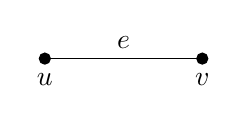
\begin{tikzpicture}
    \filldraw (0,0) circle (2pt) node[below=2pt] {$u$};
    \filldraw (2,0) circle (2pt) node[below=2pt] {$v$};
    \draw (0,0) -- (2,0) node[midway, above] {$e$};
\end{tikzpicture}
\end{center}

\begin{example}[Bowtie Graph]
Let $G=(V,E)$ be the graph with $V=\{a,b,c,d,e\}$ and
\[ E = \{\{a,b\}, \{a,c\}, \{a,d\}, \{a,e\}, \{b,c\}, \{d,e\}\}. \]
The graph $G$ has order 5 and size 6. It can be visualized via:
\begin{center}
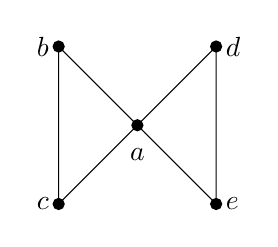
\begin{tikzpicture}
    \coordinate (a) at (0,0);
    \coordinate (b) at (-1,1);
    \coordinate (c) at (-1,-1);
    \coordinate (d) at (1,1);
    \coordinate (e) at (1,-1);

    \draw (b) -- (a) -- (c) -- (b);
    \draw (d) -- (a) -- (e) -- (d);

    \filldraw (a) circle (2pt) node[below=5pt] {$a$};
    \filldraw (b) circle (2pt) node[left] {$b$};
    \filldraw (c) circle (2pt) node[left] {$c$};
    \filldraw (d) circle (2pt) node[right] {$d$};
    \filldraw (e) circle (2pt) node[right] {$e$};
\end{tikzpicture}
\end{center}
This visualisation motivates its name: \textbf{bowtie graph}.
\end{example}

\subsection{Notation}

\begin{enumerate}
    \item For a graph $G=(V,E)$ we may denote its vertex set by $V(G)$ or $V_G$ for clarity.
    \item Similarly, we often denote $E$ by $E(G)$ or $E_G$.
    \item We denote an edge $\{u,v\}$ simply by $uv$.
    \item Edges are often called $e, e_1, e_2, f \dots$, while vertices are called $u, v, x, y, \dots$.
\end{enumerate}

\subsection{Terminology}

\begin{definition}{Adjacency and Incidence}
Let $G=(V,E)$ be a graph.
\begin{enumerate}
    \item If $uv \in E$ is an edge, then we say that $u$ and $v$ are \textbf{adjacent} or \textbf{neighbours}. If $uv \notin E$, we call $u$ and $v$ \textbf{nonadjacent}.
    \item If $e=uv \in E$, we say that $u$ and $v$ are the \textbf{end vertices} of $e$ or that they are \textbf{incident} with $e$.
    \item The \textbf{neighborhood} $N(v)$ of a vertex $v \in V$ is the set of all vertices adjacent to $v$, i.e., $N(v) = \{u \in V \mid uv \in E\}$. The \textbf{closed neighborhood} $N[v]$ of $v$ is $N[v] := N(v) \cup \{v\}$.
    \item The \textbf{neighborhood} $N(S)$ of a set of vertices is defined as $N(S) := \bigcup_{v \in S} N(v)$. Similarly, the \textbf{closed neighborhood} $N[S]$ is set to be $N[S] := N(S) \cup S (= \bigcup_{v \in S} N[v])$.
    \item The \textbf{degree} $\deg(v)$ of $v \in V$ is the number of edges incident with $v$, i.e., $\deg(v) := |\{e \in E \mid v \in e\}| = |N(v)|$.
    \item The \textbf{maximum degree} $\Delta(G)$ of $G$ is defined as
    \[ \Delta(G) := \max \{ \deg(v) \mid v \in V \}. \]
    Similarly, $\delta(G) := \min \{ \deg(v) \mid v \in V \}$ is the \textbf{minimum degree} of $G$.
    \item The \textbf{degree sequence} of a graph $G$ is the sequence containing all degrees of the vertices of $G$ (with repetition) in decreasing order.
\end{enumerate}
\end{definition}

\begin{example}
Consider $G$ given by:
\begin{center}
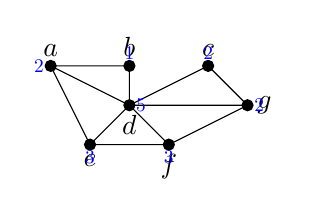
\begin{tikzpicture}
    \coordinate (a) at (0,1);
    \coordinate (b) at (1,1);
    \coordinate (c) at (2,1);
    \coordinate (d) at (1,0.5);
    \coordinate (e) at (0.5,0);
    \coordinate (f) at (1.5,0);
    \coordinate (g) at (2.5,0.5);

    \draw (a) -- (d) -- (b) -- (a) -- (e) -- (d) -- (f) -- (e);
    \draw (d) -- (g) -- (c) -- (d);
    \draw (f) -- (g);

    \foreach \point in {a,b,c,d,e,f,g} \filldraw (\point) circle (2pt);
    \node[above] at (a) {$a$}; \node[above] at (b) {$b$}; \node[above] at (c) {$c$};
    \node[below] at (d) {$d$}; \node[below] at (e) {$e$}; \node[below] at (f) {$f$}; \node[right] at (g) {$g$};
    
    % Degree annotations (small)
    \node[left, blue, scale=0.7] at (a) {2};
    \node[above, blue, scale=0.7] at (b) {1};
    \node[above, blue, scale=0.7] at (c) {2};
    \node[right, blue, scale=0.7] at (g) {2};
    \node[below, blue, scale=0.7] at (f) {3};
    \node[below, blue, scale=0.7] at (e) {3};
    \node[right, blue, scale=0.7] at (d) {5};
\end{tikzpicture}
\end{center}
Then $\Delta(G)=5$, $\delta(G)=1$. $N(e)=\{a,d,f\}$, $N[b]=\{b,d\}$, $N[\{a,g\}]=\{a,c,d,e,f,g\}$.
Order of $G$ is 7, size of $G$ is 9. Degree sequence is $(5,3,3,2,2,2,1)$.
\end{example}

\begin{remark}
A graph can be considered as a set $V$ together with a binary relation $E$ on $V$ which is symmetric and irreflexive.
\end{remark}

\subsection{Handshaking Lemma}

\begin{theorem}{The Handshaking Lemma}
If $G=(V,E)$ is a graph, then
\[ \sum_{v \in V} \deg(v) = 2|E|. \]
\end{theorem}

\begin{proof}
We proceed by induction on $n := |E|$.
\textbf{n=0:} If $|E|=0$, then $\deg(v)=0$ for any $v \in V$, whence clearly $0 = \sum \deg(v) = 2|E| = 0$.

\textbf{n $\to$ n+1:} Assume $(*)$ holds for any $G'=(V',E')$ with $|E'|=n$ (I.H.) and consider $G=(V,E)$ with $|E|=n+1 (\ge 1)$ arbitrary. Let $e \in E$ arbitrary and consider $G'=(V, E \setminus \{e\})$. Then, if $e=uv$, we get $|E(G)| = |E(G')|+1$ and
\[ \deg_G(u) = \deg_{G'}(u) + 1 \quad \text{and} \quad \deg_G(v) = \deg_{G'}(v) + 1, \]
whence
\[ 2|E(G)| = 2|E(G')| + 2 \overset{\text{I.H.}}{=} \sum_{w \in V} \deg_{G'}(w) + 2 \]
\[ = \sum_{w \in V \setminus \{u,v\}} \deg_{G'}(w) + \deg_{G'}(u) + 1 + \deg_{G'}(v) + 1 \]
\[ = \sum_{w \in V} \deg_G(w), \text{ as desired.} \qedhere \]
\end{proof}

\begin{corollary}{Odd Degrees}
Any graph $G$ has an even number of vertices of odd degree.
\end{corollary}
\begin{proof}
Exercise.
\end{proof}

\begin{corollary}{Bounds}
For any graph $G=(V,E)$ we have
\[ \delta(G) \le 2 \frac{|E|}{|V|} \le \Delta(G). \]
\end{corollary}
\begin{proof}
\[ |V| \cdot \delta(G) = \sum_{v \in V} \delta(G) \le \sum_{v \in V} \deg(v) \le \sum_{v \in V} \Delta(G) = |V|\Delta(G) \]
Using Theorem 1.13, $\sum \deg(v) = 2|E|$. Dividing by $|V|$ yields the result.
\end{proof}

\begin{lemma}{Pigeon Hole Principle for Graphs}
If $|G| \ge 2$, then $G$ contains at least two vertices of the same degree.
\end{lemma}
\begin{proof}
If $G$ has two vertices of degree 0, then we are done. Otherwise, we may assume that $G$ has none. If $|V|=n$, and $v \in V$, then $1 \le \deg(v) \le n-1$. Note that this leaves us with $n-1$ choices of degrees for $n$ many different vertices. Hence, at least two vertices must have the same degree.
\end{proof}

\begin{remark}
The above line of thought is called the \textbf{pigeon hole principle}. If there are $n$ many pigeons wanting to fit into $n-1$ many holes, then at least two of them have to cuddle up in the same hole.
\end{remark}

\subsection{Special Graphs}

\begin{definition}{Paths, Cycles, Complements}
\begin{enumerate}
    \item The \textbf{path} $P_n$ is the graph on $n$ vertices $v_1, \dots, v_n$ with the edge set $E(P_n) = \{v_i v_{i+1} \mid 1 \le i < n\}$.
    \item The \textbf{cycle} $C_n$ is the graph on $n$ vertices with edge set $E(C_n) = \{v_i v_{i+1} \mid 1 \le i < n\} \cup \{v_n v_1\}$.
    \item Let $G=(V,E)$ be an arbitrary graph. The \textbf{complement} $\overline{G}$ of $G$ is the graph $\overline{G}=(V, \overline{E})$, where $\overline{E} = \{uv \mid u,v \in V, uv \notin E\}$.
\end{enumerate}
\end{definition}

\begin{definition}{Regularity}
We call a graph $G$ \textbf{regular} if any of its vertices has the same degree. If this degree is $r$, we say that $G$ is \textbf{$r$-regular}.
\end{definition}

\begin{definition}{Complete Graph}
The \textbf{complete graph} $K_n$ for $n \ge 1$ is the graph consisting of $n$ vertices such that any two vertices are adjacent. The \textbf{empty graph} $E_n$ is the graph consisting of $n$ vertices and no edges.
\end{definition}

\subsection{Subgraphs}

\begin{definition}{Subgraphs}
\begin{enumerate}
    \item A graph $H$ is called a \textbf{subgraph} of some graph $G$, written $H \subseteq G$, if $V(H) \subseteq V(G)$ and $E(H) \subseteq E(G)$.
    \item If $H \subseteq G$, we say that $H$ is an \textbf{induced subgraph} of $G$, written $H \sqsubseteq G$, if $E(H) = \{uv \in E(G) \mid u,v \in V(H)\}$.
\end{enumerate}
\end{definition}

\begin{remark}
If $G$ is a graph and $S \subseteq V(G)$, then there is only one induced subgraph $H \sqsubseteq G$ with vertex set $S$. We denote this graph by $\langle S \rangle$ and call it the subgraph of $G$ induced by $S$.
\end{remark}

\subsection{Walks in Graphs}

\begin{definition}{Walk}
A $(v_0, v_k)$-\textbf{walk} in a graph is a sequence of vertices $(v_0, v_1, \dots, v_k)$ s.t. any two consecutive vertices $v_i$ and $v_{i+1}$ are adjacent. We call the edges $\{v_0v_1, v_1v_2, \dots, v_{k-1}v_k\}$ the \textbf{edges of the walk}. We say that the walk is \textbf{closed} if $v_0=v_k$. The \textbf{length} of a walk is the number of edges in it (counting repetition).
\end{definition}

\begin{definition}{Types of Walks}
We distinguish the following types of walks:
\begin{itemize}
    \item A \textbf{trail} is a walk whose edges are pairwise distinct.
    \item A \textbf{circuit} is a closed walk whose edges are pairwise distinct.
    \item A \textbf{path} is a walk whose vertices are distinct.
    \item A \textbf{cycle} is a closed walk $(v_0, \dots, v_k=v_0)$ with $k \ge 3$ and whose vertices $v_0, \dots, v_{k-1}$ are pairwise distinct.
\end{itemize}
\end{definition}

\begin{lemma}{Cycle Existence}
If $\delta(G) \ge 2$, then $G$ contains a cycle as a subgraph.
\end{lemma}
\begin{proof}
Let $P = (v_0, \dots, v_k)$ be a path in $G$ of maximal length. This exists, as $G$ is finite. Further, as $\delta(G) \ge 2$, we get $k \ge 2$. As $\deg(v_0) \ge \delta(G) \ge 2$, $v_0$ has at least two neighbors. One of them is $v_1$. Let us denote the other one by $u$. If $u \ne v_i$ for all $1 \le i \le k$, then $\tilde{P} = (u, v_0, v_1, \dots, v_k)$ is still a path and of greater length than $P$, contradicting our assumptions. Hence, $u=v_i$ for some $1 \le i \le k$. But then the sequence $(v_0, v_1, \dots, v_i=u, v_0)$ is the desired cycle subgraph of $G$.
\end{proof}

\begin{theorem}{Walk-Path Theorem}
Every $uv$-walk in a graph contains a $uv$-path.
\end{theorem}
\begin{proof}
We proceed by strong induction on the length $n \ge 1$ of the walk.
\textbf{I.B. n=1.} If the $uv$-walk is of length one, then it is exactly $(u,v)$, which is also a path.
\textbf{I.S.} Assume every $uv$-walk of length at most $n \ge 1$ contains a $uv$-path (I.H.). Assume there is a $uv$-walk $W=(u=w_0, w_1, \dots, w_n, w_{n+1}=v)$ of length $n+1$. If $W$ is already a path, we are done. Otherwise there are $i,j$ s.t. $0 \le i < j \le n+1$ and $w_i = w_j$. But then the walk $\tilde{W}$ which arises from $W$ by deleting the vertices $w_{i+1}, \dots, w_{j-1}, w_j$, i.e. $\tilde{W} = (u=w_0, \dots, w_i, w_{j+1}, \dots, w_{n+1}=v)$ is still a $uv$-walk, but of length at most $n$. Using I.H., we know that $\tilde{W}$ contains a $uv$-path, whence also $W$ contains (the same) $uv$-path.
\end{proof}

\subsection{Connectivity}

\begin{definition}{Connected}
A graph is \textbf{connected} if there exists an $uv$-path in $G$ for any vertices $u,v \in V(G)$. Otherwise, it is called \textbf{disconnected}.
\end{definition}

\begin{definition}{Connected Component}
A \textbf{connected component} of $G$ is a maximal connected induced subgraph of $G$. i.e. $C \sqsubseteq G$ is a connected component iff (i) $C$ is connected and (ii) for any $v \in V(G) \setminus V(C)$ the induced subgraph on $V(C) \cup \{v\}$ is \textbf{not} connected.
\end{definition}

\begin{remark}
$G$ is connected iff it has exactly one connected component. Even among connected graphs, there are different levels of being connected. E.g. the graph $K_5$ "feels" more connected than the graph consisting of two triangles joined by a single edge.
\end{remark}

\begin{definition}{Deletion}
Let $G$ be a graph, $S \subseteq V_G$ and $T \subseteq E_G$.
\begin{enumerate}
    \item By $G-S$ we denote the graph arising from $G$ by removing from $V_G$ all vertices in $S$ and their incident edges.
    \item If $S=\{v\}$, we write $G-v$.
    \item By $G-T$ we denote the graph arising from $G$ by removing only the edges in $T$, but no vertices.
    \item If $T=\{e\}$, we write $G-e$.
\end{enumerate}
\end{definition}

\begin{definition}{Cut Vertex and Bridge}
Let $G$ be a graph.
\begin{enumerate}
    \item We call $v \in V_G$ a \textbf{cut vertex} if $G-v$ has more connected components than $G$ itself.
    \item We call $e \in E_G$ a \textbf{bridge} if $G-e$ has more connected components than $G$ itself.
    \item We call $S \subseteq V_G$ a \textbf{cut set} if $G-S$ is disconnected.
    \item A connected graph which does not contain any cut vertices is called \textbf{non-separable}.
\end{enumerate}
\end{definition}

\begin{definition}{Connectivity}
For a non-complete graph $G$, we define its \textbf{connectivity} $\kappa(G)$ as the minimal size of a cut set. For $K_n$, we set $\kappa(K_n) = n-1$.
We say that $G$ is \textbf{$k$-connected} if $\kappa(G) \ge k$, i.e. if $G$ is connected and $G-S$ is still connected for any $S \subseteq V_G$ with $|S| < k$.
\end{definition}

\begin{lemma}{Properties of Connectivity}
The following hold:
\begin{enumerate}
    \item $G$ is connected iff $\kappa(G) \ge 1$.
    \item $G$ is 2-connected iff $G$ is connected and has no cut vertices.
    \item $|G| > \kappa(G)$.
    \item $\kappa(G) \le \delta(G)$.
\end{enumerate}
\end{lemma}

\begin{proof}
4) Assume $\kappa(G) > \delta(G)$ and let $v \in V_G$ s.t. $\deg(v)=\delta(G)$. Note that $|G| > \kappa(G) > \delta(G) = |N(v)|$, whence $G-N(v)$ contains at least one vertex besides $v$. But clearly, $G-N(v)$ is disconnected (as $\deg_{G-N(v)}(v)=0$). Hence, $N(v)$ is a cut set and $\kappa(G) \le |N(v)| = \delta(G)$, contradicting the assumptions.
\end{proof}

\section{Bipartite Graphs}

\begin{definition}{Bipartite}
A graph $G$ is called \textbf{bipartite} if we can partition the vertex set $V_G$ into two disjoint sets $V_G = X \cup Y$ s.t. every edge of $G$ has one end vertex in $X$ and the other in $Y$.
\end{definition}

\begin{remark}
A graph $G$ is bipartite if and only if we can color the vertices of $G$ with two colors s.t. the end vertices of each edge have different colors.
\end{remark}

\begin{definition}{Complete Bipartite}
Let $m,n \in \mathbb{Z}_+$. The \textbf{complete bipartite graph} $K_{m,n}$ is the bipartite graph with $X=\{x_1, \dots, x_m\}$, $Y=\{y_1, \dots, y_n\}$, $V_G=X \cup Y$ and $E_G = \{xy \mid x \in X, y \in Y\}$.
\end{definition}

\begin{theorem}{Characterization of Bipartite Graphs}
A graph is bipartite iff it does not contain odd cycles.
\end{theorem}

\begin{proof}
"$\Rightarrow$": Assume $G$ is bipartite and nevertheless there is a cycle of odd length, say $(x_0, x_1, \dots, x_{2k}, x_{2k+1}=x_0)$. By Remark 1.44, we can color $V_G$ in two colors, $C1$ and $C2$. If $x_0$ has color $C1$, $x_1$ has color $C2$, whence $x_2$ has color $C1$. That way we see that the color of $x_i$ is $C1$ if $i$ is even and $C2$ if $i$ is odd. Following that logic, $x_{2k+1}$ should have color $C2$, but $x_{2k+1}=x_0$ has color $C1$, a contradiction.

"$\Leftarrow$": Now consider that $G$ does not contain odd cycles. We will show that $G$ is bipartite by providing a partition. We may assume that $G$ is connected as otherwise we work component per component.
Pick $v \in V_G$ arbitrary and define
\[ X = \{w \in V_G \mid \text{the shortest } vw \text{ path has even length}\} \]
\[ Y = \{w \in V_G \mid \text{the shortest } vw \text{ path has odd length}\}. \]
Clearly $X$ and $Y$ are disjoint. We will show that there are no adjacent vertices in $X$ or $Y$ respectively. Note that $v \in X$.
Aiming for a contradiction, assume there are vertices $w_1, w_2 \in X$ which are adjacent. Let $P_1$ and $P_2$ be the shortest $v-w_1$ and $v-w_2$ paths.
We construct a cycle using $P_1$, the edge $w_1w_2$, and $P_2$. The length of this cycle is $len(P_1) + 1 + len(P_2) = \text{even} + 1 + \text{even} = \text{odd}$. This contradicts our assumption.
\end{proof}

\section{Graph Isomorphisms}

\begin{definition}{Isomorphism}
We say that a graph $G$ is \textbf{isomorphic} to a graph $H$ if there exists a bijection $\varphi: V_G \to V_H$ s.t. for any $u,v \in V_G$ we have that $\{u,v\} \in E_G$ if and only if $\{\varphi(u), \varphi(v)\} \in E_H$. Then, the map $\varphi$ is called an \textbf{isomorphism} and we write $G \cong H$.
\end{definition}

\begin{remark}
Let $G \cong H$ via $\varphi: V_G \to V_H$. Then:
\begin{enumerate}
    \item $|V_G|=|V_H|$ and $|E_G|=|E_H|$.
    \item The degree sequence of $G$ equals the degree sequence of $H$.
    \item $G$ is connected iff $H$ is connected.
    \item $\deg_G(v) = \deg_H(\varphi(v))$ for all $v \in V_G$.
\end{enumerate}
\end{remark}
\chapter{Distance in Graphs}

\section{introduction}

We have a natural understanding of the ``distance'' between two objects in our physical space. But there are many other ways of defining distances. E.g., the distance between people could be the positive difference of their birth years or the number of acquaintances you need to connect one to the other.

In this chapter we will introduce a notion of distance of vertices in a graph. But first let us note what are the characterising properties that make us call all these concepts ``distances''.

% 2.1 Definition
\begin{definition}
Let $X$ be any set. We call a function $d: X \times X \to \mathbb{R}^{\ge 0} \cup \{\infty\}$ a \textbf{\color{red}metric} if it satisfies for all $x,y,z \in X$:
\begin{enumerate}
    \item[1)] $d(x,y) \ge 0$
    \item[2)] $d(x,y) = 0$ iff $x=y$
    \item[3)] $d(x,y) = d(y,x)$
    \item[4)] $d(x,z) \le d(x,y) + d(y,z)$ (\textbf{\color{red}Triangle Inequality})
\end{enumerate}
We then call the pair $(X,d)$ a \textbf{\color{red}metric space}.
\begin{center}
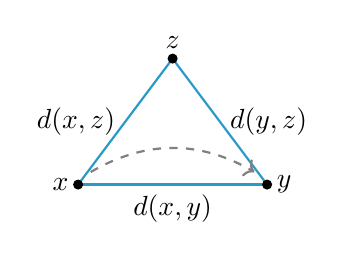
\begin{tikzpicture}[scale=0.8]
    \coordinate (x) at (0,0);
    \coordinate (y) at (3,0);
    \coordinate (z) at (1.5, 2);
    
    \draw[cyan!80!black, thick] (x) -- (y) node[midway, below, black] {$d(x,y)$};
    \draw[cyan!80!black, thick] (x) -- (z) node[midway, left, black] {$d(x,z)$};
    \draw[cyan!80!black, thick] (z) -- (y) node[midway, right, black] {$d(y,z)$};
    
    \filldraw (x) circle (2pt) node[left] {$x$};
    \filldraw (y) circle (2pt) node[right] {$y$};
    \filldraw (z) circle (2pt) node[above] {$z$};
    
    % Visualizing triangle inequality shortcut
    \draw[->, gray, dashed, thick] (0.2, 0.2) to[bend left] (2.8, 0.2);
\end{tikzpicture}
\end{center}
\end{definition}

% 2.2 Example
\begin{example}
Consider $X=\mathbb{R}$ and $d: \mathbb{R} \times \mathbb{R} \to \mathbb{R}^{\ge 0}$ via $d(x,y) := |x-y|$. Then $(\mathbb{R}, d)$ is a metric space.
\end{example}

Now we are ready to define a metric on an arbitrary graph.

% 2.3 Definition
\begin{definition}
Let $G$ be any graph and $u,v \in V_G$. We define the \textbf{\color{red}distance $d(u,v)$} between $u$ and $v$ as the length of the shortest $uv$-path in $G$, i.e.
\[ d(u,v) := \min \{ \text{length}(P) \mid P \text{ is a } uv\text{-path} \}. \]
If there is no such path, we set \textbf{\color{red}$d(u,v) := \infty$}.

2) If $d(u,v)=k$, then any $uv$-path of length $k$ is called a \textbf{\color{red}geodesic}.
\end{definition}

% 2.4 Remark
\begin{remark}
\begin{enumerate}
    \item[1)] We may write $d_G(u,v)$ to emphasize that we consider the distance in $G$.
    \item[2)] While in $(\mathbb{R}, d)$ geodesics are unique, in general this is not the case. Consider for example two opposite poles on a sphere.
    \item[3)] $d(x,y)=\infty$ iff $x$ and $y$ are in different connected components.
    \item[4)] $(V_G, d)$ is a metric space for any connected graph $G$.
\end{enumerate}
\end{remark}

We call something eccentric if it is away from the usual. Similarly, in graphs we measure by eccentricity how far a vertex is from the center. Consider the following notions on a cycle:

\begin{center}
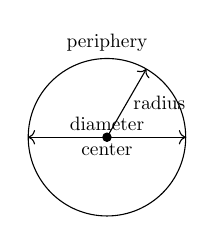
\begin{tikzpicture}
    \draw (0,0) circle (1cm);
    \filldraw (0,0) circle (1.5pt) node[below, scale=0.7] {center};
    \draw[->] (0,0) -- (60:1) node[midway, right, scale=0.7] {radius};
    \draw[<->] (-1,0) -- (1,0) node[midway, above, scale=0.7] {diameter};
    \node[scale=0.7] at (0, 1.2) {periphery};
\end{tikzpicture}
\end{center}

% 2.5 Definition
\begin{definition}
\begin{enumerate}
    \item[1)] The \textbf{\color{red}eccentricity $ecc(v)$} of a vertex $v$ is its greatest distance to any other vertex, i.e. $ecc(v) = \max \{ d(u,v) \mid u \in V_G \}$.
    \item[2)] The \textbf{\color{red}radius $rad(G)$} is the smallest possible eccentricity and the \textbf{\color{red}diameter $diam(G)$} is the largest possible eccentricity.
    \item[3)] The \textbf{\color{red}center $C(G)$} is the set $\{v \in V_G \mid ecc(v) = rad(G)\}$ and the \textbf{\color{red}periphery $P(G)$} is the set $\{v \in V_G \mid ecc(v) = diam(G)\}$.
\end{enumerate}
\end{definition}

% 2.6 Example
\begin{example}
1) Consider $P_5$, the path of length 4, i.e.
\begin{center}
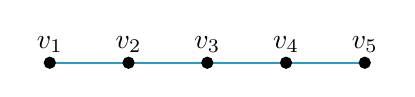
\begin{tikzpicture}
    \draw[cyan!80!black, thick] (0,0) -- (4,0);
    \foreach \i in {1,...,5} \filldraw (\i-1, 0) circle (2pt) node[above] {$v_\i$};
\end{tikzpicture}
\end{center}
Then
\begin{align*}
    d(v_1, v_i) &= i-1, \text{ whence } ecc(v_1) = \max\{0,1,2,3,4\} = 4. \\
    d(v_2, v_i) &= |i-2|, \text{ whence } ecc(v_2) = \max\{1,0,1,2,3\} = 3. \\
    d(v_3, v_i) &= |i-3|, \text{ whence } ecc(v_3) = \max\{2,1,0,1,2\} = 2. \\
    d(v_4, v_i) &= |i-4|, \text{ whence } ecc(v_4) = \max\{3,2,1,0,1\} = 3. \\
    d(v_5, v_i) &= |i-5|, \text{ whence } ecc(v_5) = \max\{4,3,2,1,0\} = 4.
\end{align*}
Hence $rad(P_5) = \min\{ecc(v) \mid v \in V\} = \min\{4,3,2,3,4\} = 2$.
Also $C(P_5) = \{v \in V \mid ecc(v) = rad(P_5)\} = \{v_3\}$.
Further $diam(P_5) = \max\{ecc(v) \mid v \in V\} = \max\{4,3,2,3,4\} = 4$.
And $P(P_5) = \{v \in V \mid ecc(v) = diam(P_5)\} = \{v_1, v_5\}$.

2) Consider $G := C_6$, the cycle of length 6, i.e. $G=$
\begin{center}
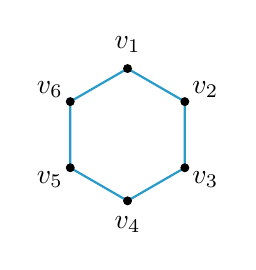
\begin{tikzpicture}[scale=0.7, baseline=(current bounding box.center)]
    \foreach \i in {1,...,6} \coordinate (v\i) at (90+60-60*\i : 1.2);
    \draw[cyan!80!black, thick] (v1)--(v2)--(v3)--(v4)--(v5)--(v6)--(v1);
    \foreach \i in {1,...,6} \filldraw (v\i) circle (2pt) node[anchor=center, shift={(90+60-60*\i:0.3)}] {$v_\i$};
\end{tikzpicture}
\end{center}
Then $d(v_0, v_i)$... (calculations symmetric).
$ecc(v_0) = \max\{0,1,2,3,2,1\} = 3$.
Actually $ecc(v) = 3$ for all $v$.
Hence, $rad(G) = \min\{3,3,3,3,3,3\} = 3$.
Whence $C(G) = V_G$.
Further, $diam(G) = \max\{3,3,3,3,3,3\} = 3$.
And $P(G) = V_G$.
\end{example}

\topic{Intermezzo}

I: Find $rad(G), diam(G), C(G)$ and $P(G)$ of the following:
1) $G_1 = P_{10}$ \hspace{1cm} 2) $G_2 = K_6$

II: Consider
\begin{center}
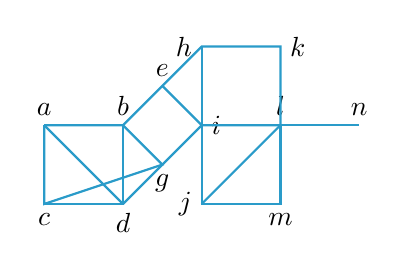
\begin{tikzpicture}
    % Graph from Intermezzo
    \coordinate (a) at (0,1); \node[above] at (a) {$a$};
    \coordinate (b) at (1,1); \node[above] at (b) {$b$};
    \coordinate (e) at (1.5, 1.5); \node[above] at (e) {$e$};
    \coordinate (h) at (2, 2); \node[left] at (h) {$h$};
    \coordinate (k) at (3, 2); \node[right] at (k) {$k$};
    \coordinate (i) at (2, 1); \node[right] at (i) {$i$};
    \coordinate (l) at (3, 1); \node[above] at (l) {$l$};
    \coordinate (n) at (4, 1); \node[above] at (n) {$n$};
    \coordinate (f) at (1.5, 0.5); \node[below] at (f) {$g$}; % Wait, note says g below f
    \coordinate (c) at (0,0); \node[below] at (c) {$c$};
    \coordinate (d) at (1,0); \node[below] at (d) {$d$};
    \coordinate (j) at (2,0); \node[left] at (j) {$j$};
    \coordinate (m) at (3,0); \node[below] at (m) {$m$};
    
    % Draw left square
    \draw[cyan!80!black, thick] (a)--(b)--(f)--(c)--(a); 
    \draw[cyan!80!black, thick] (c)--(d)--(b); % Cross in square
    \draw[cyan!80!black, thick] (a)--(d); % Cross
    \draw[cyan!80!black, thick] (f)--(d);
    
    % Connection to right part
    \draw[cyan!80!black, thick] (b)--(e)--(h)--(k)--(l)--(i)--(e);
    \draw[cyan!80!black, thick] (h)--(i); % vertical? No
    \draw[cyan!80!black, thick] (f)--(i);
    \draw[cyan!80!black, thick] (i)--(j)--(m)--(l)--(n);
    \draw[cyan!80!black, thick] (j)--(l);
    
    % Let's approximate the sketch better based on standard Intermezzo style
    % It looks like two house/square shapes connected.
    % I will draw a representative graph based on the nodes shown.
\end{tikzpicture}
\end{center}
Find:
\begin{itemize}
    \item $d(b,c), d(h,k), d(a,m)$
    \item $ecc(v)$ for all $v \in V_G$
    \item $rad(G), diam(G), C(G), P(G)$.
\end{itemize}

% 2.7 Lemma
\begin{lemma}
For any graph $G$ we have $rad(G) \le diam(G) \le 2 rad(G)$.
\end{lemma}

\begin{proof}
We have $rad(G) \le diam(G)$ by definition. For the other inequality, pick $v \in C(G)$ arbitrary and consider $u,w \in V_G$ arbitrary s.t. $d(u,w) = diam(G)$. Then
\[ d(u,w) \le d(u,v) + d(v,w) \le ecc(v) + ecc(v) = 2 rad(G). \qedhere \]
\end{proof}

% 2.8 Theorem
\begin{theorem}
Every graph $G$ is isomorphic to the graph induced by the center of another graph $H$, i.e. ex. $H$ s.t. $G \cong \langle C(H) \rangle$.
\end{theorem}

\begin{proof}
Let $G$ be arbitrary. We build a new graph $H$ which contains $G$ as an induced subgraph via: $V_H = V_G \cup \{u,x,y,z\}$, i.e. adding 4 new vertices to $G$. Further, let $E_H = E_G \cup \{ux, yz\} \cup \{xv, vy \mid v \in V_G\}$.

\begin{center}
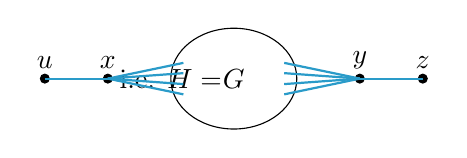
\begin{tikzpicture}[scale=0.8]
    \node at (-1,0) {i.e. $H=$};
    \draw (0,0) ellipse (1cm and 0.8cm); \node at (0,0) {$G$};
    
    \coordinate (x) at (-2,0); \filldraw (x) circle (2pt) node[above] {$x$};
    \coordinate (y) at (2,0); \filldraw (y) circle (2pt) node[above] {$y$};
    \coordinate (u) at (-3,0); \filldraw (u) circle (2pt) node[above] {$u$};
    \coordinate (z) at (3,0); \filldraw (z) circle (2pt) node[above] {$z$};
    
    \draw[cyan!80!black, thick] (u)--(x);
    \draw[cyan!80!black, thick] (y)--(z);
    
    % Connections to G
    \foreach \ang in {150, 170, 190, 210} \draw[cyan!80!black, thick] (x) -- (-0.8, {0.5*sin(\ang)});
    \foreach \ang in {-30, -10, 10, 30} \draw[cyan!80!black, thick] (y) -- (0.8, {0.5*sin(\ang)});
\end{tikzpicture}
\end{center}

Now $ecc(v)=2$ for any $v \in V_G$. Nevertheless, $d(u,z)=4$ and $d(x,z)=d(y,u)=3$, whence $ecc(w)>2$ for all $w \in V_H \setminus V_G$. Thus, $rad(H)=2$ and $C(H)=V_G$, whence $\langle C(H) \rangle \cong G$.
\end{proof}

% 2.9 Lemma
\begin{lemma}
A graph $G$ is isomorphic to the graph induced by the periphery of another graph $H$ iff either every vertex has eccentricity 1 or no vertex does.
\end{lemma}

\begin{proof}
``$\Rightarrow$'' We use proof by contraposition. Assume ex. $u \in V_G$ s.t. $ecc(u)=1 < diam(G)$. In particular, $G \ne P(G)$. Now, aiming for a contradiction, assume ex. $H$ s.t. $G \le H$ and $P(H) = V_G$.
As $G \ne P(G)$, we know that $H \ne G$ and $diam(H) \ge 2$. As $u \in V_G = P(H)$, there is some $w \in V_H$ s.t. $d(u,w)=diam(H)$. But then, $w \in P(H) \cong V_G$, and as $ecc(u)=1$, we also get $d(u,w)=1 < diam(H)$. Hence, $P(H)$ cannot be $V_G$.

``$\Leftarrow$'' If all vertices in $G$ have eccentricity 1 or 0, then $G$ is complete and $G \cong P(G)$. For the second case, assume $rad(G)>1$. And consider $H$ s.t. $V_H = V_G \cup \{v\}$ contains one new vertex which is connected to everyone else, i.e. $E_H = E_G \cup \{vx \mid x \in V_G\}$. Then, as $ecc(x) \ge 2$ for all $x \in V_G$,
\[ ecc_H(x) = \begin{cases} 2 & \text{if } x \in V_G \\ 1 & \text{if } x=v \end{cases}. \]
Hence, $diam(H)=2$ and $\langle P(H) \rangle = G$, as desired.
\end{proof}

\section{Adjacency Matrices}

We saw the visual benefits of studying graphs by their diagram. This is very useful to illustrate ideas and study small graphs. In applications on the other hand, when studying e.g. correlations of weather phenomena or social links, graphs tend to have thousands of vertices. Here, it is no longer practical to use neither the set- nor the diagram representation of graphs. The way computers store and analyze graphs is by using adjacency matrices.

% 2.10 Definition
\begin{definition}
Let $G$ be a graph of order $n$ with vertices $V_G = \{v_1, v_2, \dots, v_n\}$. The \textbf{\color{red}adjacency matrix} of $G$ is the matrix $A_G = (a_{ij}) \in M_{n \times n}$ defined via
\[ a_{ij} = \begin{cases} 1 & \text{if } v_i v_j \in E \\ 0 & \text{otherwise}. \end{cases} \]
We also write $A(i,j)$ for $a_{ij}$.
\end{definition}

% 2.11 Example
\begin{example}
Consider $G$ given by
\begin{center}
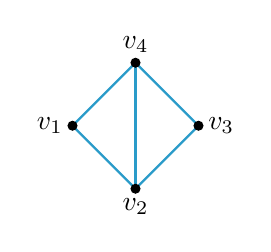
\begin{tikzpicture}[scale=0.8]
    \coordinate (v1) at (-1, 0); \node[left] at (v1) {$v_1$};
    \coordinate (v2) at (0, -1); \node[below] at (v2) {$v_2$};
    \coordinate (v3) at (1, 0); \node[right] at (v3) {$v_3$};
    \coordinate (v4) at (0, 1); \node[above] at (v4) {$v_4$};
    
    \draw[cyan!80!black, thick] (v1)--(v2)--(v3)--(v4)--(v1);
    \draw[cyan!80!black, thick] (v2)--(v4); % Cross
    
    \foreach \p in {v1,v2,v3,v4} \filldraw (\p) circle (2pt);
\end{tikzpicture}
\end{center}
Then $A_G \in M_{4 \times 4}$
\[ A_G = \begin{pmatrix} 0 & 1 & 0 & 1 \\ 1 & 0 & 1 & 1 \\ 0 & 1 & 0 & 1 \\ 1 & 1 & 1 & 0 \end{pmatrix} \]
is the adjacency matrix of $G$.
\end{example}

% 2.12 Remark
\begin{remark}
If $A_G = (a_{ij})$ is an adjacency matrix of a graph $G$, then
\begin{enumerate}
    \item[1)] $a_{ii} = 0$ for all $1 \le i \le |G|$
    \item[2)] $A$ is symmetric.
    \item[3)] $\sum_{j=1}^{|G|} a_{ij} = \deg(v_i)$ and thus $\sum_{i,j=1}^{|G|} a_{ij} = \sum_{i=1}^{|G|} \deg(v_i) = 2|E|$.
    \item[4)] $A_G$ is only unique up to reordering the vertices.
\end{enumerate}
\end{remark}

% 2.13 Example
\begin{example}
Let revisit the graph $G$ from 2.11. The fact that $A_G(2,3) \ne 0$ means that $v_2$ and $v_3$ are adjacent. And $A(1,3)=0$ says that $v_1$ and $v_3$ are not. Now consider
\[ A_G^2 = \begin{pmatrix} 0 & 1 & 0 & 1 \\ 1 & 0 & 1 & 1 \\ 0 & 1 & 0 & 1 \\ 1 & 1 & 1 & 0 \end{pmatrix} \begin{pmatrix} 0 & 1 & 0 & 1 \\ 1 & 0 & 1 & 1 \\ 0 & 1 & 0 & 1 \\ 1 & 1 & 1 & 0 \end{pmatrix} = \begin{pmatrix} 2 & 1 & 2 & 1 \\ 1 & 3 & 1 & 2 \\ 2 & 1 & 2 & 1 \\ 1 & 2 & 1 & 3 \end{pmatrix}. \]
Let's interpret the values of $A_G^2$.
Now, $A_G^2(1,3) = 2$. How did we compute it?
$A_G^2(1,3) = \sum_{j=1}^4 a_{1j} a_{j3}$. Now $a_{1j}a_{j3} = 1$ iff $v_1v_j$ and $v_j v_3$ are edges iff $(v_1, v_j, v_3)$ is a walk of length 2 from $v_1$ to $v_3$.
Hence, $A_G^2(1,3) = \sum a_{1j}a_{j3}$ is the number of walks from $v_1$ to $v_3$ of length 2. This generalises and provides a strong tool to study graphs.
\end{example}

% 2.14 Theorem
\begin{theorem}
Let $G$ be a graph with $V_G = \{v_1, \dots, v_n\}$ and $A_G$ the corresponding adjacency matrix. Then the entry $A_G^k(i,j)$ is the number of possible walks from $v_i$ to $v_j$ of length $k$.
\end{theorem}

\begin{proof}
We proceed by induction on the power $k$. (Note that $k=0$ works too).
\underline{$k=1$}: We get that $A(i,j) = \begin{cases} 0 & \text{iff } v_iv_j \notin E_G \text{ iff there are 0 } v_iv_j\text{-walks of length 1} \\ 1 & \text{iff } v_iv_j \in E_G \text{ iff there is 1 } v_iv_j\text{-walk of length 1} \end{cases}$.

\underline{$k \to k+1$}: Assume that $A^k(i,j)$ gives exactly the number of $v_iv_j$-walks of length exactly $k$. Let's denote $A^k = (b_{ij})$ and $A = (a_{ij})$.
Note that there is a $v_iv_j$-walk of length $k+1$ iff there ex. a vertex $v_\ell$ s.t. there is a $v_iv_\ell$-walk of length $k$ and an $v_\ell v_j$-walk of length one. Hence
\begin{align*}
    |\{v_iv_j\text{-walk of length } k+1\}| &= \sum_{\ell \mid v_\ell \in N(v_j)} |\{v_iv_\ell\text{-walk of length } k\}| \\
    &\overset{\text{I.H.}}{=} \sum_{\ell \mid v_\ell \in N(v_j)} b_{i\ell} = \sum_{\ell=1}^n b_{i\ell} a_{\ell j} \\
    &= \sum_{\ell=1}^n A^k(i,\ell) \cdot A(\ell, j) = A^{k+1}(i,j).
\end{align*}
\end{proof}

% 2.15 Corollary
\begin{corollary}
Let $G$ be a graph with $V_G=\{v_1, \dots, v_n\}$ and $A_G$ the adjacency matrix. Then $d(v_i, v_j) = \min \{ k \mid A^k(i,j) \ne 0 \}$.
(Recall that $A_G^0 = I_n$).
\end{corollary}

% 2.16 Definition
\begin{definition}
Let $G$ be a graph with adjacency matrix $A$. For every $k \in N$ we define the \textbf{\color{red}Stoll matrix $S_k$} via
\[ S_k = \sum_{i=0}^k A^k = I_n + A + A^2 + \dots + A^k. \]
\end{definition}

% 2.17 Remark
\begin{remark}
As $S_k(i,j) = \sum_{i=0}^k A^i(i,j)$, we get that $S_k(i,j)$ is the number of $v_i v_j$-walks of length at most $k$.
\end{remark}

% 2.18 Example
\begin{example}
Recall the graph $G = $ \tikz[baseline=-0.5ex, scale=0.3]{\draw[cyan!80!black](0,0)--(1,0)--(1,1)--(0,1)--(0,0);\draw[cyan!80!black](0,1)--(1,0);\filldraw(0,0)circle(4pt);\filldraw(1,0)circle(4pt);\filldraw(1,1)circle(4pt);\filldraw(0,1)circle(4pt);} with $A = \begin{pmatrix} 0 & 1 & 0 & 1 \\ 1 & 0 & 1 & 1 \\ 0 & 1 & 0 & 1 \\ 1 & 1 & 1 & 0 \end{pmatrix}$.

$A^2 = \begin{pmatrix} 2 & 1 & 2 & 1 \\ 1 & 3 & 1 & 2 \\ 2 & 1 & 2 & 1 \\ 1 & 2 & 1 & 3 \end{pmatrix}$ and $A^3 = \begin{pmatrix} 2 & 5 & 2 & 5 \\ 5 & 4 & 5 & 5 \\ 2 & 5 & 2 & 5 \\ 5 & 5 & 5 & 4 \end{pmatrix}$.

Then $S_0 = I_4 = \begin{pmatrix} 1 & 0 & 0 & 0 \\ 0 & 1 & 0 & 0 \\ 0 & 0 & 1 & 0 \\ 0 & 0 & 0 & 1 \end{pmatrix}$, $S_1 = \begin{pmatrix} 1 & 1 & 0 & 1 \\ 1 & 1 & 1 & 1 \\ 0 & 1 & 1 & 1 \\ 1 & 1 & 1 & 1 \end{pmatrix}$, $S_2 = \begin{pmatrix} 3 & 2 & 2 & 3 \\ 2 & 4 & 2 & 3 \\ 2 & 2 & 3 & 2 \\ 2 & 3 & 2 & 4 \end{pmatrix}$.

$S_3 = \begin{pmatrix} 5 & 7 & 4 & 8 \\ 7 & 8 & 7 & 8 \\ 4 & 7 & 5 & 7 \\ 7 & 8 & 7 & 8 \end{pmatrix}$. This means there are for example 4 $v_1v_3$ walks of length at most 3, namely $(v_1, v_2, v_3)$, $(v_1, v_4, v_3)$, $(v_1, v_2, v_4, v_3)$ and $(v_1, v_4, v_2, v_3)$.
\end{example}

\topic{Intermezzo}
Consider $P_4$.
1) Compute $rad(P_4), diam(P_4), C(P_4), P(P_4)$ as well as $ecc(v_i)$ for $v_1, v_2, v_3$ and $v_4$.
2) Compute $S_0, S_1, S_2$ and $S_3$.
3) How can we read the data of 1) from the matrices in 2?

The following theorem sums up the knowledge we acquired so far.

% 2.19 Theorem
\begin{theorem}
Let $G$ be a graph with $V_G=\{v_1, \dots, v_n\}$, adjacency matrix $A$ and Stoll matrices $S_k$. Then the following hold.
\begin{enumerate}
    \item[1)] $d(v_i, v_j)$ is the least $k$ s.t. $S_k(i,j) \ne 0$.
    \item[2)] $ecc(v_i)$ is the least $k$ s.t. the $i$-th row of $S_k$ has no zero entries.
    \item[3)] $rad(G)$ is the least $k$ s.t. $S_k$ contains at least one row without zero entries (or $\infty$ otherwise).
    \item[4)] $diam(G)$ is the least $k$ s.t. $S_k$ does not contain any zero entries.
    \item[5)] $G$ is disconnected iff $S_{n-1}$ contains a zero.
\end{enumerate}
\end{theorem}

% 2.20 Definition
\begin{definition}
Let $G$ be a graph with $V_G=\{v_1, \dots, v_n\}$. The \textbf{\color{red}distance matrix} of $G$ is the matrix $D \in M_{n \times n}$ s.t. $D(i,j) = d(v_i, v_j)$.
\end{definition}

% 2.21 Example
\begin{example}
Back to our example $G=$ \tikz[baseline=-0.5ex, scale=0.3]{\draw[cyan!80!black](0,0)--(1,0)--(1,1)--(0,1)--(0,0);\draw[cyan!80!black](0,1)--(1,0);\filldraw(0,0)circle(4pt);\filldraw(1,0)circle(4pt);\filldraw(1,1)circle(4pt);\filldraw(0,1)circle(4pt);}. Then the distance matrix $D$ is
\[ \begin{pmatrix} 0 & 1 & 2 & 1 \\ 1 & 0 & 1 & 1 \\ 2 & 1 & 0 & 1 \\ 1 & 1 & 1 & 0 \end{pmatrix}. \]
\end{example}

% 2.22 Example
\begin{example}
\textbf{Erd\H{o}s Number}
Paul Erd\H{o}s - Hungarian Mathematician, published over 1500 papers.
Consider $G$ with $V_G = $ all mathematicians, $E_G = \{xy \mid x \text{ and } y \text{ published together}\}$.
Then $\deg(\text{Erd\H{o}s}) > 500$ and the Erd\H{o}s number of $x$ is $d(\text{Erd\H{o}s}, x)$.
\end{example}
% Use texorpdfstring to handle emojis in TOC but safely in PDF bookmarks
\chapter{\texorpdfstring{\scalebox{2}{\twemoji{evergreen tree}} Trees \scalebox{2}{\twemoji{evergreen tree}}}{Trees}}

\section{Introdction}
The intuition for graph theoretic trees comes from actual trees in nature. Here, the stem splits into several branches that afterwards never rejoin.

% 3.1 Definition

\begin{definition}
A graph which does not contain cycles is called \textbf{\color{red}acyclic}.
We call a graph $G$ a \textbf{\color{red}tree} if it is connected and acyclic. An arbitrary acyclic graph is called a \textbf{\color{red}forest}.
In a forest, any vertex of degree 1 is called a \textbf{\color{red}leaf}.
\end{definition}

% 3.2 Remark
\begin{remark}
\begin{enumerate}
    \item[1)] The graphs $P_n$, $K_1$, $K_2$ and $K_{1,n}$ are trees for any $n \in \mathbb{N}$.
    \item[2)] Every tree is a forest.
    \item[3)] Every connected component in a forest is a tree.
    \item[4)] Every subgraph of a forest is a forest.
\end{enumerate}
\end{remark}

% 3.3 Example
\begin{example}
\begin{enumerate}
    \item[1)] 
    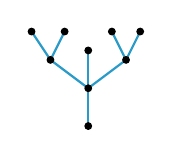
\begin{tikzpicture}[dot/.style={circle, fill=black, inner sep=0pt, minimum size=3pt},
        connector/.style={cyan!80!black, thick},
        baseline=-0.5ex, scale=0.6]
        % Tree: Root connected to a Hub. Hub splits into 3 branches.
        % Left/Right branches split again. Middle branch is a leaf.
        \coordinate (root) at (0,-0.8);
        \coordinate (hub) at (0,0);
        
        \coordinate (l) at (-0.8, 0.6);
        \coordinate (m) at (0, 0.8);
        \coordinate (r) at (0.8, 0.6);
        
        \coordinate (l1) at (-1.2, 1.2);
        \coordinate (l2) at (-0.5, 1.2);
        
        \coordinate (r1) at (0.5, 1.2);
        \coordinate (r2) at (1.1, 1.2);
        
        % Edges
        \draw[cyan!80!black, thick] (root)--(hub);
        \draw[cyan!80!black, thick] (hub)--(l);
        \draw[cyan!80!black, thick] (hub)--(m);
        \draw[cyan!80!black, thick] (hub)--(r);
        
        \draw[cyan!80!black, thick] (l)--(l1);
        \draw[cyan!80!black, thick] (l)--(l2);
        
        \draw[cyan!80!black, thick] (r)--(r1);
        \draw[cyan!80!black, thick] (r)--(r2);
        
        % Nodes
        \foreach \p in {root, hub, l, m, r, l1, l2, r1, r2} \filldraw (\p) circle (2pt);
    \end{tikzpicture}
    \textbf{\color{green!60!black}is a tree}.

    \item[2)]

    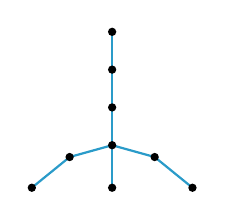
\begin{tikzpicture}[
        % Define styles for consistency
        dot/.style={circle, fill=black, inner sep=0pt, minimum size=3pt},
        connector/.style={cyan!80!black, thick},
        baseline=-0.5ex, scale=0.6
    ]

        % --- Coordinates ---
        % Central Hub
        \coordinate (hub) at (0,0);
        
        % Vertical Spine (going up)
        \coordinate (top1) at (0, 0.8);
        \coordinate (top2) at (0, 1.6);
        \coordinate (top3) at (0, 2.4);
        
        % Bottom Leg
        \coordinate (bot) at (0, -0.9);
        
        % Left Branch
        \coordinate (left_mid) at (-0.9, -0.25);
        \coordinate (left_end) at (-1.7, -0.9);
        
        % Right Branch
        \coordinate (right_mid) at (0.9, -0.25);
        \coordinate (right_end) at (1.7, -0.9);

        % --- Draw Edges (drawn first so they appear behind nodes) ---
        % Spine connections
        \draw[connector] (top3) -- (top2);
        \draw[connector] (top2) -- (top1);
        \draw[connector] (top1) -- (hub);
        
        % Bottom connection
        \draw[connector] (hub) -- (bot);
        
        % Left branch connections
        \draw[connector] (hub) -- (left_mid);
        \draw[connector] (left_mid) -- (left_end);
        
        % Right branch connections
        \draw[connector] (hub) -- (right_mid);
        \draw[connector] (right_mid) -- (right_end);

        % --- Draw Nodes ---
        \node[dot] at (hub) {};
        \node[dot] at (top1) {};
        \node[dot] at (top2) {};
        \node[dot] at (top3) {};
        \node[dot] at (bot) {};
        \node[dot] at (left_mid) {};
        \node[dot] at (left_end) {};
        \node[dot] at (right_mid) {};
        \node[dot] at (right_end) {};

    \end{tikzpicture}
    \textbf{\color{green!60!black}is a tree}.

    \item[3)]
    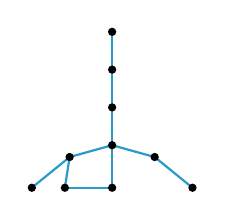
\begin{tikzpicture}[
        % Define styles for consistency
        dot/.style={circle, fill=black, inner sep=0pt, minimum size=3pt},
        connector/.style={cyan!80!black, thick},
        baseline=-0.5ex, scale=0.6
    ]

        % --- Coordinates ---
        % Central Hub
        \coordinate (hub) at (0,0);
        
        % Vertical Spine (going up)
        \coordinate (top1) at (0, 0.8);
        \coordinate (top2) at (0, 1.6);
        \coordinate (top3) at (0, 2.4);
        
        % Bottom Leg
        \coordinate (bot) at (0, -0.9);
        
        % Left Branch
        \coordinate (left_mid) at (-0.9, -0.25);
        \coordinate (left_end) at (-1.7, -0.9);
        
        % Right Branch
        \coordinate (right_mid) at (0.9, -0.25);
        \coordinate (right_end) at (1.7, -0.9);
        \coordinate (extra) at (-1, -0.9);

        % --- Draw Edges (drawn first so they appear behind nodes) ---
        % Spine connections
        \draw[connector] (top3) -- (top2);
        \draw[connector] (top2) -- (top1);
        \draw[connector] (top1) -- (hub);
        
        % Bottom connection
        \draw[connector] (hub) -- (bot);
        
        % Left branch connections
        \draw[connector] (hub) -- (left_mid);
        \draw[connector] (left_mid) -- (left_end);
        
        % Right branch connections
        \draw[connector] (hub) -- (right_mid);
        \draw[connector] (right_mid) -- (right_end);

        % Cycle connections
        \draw[connector] (left_mid) -- (extra);
        \draw[connector] (bot) -- (extra);

        % --- Draw Nodes ---
        \node[dot] at (hub) {};
        \node[dot] at (top1) {};
        \node[dot] at (top2) {};
        \node[dot] at (top3) {};
        \node[dot] at (bot) {};
        \node[dot] at (left_mid) {};
        \node[dot] at (left_end) {};
        \node[dot] at (right_mid) {};
        \node[dot] at (right_end) {};
        \node[dot] at (extra) {};

    \end{tikzpicture}
    \textbf{\color{red}is not a tree}.

    \item[4)]
    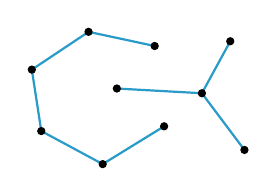
\begin{tikzpicture}[
        % Define styles
        dot/.style={circle, fill=black, inner sep=0pt, minimum size=3pt},
        connector/.style={cyan!80!black, thick},
        baseline=-0.5ex, scale=0.6
    ]

        % --- Coordinates ---
        
        % Left "C" Component
        \coordinate (left_back) at (-2.2, 0.5);
        
        % Top arch
        \coordinate (top_mid) at (-1.0, 1.3);
        \coordinate (top_tip) at (0.4, 1.0);
        
        % Bottom arch
        \coordinate (bot_mid) at (-2.0, -0.8);
        \coordinate (bot_low) at (-0.7, -1.5);
        \coordinate (bot_tip) at (0.6, -0.7);
        
        % Right "Y" Component
        \coordinate (center_tail) at (-0.4, 0.1);
        \coordinate (center_hub) at (1.4, 0.0);
        \coordinate (right_top) at (2.0, 1.1);
        \coordinate (right_bot) at (2.3, -1.2);

        % --- Draw Edges ---
        % Left component connections
        \draw[connector] (left_back) -- (top_mid);
        \draw[connector] (top_mid) -- (top_tip);
        \draw[connector] (left_back) -- (bot_mid);
        \draw[connector] (bot_mid) -- (bot_low);
        \draw[connector] (bot_low) -- (bot_tip);
        
        % Right component connections
        \draw[connector] (center_tail) -- (center_hub);
        \draw[connector] (center_hub) -- (right_top);
        \draw[connector] (center_hub) -- (right_bot);

        % --- Draw Nodes ---
        \node[dot] at (left_back) {};
        \node[dot] at (top_mid) {};
        \node[dot] at (top_tip) {};
        \node[dot] at (bot_mid) {};
        \node[dot] at (bot_low) {};
        \node[dot] at (bot_tip) {};
        \node[dot] at (center_tail) {};
        \node[dot] at (center_hub) {};
        \node[dot] at (right_top) {};
        \node[dot] at (right_bot) {};

    \end{tikzpicture}
    \textbf{\color{red}is not a tree}, but it \textbf{\color{green!60!black}is a forest}.
\end{enumerate}
\end{example}

% 3.4 Lemma
\begin{lemma}
Any tree of order at least 2 has at least two leaves.
\end{lemma}

\begin{proof}
Let $T$ be a tree with $|T| \ge 2$. In particular, $T$ is connected.
Consider a path of maximal length $P=(v_0, v_1, \dots, v_n)$ in $T$. As $|T| \ge 2$, we know that $v_0 \ne v_n$. We claim that $v_0$ and $v_n$ are leaves, i.e. $\deg(v_0)=\deg(v_n)=1$. We execute the argument for $v_0$.
As usual, we know that $N(v_0) \subseteq \{v_1, v_2, \dots, v_n\}$. Let $u \in N(v_0)$ arbitrary, i.e. $u=v_i$ for some $i \ge 1$. But then $(v_0, v_1, \dots, v_i, v_0)$ is a closed walk which is a cycle for all $i \ge 2$. As $T$ does not contain cycles, we conclude that $i=1$ and $v_1$ is the only neighbour of $v_0$. Hence $\deg(v_0)=1$ and $v_0$ is a leaf.
The argument for $v_n$ is analogous.
\end{proof}

% 3.5 Definition
\begin{definition}[Tree Pruning]
Let $T$ be a tree of order at least 3. We denote by \textbf{\color{red}$T^-$} the induced subgraph of $T$ obtained by deleting all leaves of $T$.
\end{definition}

% 3.6 Example
\begin{example}
\begin{enumerate}
    \item[1)] If $T=P_7$ the path of length 6, then $T^- = P_7^- = P_5$ is the path of length 4:
    \begin{center}
    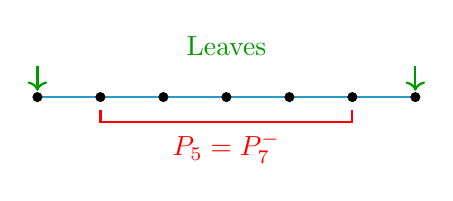
\begin{tikzpicture}[scale=0.8]
        \draw[cyan!80!black, thick] (0,0)--(6,0);
        \foreach \i in {0,...,6} \filldraw (\i,0) circle (2pt);
        
        % Bracket for T^-
        \draw[thick, red] (1,-0.2) -- (1,-0.4) -- (5,-0.4) -- (5,-0.2);
        \node[red, below] at (3,-0.4) {$P_5 = P_7^-$};
        
        % Arrows for leaves
        \draw[->, green!60!black, thick] (0, 0.5) -- (0, 0.1);
        \draw[->, green!60!black, thick] (6, 0.5) -- (6, 0.1);
        \node[green!60!black, above] at (3, 0.5) {Leaves};
    \end{tikzpicture}
    \end{center}

    \item[2)] If $T=K_{1,n}$ the complete bipartite graph, then $T^-=K_1=E_1$ consists of one vertex only:
    \begin{center}
    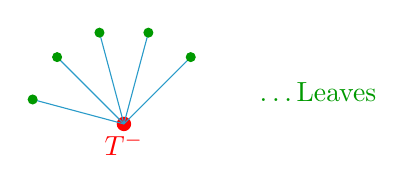
\begin{tikzpicture}[scale=0.8]
        \coordinate (c) at (0,0);
        \filldraw[red] (c) circle (3pt) node[below, red] {$T^-$};
        
        \foreach \i in {1,...,5} {
            \coordinate (l\i) at ({15+\i*30}:1.5);
            \draw[cyan!80!black] (c)--(l\i);
            \filldraw[green!60!black] (l\i) circle (2pt);
        }
        \node[green!60!black, right] at (2, 0.5) {\dots Leaves};
    \end{tikzpicture}
    \end{center}
\end{enumerate}
\end{example}

% 3.7 Lemma
\begin{lemma}
Any tree of order $n$ has exactly $n-1$ edges.
\end{lemma}

\begin{proof}
We proceed by induction on $|T|$.
If $|T|=1$, then $T=K_1$, which has zero edges and the claim holds.
Now assume we know that any tree of order $n$ has exactly $n-1$ many edges and consider $T$ of order $n+1$ arbitrary.
By Lemma 3.4, $T$ has a leaf $u$. Clearly, $T-u$ is still connected and of order $n$, whence $T-u$ has exactly $n-1$ edges.
As $u$ was a leaf in $T$, $T$ has exactly one edge more than $T-u$, whence
\[ \|T\| = n = (n+1)-1, \text{ as desired.} \qedhere \]
\end{proof}

% 3.8 Corollary
\begin{corollary}
A forest of order $n$, consisting of $k$-many connected components, has exactly $n-k$ many edges.
\end{corollary}

We will now see that given a graph $G$ is connected, Lemma 3.7 is not only a necessary, but even a sufficient condition for $G$ to be a tree.

% 3.9 Theorem
\begin{theorem}
A graph $G$ of order $n$ is a tree iff it is connected and has exactly $n-1$ many edges.
\end{theorem}

\begin{proof}
``$\Rightarrow$'' Clear by definition of a tree and Lemma 3.7.

``$\Leftarrow$'' Assume $G$ is connected of order $n$ and contains exactly $n-1$ many edges. If $G$ contains a cycle, take any edge $e_1$ within the cycle and consider $G-e_1$. Then $G-e_1$ is still connected and of order $n$. If $G-e_1$ still contains a cycle, we proceed likewise and after $k \le n-1$ many steps we obtain a graph $G-\{e_1, e_2, \dots, e_k\}$ which is of order $n$, connected and without cycles, whence it is a tree. But $G-\{e_1, \dots, e_k\}$ has $(n-1)-k < n-1$ many edges, contradicting Lemma 3.7.
\end{proof}

% 3.10 Theorem
\begin{theorem}
A graph of order $n$ is a tree iff it is acyclic and has $n-1$ many edges.
\end{theorem}

\begin{proof}
``$\Rightarrow$'' Clear.

``$\Leftarrow$'' Assume $G$ is of order $n$ with $n-1$ many edges and acyclic, i.e. $G$ is a forest. But by Corollary 3.8, if $G$ has $k$-many connected components then $\|G\| = n-k = n-1$, whence $k=1$ and $G$ is connected and hence a tree.
\end{proof}

% 3.11 Corollary (Summary)
\begin{corollary}[Summary]
Let $G$ be a graph of order $n$. Then TFAE:
\begin{enumerate}
    \item[1)] $G$ is connected and acyclic (i.e. a tree).
    \item[2)] $G$ is connected and has $n-1$ many edges.
    \item[3)] $G$ is acyclic and has $n-1$ many edges.
\end{enumerate}
\end{corollary}

% 3.12 Homework
\topic{Homework}
Every edge in a tree is a bridge.

% 3.13 Lemma
\begin{lemma}
For any two vertices $u,v \in V_T$ in a tree $T$, there is a unique $uv$-path.
\end{lemma}

\begin{proof}
As $T$ is connected, there clearly is a $uv$-path for any $u,v \in V_T$.
Now assume that $P_1 = (u=x_0, x_1, \dots, x_k=v)$ and $P_2 = (u=y_0, y_1, \dots, y_\ell=v)$ are two distinct $uv$-paths. Then $P_1 \cup P_2$ is again a tree.
Let $i$ be minimal s.t. $x_i \ne y_i$. Then $(P_1 \cup P_2) - y_i y_{i-1}$ is still connected, contradicting the fact that every edge in a tree is a bridge.
\end{proof}

% 3.14 Corollary
\begin{corollary}
Let $T$ be a tree and $v \in V_T$. Then $ecc(v)$ is the length of the longest path starting from $v$.
\end{corollary}

% 3.15 Lemma
\begin{lemma}
Let $T$ be a tree of order at least 2. Consider $u,v \in V_T$ s.t. $ecc(v) = d(u,v)$. Then $u$ is a leaf.
\end{lemma}

\begin{proof}
Let $P=(v=x_0, x_1, \dots, x_k=u)$ be the unique $vu$ path. If $u$ were not a leaf, then it had at least one neighbour $w \notin P$. But then $(v=x_0, x_1, \dots, x_k, w)$ would be a path starting in $v$ and longer than $P$, contradicting Corollary 3.14.
\end{proof}

% 3.16 Lemma
\begin{lemma}
Let $T$ be a tree of order at least 3. Then $C(T) = C(T^-)$.
\end{lemma}

\begin{proof}
\begin{enumerate}
    \item[1)] Show that $C(T) \subseteq T^-$, i.e. $C(T)$ contains no leaf.
    To this end, let $u$ be a leaf and $v$ its unique neighbour. As $|T| \ge 3$, $v$ is not a leaf itself and $d(u,w) = d(v,w) + 1$ for any $w \in V_T \setminus \{u\}$, whence $ecc(u) > ecc(v)$ and hence $u \notin C(T)$.
    
    \item[2)] Show that $ecc_{T^-}(v) = ecc_T(v) - 1$ for every non-leaf $v \in V_T$.
    To that end, consider an arbitrary non-leaf $v \in V_T$ and pick $u \in V_T$ s.t. $d(v,u) = ecc(v)$. By 3.15, $u$ is a leaf. Let $P$ be the unique $vu$-path in $T$ and note that $u$ is the only leaf on $P$. Hence only $u$ will be deleted from $P$ in $T^-$. As this holds for all paths in $T$ starting in $v$ of length $ecc(v)$, we obtain that $ecc_{T^-}(v) = ecc_T(v) - 1$, as desired.
    
    \item[3)] We conclude from 1) + 2) that for any vertex $v \in T^-$,
    $ecc_{T^-}(v) = ecc_T(v) - 1$, whence $v \in C(T)$ iff $v \in C(T^-)$ (and $rad(T^-) = rad(T)-1$).
\end{enumerate}
\end{proof}

% 3.17 Lemma
\begin{lemma}
Let $T$ be a tree. Then $C(T)$ is either $K_1$ or $K_2$.
\end{lemma}

\begin{proof}
We do induction on $|T|$. If $|T|=1$, then $T=K_1$ is its own center and we are done. Similarly for $|T|=2$, where $T=K_2$.
Now assume that the claim holds for all trees of order $n \ge 3$ and consider a tree $T$ with $|T|=n+1$ arbitrary.
By 3.16, we know that $C(T) = C(T^-)$. By 3.4 we know that $T$ contains at least two leaves, whence $|T^-| \le |T|-2 < n$. Hence, by I.H., $C(T) = C(T^-)$ is either $K_2$ or $K_1$ as desired.
\end{proof}

% 3.18 Lemma
\begin{lemma}
Let $T$ be a tree of order $n$ and $G$ an arbitrary graph s.t. $\delta(G) \ge n-1$. Then $G$ contains $T$ as a subgraph.
\end{lemma}

\begin{proof}
We use induction on $|T|$.
If $|T|=1$, then $T=K_1$ is a subgraph of any graph $G$.
Now assume we proved the claim for all trees of order at most $n$. Consider $T$ with $|T|=n+1$ and $G$ with $\delta(G) \ge n$ arbitrary.
Let $u$ be a leaf of $T$ and denote by $T' := T-u$. Then $|T'|=n$, whence $T'$ can be seen as a subgraph of $G$. Let $v$ be the unique neighbour of $u$ in $T$. Then $\deg_G(v) \ge \delta(G) \ge n$, but as $|T'|=n$ and $v$ cannot be its own neighbour, there exist some $u' \in G$ adjacent to $v$ and not contained in $T'$. Hence, the subgraph $(V_{T'} \cup \{u'\}, E_{T'} \cup \{vu'\})$ is the desired subgraph of $G$ isomorphic to $T$.
\end{proof}

\par\vspace{0.5cm}\noindent
\needspace{3\baselineskip}
{\large \underline{\textbf{Summary}}}
\par\vspace{0.2cm}
\begin{enumerate}
    \item[1)] A tree of order $n$ contains exactly $n-1$ edges.
    \item[2)] Any tree of order at least two contains at least two leaves.
    \item[3)] A graph of order $n$ is a tree iff it is connected of size $n-1$.
    \item[4)] A graph of order $n$ is a tree iff it is acyclic and of size $n-1$.
    \item[5)] A graph is a tree iff for any vertices $u,v$ there is a unique $uv$-path.
    \item[6)] The centre of any tree is either $K_1$ or $K_2$.
    \item[7)] Any graph $G$ contains any tree of order at most $\delta(G)+1$ as a subgraph.
\end{enumerate}

\section{Spanning Trees}

% 3.19 Definition
\begin{definition}
Let $G$ be any graph. We call a subgraph $T \subseteq G$ a \textbf{\color{red}spanning tree} for $G$ if it is a tree and contains all vertices of $G$.
\end{definition}

% 3.20 Remark
\begin{remark}
From the previous chapter it is clear that a spanning tree of a graph $G$ of order $n$ has $n$ many vertices and $n-1$ many edges.
\end{remark}

% 3.21 Examples
\begin{example}
Consider the following graphs and spanning trees.
\begin{enumerate}
    \item[1)] $G = C_6$, a possible spanning tree:
    \begin{center}
    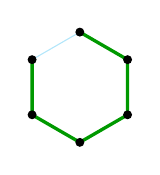
\begin{tikzpicture}[scale=0.7, baseline=(current bounding box.center)]
        % Hexagon
        \foreach \i in {1,...,6} \coordinate (v\i) at (90+60-60*\i : 1);
        
        % Base graph (faint)
        \draw[cyan!30, thin] (v1)--(v2)--(v3)--(v4)--(v5)--(v6)--(v1);
        
        % Spanning Tree (Green Path) - Missing v6-v1 edge
        \draw[green!60!black, very thick] (v1)--(v2)--(v3)--(v4)--(v5)--(v6);
        
        \foreach \i in {1,...,6} \filldraw (v\i) circle (2pt);
    \end{tikzpicture}
    \hspace{0.5cm} $\longrightarrow$ \hspace{0.5cm}
    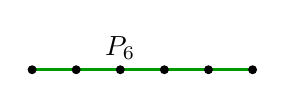
\begin{tikzpicture}[scale=0.7, baseline=(current bounding box.center)]
        % Linear Path P6
        \foreach \i in {1,...,6} \coordinate (u\i) at (\i*0.8, 0);
        \draw[green!60!black, very thick] (u1)--(u2)--(u3)--(u4)--(u5)--(u6);
        \foreach \i in {1,...,6} \filldraw (u\i) circle (2pt);
        \node[above, black] at (u3) {$P_6$};
    \end{tikzpicture}
    \end{center}

    \item[2)] $G = K_5$, possible spanning trees:
    \begin{center}
    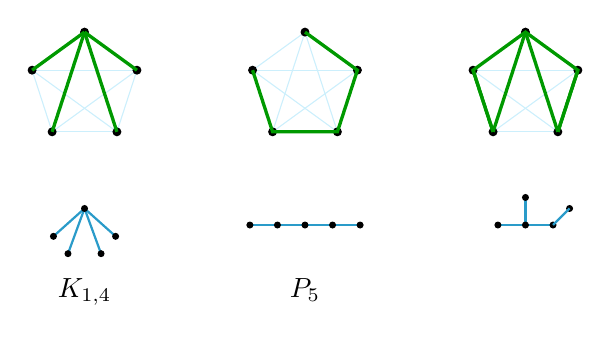
\begin{tikzpicture}[scale=0.7]
        % Define coordinates for pentagons
        \def\pentagon{
            \foreach \i in {1,...,5} \coordinate (v\i) at (90+72-72*\i : 1);
            % Faint complete graph background
            \foreach \i in {1,...,5} \foreach \j in {\i,...,5} 
                \draw[cyan!20, thin] (v\i) -- (v\j);
            \foreach \i in {1,...,5} \filldraw (v\i) circle (2pt);
        }

        % --- Column 1: Star K1,4 ---
        \begin{scope}[xshift=0cm]
            \pentagon
            % Green Edges (Star at top v1)
            \draw[green!60!black, very thick] (v1)--(v2);
            \draw[green!60!black, very thick] (v1)--(v3);
            \draw[green!60!black, very thick] (v1)--(v4);
            \draw[green!60!black, very thick] (v1)--(v5);
            
            % Abstract drawing below
            \begin{scope}[yshift=-2.5cm]
                \coordinate (c) at (0,0.3);
                \foreach \a in {200, 240, 300, 340} 
                    \draw[cyan!80!black, thick] (c) -- (\a:0.6);
                \foreach \a in {200, 240, 300, 340} 
                    \filldraw (\a:0.6) circle (1.5pt);
                \filldraw (c) circle (1.5pt);
                \node[below] at (0,-0.8) {$K_{1,4}$};
            \end{scope}
        \end{scope}

        % --- Column 2: Path P5 ---
        \begin{scope}[xshift=4cm]
            \pentagon
            % Green Edges (Path around perimeter)
            \draw[green!60!black, very thick] (v1)--(v2)--(v3)--(v4)--(v5);
            
            % Abstract drawing below
            \begin{scope}[yshift=-2.5cm]
                \draw[cyan!80!black, thick] (-1,0) -- (1,0);
                \foreach \x in {-1, -0.5, 0, 0.5, 1} \filldraw (\x,0) circle (1.5pt);
                \node[below] at (0,-0.8) {$P_5$};
            \end{scope}
        \end{scope}

        % --- Column 3: Branched Tree (Y-shape) ---
        \begin{scope}[xshift=8cm]
            \pentagon
            % Green Edges (Branched)
            % v1 connected to v2, v5. v2 connected to v3. v5 connected to v4.
            % Path v3-v2-v1-v5-v4
            \draw[green!60!black, very thick] (v3)--(v2)--(v1)--(v5)--(v4);
            % Wait, let's look at the notes "branch" drawing again.
            % It looks like Top connected to BotLeft and BotRight.
            % BotLeft connected to Left. BotRight connected to Right.
            % Let's draw that structure on the pentagon.
            \draw[green!60!black, very thick] (v2)--(v3); % Left to BotLeft
            \draw[green!60!black, very thick] (v3)--(v1); % BotLeft to Top
            \draw[green!60!black, very thick] (v1)--(v4); % Top to BotRight
            \draw[green!60!black, very thick] (v4)--(v5); % BotRight to Right
            
            % Abstract drawing below (T-shape/Y-shape)
            \begin{scope}[yshift=-2.5cm]
                \draw[cyan!80!black, thick] (0,0) -- (0,0.5); % Stem
                \draw[cyan!80!black, thick] (-0.5,0) -- (0.5,0); % Bar
                \filldraw (0,0) circle (1.5pt); \filldraw (0,0.5) circle (1.5pt);
                \filldraw (-0.5,0) circle (1.5pt); \filldraw (0.5,0) circle (1.5pt);
                \filldraw (0.8,0.3) circle (1.5pt); \draw[cyan!80!black, thick] (0.5,0) -- (0.8,0.3); % Extra branch
            \end{scope}
        \end{scope}
    \end{tikzpicture}
    \end{center}
\end{enumerate}
\end{example}

% 3.22 Lemma
\begin{lemma}
Every connected graph contains at least one spanning tree.
\end{lemma}

\begin{proof}
Assume $G$ is connected and let $T$ be a subgraph of $G$ of maximal order s.t. $T$ is a tree. We need to show that $V_T = V_G$.
Otherwise, as $G$ is connected, there is some vertex $u \in V_G \setminus V_T$ which is adjacent to some vertex $v \in V_T$. Now, consider the new subgraph $\hat{T} = (V_T \cup \{u\}, E_T \cup \{uv\})$. As $\deg_{\hat{T}}(u)=1$, $u$ is not contained in any cycles in $\hat{T}$, whence $\hat{T}$ is still a tree. As this contradicts maximality of $|T|$, we conclude that $T$ must contain all vertices of $G$, whence it is a spanning tree for $G$.
\end{proof}

% 3.24 Definition

\begin{definition}
A function $w: E_G \to \mathbb{R}$ is called a \textbf{\color{red}weight function} on $G$.
A graph $G$ together with a weight function (i.e. the triple $(V_G, E_G, w)$) is called a \textbf{\color{red}weighted graph}.
\end{definition}

% 3.25 Example - Visualisation
\begin{example}[Visualisation]
    

We visualise the weighting of a graph by denoting the weight $w(e)$ on top of the edge $e$, e.g.

\begin{center}
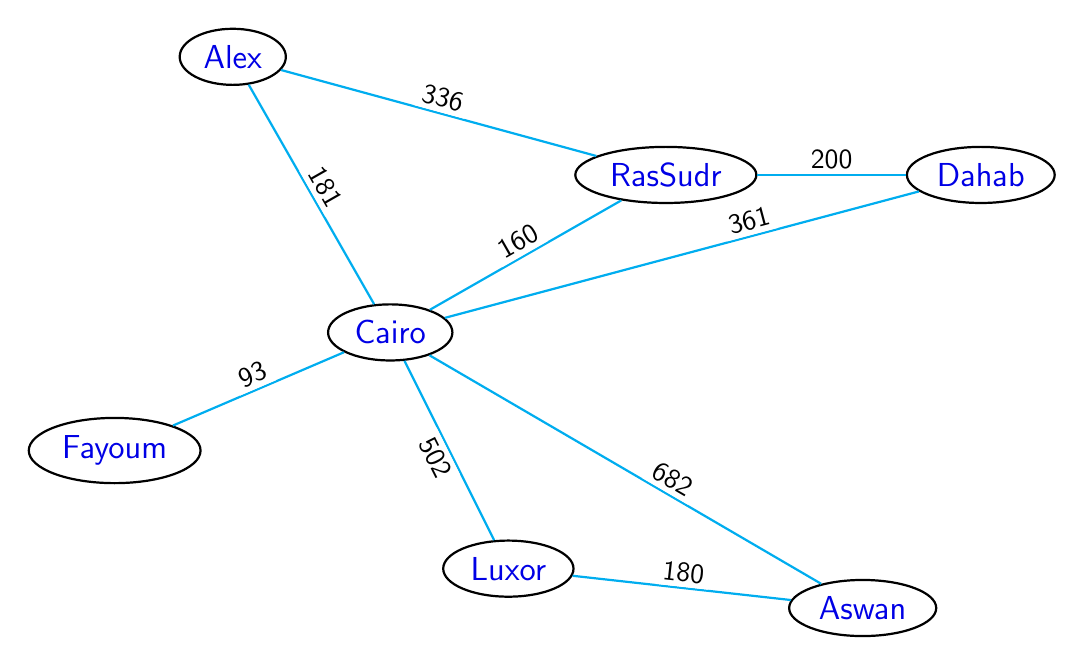
\begin{tikzpicture}[
    % Define specific styles to match the drawing
    city/.style={
        ellipse,
        draw=black,
        thick,
        text=blue!90!black, % Blue text
        font=\sffamily\large,
        inner sep=3pt,
        align=center
    },
    route/.style={
        draw=cyan,
        thick
    },
    label_dist/.style={
        fill=white,    % White background covers the line behind the text
        text=black,
        font=\sffamily,
        sloped,        % Rotates the text to follow the line
        inner sep=2pt
    }
]

    % --- Coordinates / Nodes ---
    % Central Hub
    \node[city] (cairo) at (0,0) {Cairo};
    
    % North / West
    \node[city] (alex) at (-2, 3.5) {Alex};
    \node[city] (fayoum) at (-3.5, -1.5) {Fayoum};
    
    % East / Sinai
    \node[city] (rassudr) at (3.5, 2.0) {RasSudr};
    \node[city] (dahab) at (7.5, 2.0) {Dahab};
    
    % South
    \node[city] (luxor) at (1.5, -3.0) {Luxor};
    \node[city] (aswan) at (6.0, -3.5) {Aswan};

    % --- Edges and Distance Labels ---
    
    % Alex Connections
    \draw[route] (alex) -- (cairo) node[label_dist, midway, above] {181};
    \draw[route] (alex) -- (rassudr) node[label_dist, midway, above] {336};
    
    % Cairo Connections
    \draw[route] (cairo) -- (fayoum) node[label_dist, midway, above] {93};
    \draw[route] (cairo) -- (rassudr) node[label_dist, midway, above] {160};
    \draw[route] (cairo) -- (dahab) node[label_dist, pos=0.65, above] {361};
    \draw[route] (cairo) -- (luxor) node[label_dist, midway, below] {502};
    \draw[route] (cairo) -- (aswan) node[label_dist, pos=0.6, above] {682};
    
    % Other Connections
    \draw[route] (rassudr) -- (dahab) node[label_dist, midway, above] {200};
    \draw[route] (luxor) -- (aswan) node[label_dist, midway, above] {180};

\end{tikzpicture}
\end{center}
Here the weight function of an edge $e=uv$ is given by the (birds eye) distance between $u$ and $v$.
\end{example}

% 3.26 Example
\begin{example}
Consider the following weighted graph.
\begin{center}
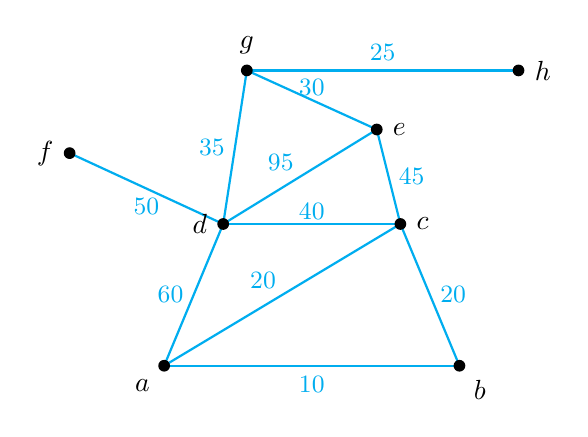
\begin{tikzpicture}[
    scale=1.5,
    node_style/.style={circle, fill=black, inner sep=1.5pt},
    edge_style/.style={cyan, thick},
    weight_style/.style={cyan, font=\small}
]
    % Coordinates
    \coordinate (a) at (0,0);
    \coordinate (b) at (2.5,0);
    \coordinate (c) at (2,1.2);
    \coordinate (d) at (0.5,1.2);
    \coordinate (e) at (1.8,2);
    \coordinate (g) at (0.7,2.5);
    \coordinate (f) at (-0.8,1.8);
    \coordinate (h) at (3.0,2.5);

    % Edges with weights
    \draw[edge_style] (a) -- (b) node[midway, below, weight_style] {10};
    \draw[edge_style] (a) -- (d) node[midway, left, weight_style] {60};
    \draw[edge_style] (a) -- (c) node[midway, above left=-2pt, weight_style] {20};
    \draw[edge_style] (b) -- (c) node[midway, right, weight_style] {20};
    \draw[edge_style] (c) -- (d) node[midway, above=-2pt, weight_style] {40};
    \draw[edge_style] (c) -- (e) node[midway, right, weight_style] {45};
    \draw[edge_style] (d) -- (e) node[midway, above left=-2pt, weight_style] {95};
    \draw[edge_style] (d) -- (g) node[midway, left, weight_style] {35};
    \draw[edge_style] (d) -- (f) node[midway, below, weight_style] {50};
    \draw[edge_style] (g) -- (e) node[midway, above=-2pt, weight_style] {30};
    \draw[edge_style] (g) -- (h) node[midway, above, weight_style] {25};

    % Nodes and Labels
    \node[node_style, label=below left:$a$] at (a) {};
    \node[node_style, label=below right:$b$] at (b) {};
    \node[node_style, label=right:$c$] at (c) {};
    \node[node_style, label=left:$d$] at (d) {};
    \node[node_style, label=right:$e$] at (e) {};
    \node[node_style, label=above:$g$] at (g) {};
    \node[node_style, label=left:$f$] at (f) {};
    \node[node_style, label=right:$h$] at (h) {};
\end{tikzpicture}
\end{center}

We can find several spanning trees. Let's name some and compute their weight.

\vspace{0.5cm}

\begin{minipage}[t]{0.45\textwidth}
    \begin{center}
    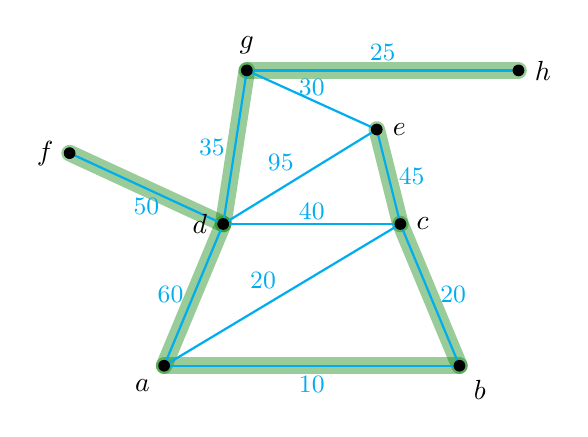
\begin{tikzpicture}[
        scale=1.5,
        node_style/.style={circle, fill=black, inner sep=1.5pt},
        edge_style/.style={cyan, thick},
        weight_style/.style={cyan, font=\small},
        highlight/.style={draw=green!50!black, opacity=0.4, line width=6pt, line cap=round}
    ]
        % Coordinates
        \coordinate (a) at (0,0);
        \coordinate (b) at (2.5,0);
        \coordinate (c) at (2,1.2);
        \coordinate (d) at (0.5,1.2);
        \coordinate (e) at (1.8,2);
        \coordinate (g) at (0.7,2.5);
        \coordinate (f) at (-0.8,1.8);
        \coordinate (h) at (3.0,2.5);

        % Green Highlights (Spanning Tree)
        % Edges: f-d, d-a, a-b, a-c, c-e, d-g, g-h
        \draw[highlight] (f) -- (d);
        \draw[highlight] (d) -- (a);
        \draw[highlight] (a) -- (b);
        \draw[highlight] (b) -- (c);
        \draw[highlight] (c) -- (e);
        \draw[highlight] (d) -- (g);
        \draw[highlight] (g) -- (h);

        % Standard Edges
        \draw[edge_style] (a) -- (b) node[midway, below, weight_style] {10};
        \draw[edge_style] (a) -- (d) node[midway, left, weight_style] {60};
        \draw[edge_style] (a) -- (c) node[midway, above left=-2pt, weight_style] {20};
        \draw[edge_style] (b) -- (c) node[midway, right, weight_style] {20};
        \draw[edge_style] (c) -- (d) node[midway, above=-2pt, weight_style] {40};
        \draw[edge_style] (c) -- (e) node[midway, right, weight_style] {45};
        \draw[edge_style] (d) -- (e) node[midway, above left=-2pt, weight_style] {95};
        \draw[edge_style] (d) -- (g) node[midway, left, weight_style] {35};
        \draw[edge_style] (d) -- (f) node[midway, below, weight_style] {50};
        \draw[edge_style] (g) -- (e) node[midway, above=-2pt, weight_style] {30};
        \draw[edge_style] (g) -- (h) node[midway, above, weight_style] {25};

        % Nodes
        \node[node_style, label=below left:$a$] at (a) {};
        \node[node_style, label=below right:$b$] at (b) {};
        \node[node_style, label=right:$c$] at (c) {};
        \node[node_style, label=left:$d$] at (d) {};
        \node[node_style, label=right:$e$] at (e) {};
        \node[node_style, label=above:$g$] at (g) {};
        \node[node_style, label=left:$f$] at (f) {};
        \node[node_style, label=right:$h$] at (h) {};
    \end{tikzpicture}
    \end{center}
    \textbf{Total weight:} \\
    $45+20+10+60+50+35+25$ \\
    $= 245$
\end{minipage}
\hfill
\begin{minipage}[t]{0.45\textwidth}
    \begin{center}
    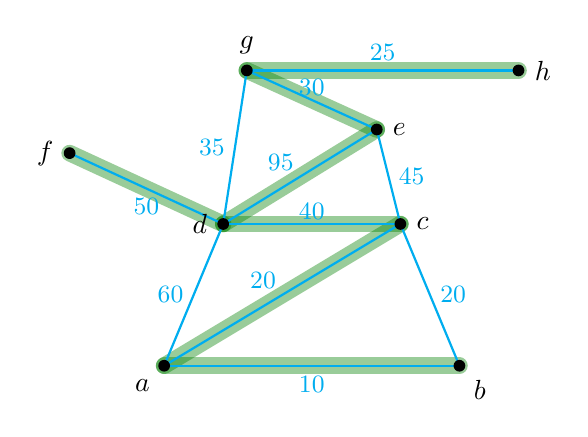
\begin{tikzpicture}[
        scale=1.5,
        node_style/.style={circle, fill=black, inner sep=1.5pt},
        edge_style/.style={cyan, thick},
        weight_style/.style={cyan, font=\small},
        highlight/.style={draw=green!50!black, opacity=0.4, line width=6pt, line cap=round}
    ]
        % Coordinates
        \coordinate (a) at (0,0);
        \coordinate (b) at (2.5,0);
        \coordinate (c) at (2,1.2);
        \coordinate (d) at (0.5,1.2);
        \coordinate (e) at (1.8,2);
        \coordinate (g) at (0.7,2.5);
        \coordinate (f) at (-0.8,1.8);
        \coordinate (h) at (3.0,2.5);

        % Green Highlights (Spanning Tree)
        % Edges: f-d, d-e, e-g, g-h, d-c, c-b, b-a
        \draw[highlight] (f) -- (d);
        \draw[highlight] (d) -- (e);
        \draw[highlight] (e) -- (g);
        \draw[highlight] (g) -- (h);
        \draw[highlight] (d) -- (c);
        \draw[highlight] (c) -- (a);
        \draw[highlight] (b) -- (a);

        % Standard Edges
        \draw[edge_style] (a) -- (b) node[midway, below, weight_style] {10};
        \draw[edge_style] (a) -- (d) node[midway, left, weight_style] {60};
        \draw[edge_style] (a) -- (c) node[midway, above left=-2pt, weight_style] {20};
        \draw[edge_style] (b) -- (c) node[midway, right, weight_style] {20};
        \draw[edge_style] (c) -- (d) node[midway, above=-2pt, weight_style] {40};
        \draw[edge_style] (c) -- (e) node[midway, right, weight_style] {45};
        \draw[edge_style] (d) -- (e) node[midway, above left=-2pt, weight_style] {95};
        \draw[edge_style] (d) -- (g) node[midway, left, weight_style] {35};
        \draw[edge_style] (d) -- (f) node[midway, below, weight_style] {50};
        \draw[edge_style] (g) -- (e) node[midway, above=-2pt, weight_style] {30};
        \draw[edge_style] (g) -- (h) node[midway, above, weight_style] {25};

        % Nodes
        \node[node_style, label=below left:$a$] at (a) {};
        \node[node_style, label=below right:$b$] at (b) {};
        \node[node_style, label=right:$c$] at (c) {};
        \node[node_style, label=left:$d$] at (d) {};
        \node[node_style, label=right:$e$] at (e) {};
        \node[node_style, label=above:$g$] at (g) {};
        \node[node_style, label=left:$f$] at (f) {};
        \node[node_style, label=right:$h$] at (h) {};
    \end{tikzpicture}
    \end{center}
    \textbf{Total weight:} \\
    $10+20+40+50+95+30+25$ \\
    $= 270$
\end{minipage}
\end{example}

% 3.27 Definition
\begin{definition}
Let $(G,w)$ be a connected weighted tree. A \textbf{\color{red}minimum-weight spanning tree} $T$ is a spanning tree of $G$ s.t. the sum of the weights of its edges is minimal among all possible spanning trees of $G$, i.e. if $\tilde{T}$ is another spanning tree, then $\sum_{e \in E_T} w(e) \le \sum_{e \in E_{\tilde{T}}} w(e)$.
\end{definition}

Now how can we find a minimal spanning tree effectively?
Consider the following algorithm:

% 3.28 Kruskal's Algorithm
\topic{Kruskal's Algorithm (1956)}
Consider the set of vertices as a forest $F=(V_G, \emptyset)$ where each vertex is a maximal subtree of $F$. Let $E := E_G$.

\textbf{While} ($F$ is not a tree $\land \ E \ne \emptyset$)
\begin{itemize}
    \item Pick $e \in E$ of minimal weight. Let $E := E \setminus \{e\}$.
    \item If $e$ connects two trees in $F$, let $E_F = E_F \cup \{e\}$.
    \item (i.e. $F+e$ is still acyclic)
\end{itemize}
This algorithm stops after at most $|E_G|$ many repetitions.

% 3.29 Example
\begin{example}
We apply the algorithm on the following weighted graph:

\begin{center}
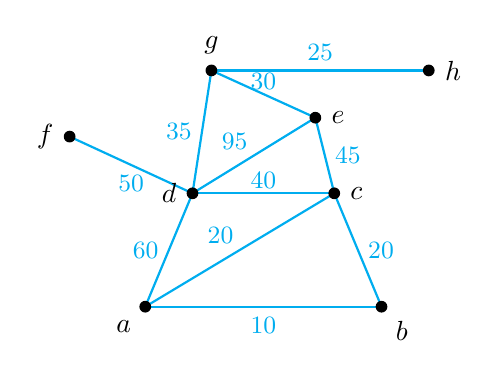
\begin{tikzpicture}[
    scale=1.2,
    node_style/.style={circle, fill=black, inner sep=1.5pt},
    edge_style/.style={cyan, thick},
    weight_style/.style={cyan, font=\small}
]
    % Coordinates
    \coordinate (a) at (0,0);
    \coordinate (b) at (2.5,0);
    \coordinate (c) at (2,1.2);
    \coordinate (d) at (0.5,1.2);
    \coordinate (e) at (1.8,2);
    \coordinate (g) at (0.7,2.5);
    \coordinate (f) at (-0.8,1.8);
    \coordinate (h) at (3.0,2.5);

    % Edges with weights
    \draw[edge_style] (a) -- (b) node[midway, below, weight_style] {10};
    \draw[edge_style] (a) -- (d) node[midway, left, weight_style] {60};
    \draw[edge_style] (a) -- (c) node[midway, above left=-2pt, weight_style] {20};
    \draw[edge_style] (b) -- (c) node[midway, right, weight_style] {20};
    \draw[edge_style] (c) -- (d) node[midway, above=-2pt, weight_style] {40};
    \draw[edge_style] (c) -- (e) node[midway, right, weight_style] {45};
    \draw[edge_style] (d) -- (e) node[midway, above left=-2pt, weight_style] {95};
    \draw[edge_style] (d) -- (g) node[midway, left, weight_style] {35};
    \draw[edge_style] (d) -- (f) node[midway, below, weight_style] {50};
    \draw[edge_style] (g) -- (e) node[midway, above=-2pt, weight_style] {30};
    \draw[edge_style] (g) -- (h) node[midway, above, weight_style] {25};

    % Nodes and Labels
    \node[node_style, label=below left:$a$] at (a) {};
    \node[node_style, label=below right:$b$] at (b) {};
    \node[node_style, label=right:$c$] at (c) {};
    \node[node_style, label=left:$d$] at (d) {};
    \node[node_style, label=right:$e$] at (e) {};
    \node[node_style, label=above:$g$] at (g) {};
    \node[node_style, label=left:$f$] at (f) {};
    \node[node_style, label=right:$h$] at (h) {};
\end{tikzpicture}
\end{center}

Let us mark edges we add to $F$ green and the ones we disregard, red.

\vspace{1em}

% --- The Algorithm Steps (Wrapped in a minipage to keep them together) ---
\noindent
\begin{minipage}{\textwidth}
    % Common TikZ settings for the small graphs
    \tikzset{
        tiny_graph/.style={
            scale=0.85, % INCREASED SCALE FOR 2 COLUMNS
            baseline=(current bounding box.center),
            node_style/.style={circle, fill=black, inner sep=1.5pt},
            edge_style/.style={cyan, thick},
            weight_style/.style={cyan, font=\tiny}, 
            highlight/.style={draw=green!50!black, opacity=0.4, line width=4pt, line cap=round},
            highlightred/.style={draw=red!100!black, opacity=1, line width=4pt, line cap=round}
        }
    }

    % --- ROW 1 (Steps 1 & 2) ---
    \begin{minipage}[t]{0.48\textwidth}
        \textbf{1)} $E=E_G, E_F=\emptyset$ \\
        \begin{tikzpicture}[tiny_graph]
            \coordinate (a) at (0,0); \coordinate (b) at (2.5,0); \coordinate (c) at (2,1.2);
            \coordinate (d) at (0.5,1.2); \coordinate (e) at (1.8,2); \coordinate (g) at (0.7,2.5);
            \coordinate (f) at (-0.8,1.8); \coordinate (h) at (3.0,2.5);
            \draw[edge_style] (a)--(b) (a)--(d) (a)--(c) (b)--(c) (c)--(d) (c)--(e) (d)--(e) (d)--(g) (d)--(f) (g)--(e) (g)--(h);
            \foreach \p in {a,b,c,d,e,g,f,h} \node[node_style] at (\p) {};
        \end{tikzpicture}
    \end{minipage}%
    \hfill
    \begin{minipage}[t]{0.48\textwidth}
        \textbf{2)} $E=E-\{ab\}, E_F=\{ab\}$ \\
        \begin{tikzpicture}[tiny_graph]
            \coordinate (a) at (0,0); \coordinate (b) at (2.5,0); \coordinate (c) at (2,1.2);
            \coordinate (d) at (0.5,1.2); \coordinate (e) at (1.8,2); \coordinate (g) at (0.7,2.5);
            \coordinate (f) at (-0.8,1.8); \coordinate (h) at (3.0,2.5);
            \draw[highlight] (a)--(b);
            \draw[edge_style] (a)--(b) (a)--(d) (a)--(c) (b)--(c) (c)--(d) (c)--(e) (d)--(e) (d)--(g) (d)--(f) (g)--(e) (g)--(h);
            \foreach \p in {a,b,c,d,e,g,f,h} \node[node_style] at (\p) {};
        \end{tikzpicture}
    \end{minipage}
    
    \vspace{1.5em}

    % --- ROW 2 (Steps 3 & 4) ---
    \begin{minipage}[t]{0.48\textwidth}
        \textbf{3)} $E=E-\{ac\}, E_F=E_F \cup \{ac\}$ \\
        \begin{tikzpicture}[tiny_graph]
            \coordinate (a) at (0,0); \coordinate (b) at (2.5,0); \coordinate (c) at (2,1.2);
            \coordinate (d) at (0.5,1.2); \coordinate (e) at (1.8,2); \coordinate (g) at (0.7,2.5);
            \coordinate (f) at (-0.8,1.8); \coordinate (h) at (3.0,2.5);
            \draw[highlight] (a)--(b) (a)--(c);
            \draw[edge_style] (a)--(b) (a)--(d) (a)--(c) (b)--(c) (c)--(d) (c)--(e) (d)--(e) (d)--(g) (d)--(f) (g)--(e) (g)--(h);
            \foreach \p in {a,b,c,d,e,g,f,h} \node[node_style] at (\p) {};
        \end{tikzpicture}
    \end{minipage}%
    \hfill
    \begin{minipage}[t]{0.48\textwidth}
        \textbf{4)} $E=E-\{bc\}, E_F=E_F$ \\
        \begin{tikzpicture}[tiny_graph]
            \coordinate (a) at (0,0); \coordinate (b) at (2.5,0); \coordinate (c) at (2,1.2);
            \coordinate (d) at (0.5,1.2); \coordinate (e) at (1.8,2); \coordinate (g) at (0.7,2.5);
            \coordinate (f) at (-0.8,1.8); \coordinate (h) at (3.0,2.5);
            \draw[highlight] (a)--(b) (a)--(c);
            \draw[highlightred] (b)--(c);
            \draw[edge_style] (a)--(b) (a)--(d) (a)--(c) (b)--(c) (c)--(d) (c)--(e) (d)--(e) (d)--(g) (d)--(f) (g)--(e) (g)--(h);
            \foreach \p in {a,b,c,d,e,g,f,h} \node[node_style] at (\p) {};
        \end{tikzpicture}
    \end{minipage}

    \vspace{1.5em}

    % --- ROW 3 (Steps 5 & 6) ---
    \begin{minipage}[t]{0.48\textwidth}
        \textbf{5)} $E=E-\{gh\}, E_F=E_F \cup \{gh\}$ \\
        \begin{tikzpicture}[tiny_graph]
            \coordinate (a) at (0,0); \coordinate (b) at (2.5,0); \coordinate (c) at (2,1.2);
            \coordinate (d) at (0.5,1.2); \coordinate (e) at (1.8,2); \coordinate (g) at (0.7,2.5);
            \coordinate (f) at (-0.8,1.8); \coordinate (h) at (3.0,2.5);
            \draw[highlight] (a)--(b) (a)--(c) (g)--(h);
            \draw[highlightred] (b)--(c);
            \draw[edge_style] (a)--(b) (a)--(d) (a)--(c) (b)--(c) (c)--(d) (c)--(e) (d)--(e) (d)--(g) (d)--(f) (g)--(e) (g)--(h);
            \foreach \p in {a,b,c,d,e,g,f,h} \node[node_style] at (\p) {};
        \end{tikzpicture}
    \end{minipage}%
    \hfill
    \begin{minipage}[t]{0.48\textwidth}
        \textbf{6)} $E=E-\{ge\}, E_F=E_F \cup \{ge\}$ \\
        \begin{tikzpicture}[tiny_graph]
            \coordinate (a) at (0,0); \coordinate (b) at (2.5,0); \coordinate (c) at (2,1.2);
            \coordinate (d) at (0.5,1.2); \coordinate (e) at (1.8,2); \coordinate (g) at (0.7,2.5);
            \coordinate (f) at (-0.8,1.8); \coordinate (h) at (3.0,2.5);
            \draw[highlight] (a)--(b) (a)--(c) (g)--(h) (g)--(e);
            \draw[highlightred] (b)--(c);
            \draw[edge_style] (a)--(b) (a)--(d) (a)--(c) (b)--(c) (c)--(d) (c)--(e) (d)--(e) (d)--(g) (d)--(f) (g)--(e) (g)--(h);
            \foreach \p in {a,b,c,d,e,g,f,h} \node[node_style] at (\p) {};
        \end{tikzpicture}
    \end{minipage}

    \vspace{1.5em}

    % --- ROW 4 (Steps 7 & 8) ---
    \begin{minipage}[t]{0.48\textwidth}
        \textbf{7)} $E=E-\{gd\}, E_F=E_F \cup \{gd\}$ \\
        \begin{tikzpicture}[tiny_graph]
            \coordinate (a) at (0,0); \coordinate (b) at (2.5,0); \coordinate (c) at (2,1.2);
            \coordinate (d) at (0.5,1.2); \coordinate (e) at (1.8,2); \coordinate (g) at (0.7,2.5);
            \coordinate (f) at (-0.8,1.8); \coordinate (h) at (3.0,2.5);
            \draw[highlight] (a)--(b) (a)--(c) (g)--(h) (g)--(e) (g)--(d);
            \draw[highlightred] (b)--(c);
            \draw[edge_style] (a)--(b) (a)--(d) (a)--(c) (b)--(c) (c)--(d) (c)--(e) (d)--(e) (d)--(g) (d)--(f) (g)--(e) (g)--(h);
            \foreach \p in {a,b,c,d,e,g,f,h} \node[node_style] at (\p) {};
        \end{tikzpicture}
    \end{minipage}%
    \hfill
    \begin{minipage}[t]{0.48\textwidth}
        \textbf{8)} $E=E-\{cd\}, E_F=E_F \cup \{cd\}$ \\
        \begin{tikzpicture}[tiny_graph]
            \coordinate (a) at (0,0); \coordinate (b) at (2.5,0); \coordinate (c) at (2,1.2);
            \coordinate (d) at (0.5,1.2); \coordinate (e) at (1.8,2); \coordinate (g) at (0.7,2.5);
            \coordinate (f) at (-0.8,1.8); \coordinate (h) at (3.0,2.5);
            \draw[highlight] (a)--(b) (a)--(c) (g)--(h) (g)--(e) (g)--(d) (c)--(d);
            \draw[highlightred] (b)--(c);
            \draw[edge_style] (a)--(b) (a)--(d) (a)--(c) (b)--(c) (c)--(d) (c)--(e) (d)--(e) (d)--(g) (d)--(f) (g)--(e) (g)--(h);
            \foreach \p in {a,b,c,d,e,g,f,h} \node[node_style] at (\p) {};
        \end{tikzpicture}
    \end{minipage}

    \vspace{1.5em}

    % --- ROW 5 (Steps 9 & 10) ---
    \begin{minipage}[t]{0.48\textwidth}
        \textbf{9)} $E=E-\{ce\}, E_F=E_F$ \\
        \begin{tikzpicture}[tiny_graph]
            \coordinate (a) at (0,0); \coordinate (b) at (2.5,0); \coordinate (c) at (2,1.2);
            \coordinate (d) at (0.5,1.2); \coordinate (e) at (1.8,2); \coordinate (g) at (0.7,2.5);
            \coordinate (f) at (-0.8,1.8); \coordinate (h) at (3.0,2.5);
            \draw[highlight] (a)--(b) (a)--(c) (g)--(h) (g)--(e) (g)--(d) (c)--(d);
            \draw[highlightred] (b)--(c) (e)--(c);
            \draw[edge_style] (a)--(b) (a)--(d) (a)--(c) (b)--(c) (c)--(d) (c)--(e) (d)--(e) (d)--(g) (d)--(f) (g)--(e) (g)--(h);
            \foreach \p in {a,b,c,d,e,g,f,h} \node[node_style] at (\p) {};
        \end{tikzpicture}
    \end{minipage}%
    \hfill
    \begin{minipage}[t]{0.48\textwidth}
        \textbf{10)} $E=E-\{df\}, E_F=E_F \cup \{df\}$ \\
        \begin{tikzpicture}[tiny_graph]
            \coordinate (a) at (0,0); \coordinate (b) at (2.5,0); \coordinate (c) at (2,1.2);
            \coordinate (d) at (0.5,1.2); \coordinate (e) at (1.8,2); \coordinate (g) at (0.7,2.5);
            \coordinate (f) at (-0.8,1.8); \coordinate (h) at (3.0,2.5);
            \draw[highlight] (a)--(b) (a)--(c) (g)--(h) (g)--(e) (g)--(d) (c)--(d) (f)--(d);
            \draw[highlightred] (b)--(c) (e)--(c);
            \draw[edge_style] (a)--(b) (a)--(d) (a)--(c) (b)--(c) (c)--(d) (c)--(e) (d)--(e) (d)--(g) (d)--(f) (g)--(e) (g)--(h);
            \foreach \p in {a,b,c,d,e,g,f,h} \node[node_style] at (\p) {};
        \end{tikzpicture}
    \end{minipage}
    
\end{minipage}

\vspace{1em}

Here the algorithm stops, as 
$F = (V_G, E_F)$ with $E_F = \{ab, ac, gh, eg, dg, cd, df\}$ 
is a single tree whence the conditions in 
the while loop are violated.\\
(The output is the spanning tree $F$. Note that the second condition 
in the while loop was still valid, as $E = \{ad, de\} \neq \emptyset$).
\end{example}

% 3.30 Theorem
\begin{theorem}
Kruskal's algorithm is correct, i.e. it always terminates and its output is a minimum-weight spanning tree.
\end{theorem}

\begin{proof}
\begin{enumerate}
    \item[1)] Termination: As after $|E_G|$-many steps the condition $E \ne \emptyset$ is violated, the algorithm always terminates.
    \item[2)] The output $F$ is a spanning tree:
    As $V_F=V_G$, it clearly contains all vertices of $G$.
    Further, in each step the regarded edge $e$ either connects two disconnected trees into one larger tree, or, if it would connect two vertices of the same subtree in $F$, is disregarded. Hence after each step, $F$ is still a forest, i.e. acyclic.
    It remains to show that $F$ is connected. If the algorithm stops because $F$ is a tree, then it is clearly connected. If it stops because we went through all the edges, then any edge of $G$ not contained in $F$ would connect two vertices of the same connected component. Thus $F$ has as many connected components as $G$, which is one, as $G$ is connected.
    \item[3)] $F$ is a minimum-weight spanning tree.
    Aiming for a contradiction, assume this is not the case. Let $\{e_1, \dots, e_{n-1}\}$ be all the edges in $F$, enumerated in the order they were added to $F$ by the algorithm.
    Among all possible minimum-weight spanning trees, let $T$ be one that agrees with $F$ on the largest initial segment of $(e_1, \dots, e_{n-1})$, i.e. if $k$ is the smallest index s.t. $e_{k+1} \notin T$, then there is no minimum-weight spanning tree which contains $\{e_1, \dots, e_{k+1}\}$.
    As by assumption $F$ is not minimum-weight, we have $k < n-1$.
    As $T$ is a spanning tree which does not contain $e_{k+1}$, we know that $T+e_{k+1}$ contains a cycle $C$. As $F$ did not contain cycles, there is one edge $e \in C \subseteq T$ which is not in $F$.
    Now $T+e_{k+1}-e$ is a connected graph of order $n$ and size $n-1$, whence still a spanning tree. It contains the edges $\{e_1, \dots, e_k, e_{k+1}\}$, hence it can no longer be of minimum weight. This means that $w(e_{k+1}) > w(e)$.
    But as $e \notin F$ and in particular $e \notin \{e_1, \dots, e_k\}$ this means $e$ was available at the step of the algorithm after we added $e_k$ and of less weight than $e_{k+1}$. This contradicts the assumption that the algorithm chooses the edge of minimal weight which keeps $F$ acyclic. \qedhere
\end{enumerate}
\end{proof}

% 3.31 Lemma
\begin{lemma}
If $G$ is a connected weighted graph s.t. distinct edges have distinct weights, then there is a unique minimum-weight spanning tree.
\end{lemma}

\begin{proof}
Homework.
\end{proof}
% \chapter{Euler and Hamilton}

\section{Euler}
% Imagine (Unnumbered Header)
\par\vspace{0.5cm}\noindent
\needspace{3\baselineskip}
{\large \underline{\textbf{Imagine}}}
\par\vspace{0.2cm}
A salesperson with their wagon wants to pass by every street in his neighbourhood to sell their goods. Of course, they want to minimize efforts, so they would like to avoid passing the same street twice. These type of problems are considered when discussing \textbf{\color{red}Eulerian graphs}.

Then, as only few people buy, they switch to their car and only visit a central place in each city of the area. Again, to improve efficiency, they only want to visit each city once. This type of problem is studied when discussing \textbf{\color{red}Hamiltonian graphs}.

How do these two problems differ? Let's find out!

% 4.1 Definition
\begin{definition}
We call a trail in a graph $G$ an \textbf{\color{red}Eulerian trail} if it contains every edge of $G$. We call it an \textbf{\color{red}Eulerian circuit} if it is a closed Eulerian trail. Finally, the graph $G$ itself is called an \textbf{\color{red}Eulerian graph} iff it contains an Eulerian circuit.
\end{definition}

% 4.2 Examples
\begin{example}
\begin{enumerate}
    \item[1)]
    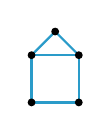
\begin{tikzpicture}[scale=0.6, baseline=(current bounding box.center)]
        \coordinate (a) at (0,0); \coordinate (b) at (1,0);
        \coordinate (c) at (1,1); \coordinate (d) at (0,1);
        \coordinate (e) at (0.5,1.5);
        \draw[cyan!80!black, thick] (a)--(b)--(c)--(d)--(a);
        \draw[cyan!80!black, thick] (d)--(e)--(c);
        \foreach \p in {a,b,c,d,e} \filldraw (\p) circle (2pt);
    \end{tikzpicture}
    \textbf{\color{blue}is not} Eulerian, but has an Eulerian trail.

    \item[2)]
    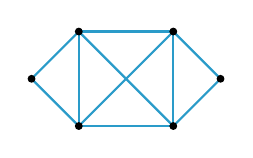
\begin{tikzpicture}[scale=0.6, baseline=(current bounding box.center)]
        % Left node, Central Box, Right node
        \coordinate (l) at (-2,0);
        \coordinate (tl) at (-1,1);
        \coordinate (bl) at (-1,-1);
        \coordinate (tr) at (1,1);
        \coordinate (br) at (1,-1);
        \coordinate (r) at (2,0);

        % Wings
        \draw[cyan!80!black, thick] (l)--(tl);
        \draw[cyan!80!black, thick] (l)--(bl);
        \draw[cyan!80!black, thick] (r)--(tr);
        \draw[cyan!80!black, thick] (r)--(br);

        % Central K4
        \draw[cyan!80!black, thick] (tl)--(tr)--(br)--(bl)--(tl); % Outer Box
        \draw[cyan!80!black, thick] (tl)--(br); % Diagonal
        \draw[cyan!80!black, thick] (bl)--(tr); % Diagonal

        \foreach \p in {l,tl,bl,tr,br,r} \filldraw (\p) circle (2pt);
    \end{tikzpicture}
    \textbf{\color{green!60!black}is indeed} Eulerian.

    \item[3)] Any cycle $C_n$ is clearly Eulerian.
    
    \item[4)] Any path of length $n \ge 1$ is \textbf{\color{red}not} Eulerian but has an Eulerian trail.

    \item[5)]
    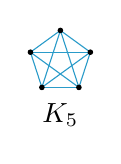
\begin{tikzpicture}[scale=0.4, baseline=(current bounding box.center)]
        \foreach \i in {1,...,5} \coordinate (v\i) at (90+72*\i:1);
        \foreach \i in {1,...,5} \foreach \j in {\i,...,5} \draw[cyan!80!black] (v\i)--(v\j);
        \foreach \i in {1,...,5} \filldraw (v\i) circle (2pt);
        \node[below] at (0,-1) {$K_5$};
    \end{tikzpicture}
    \textbf{\color{green!60!black}is indeed} Eulerian, but

    \item[6)]
    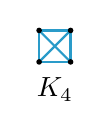
\begin{tikzpicture}[scale=0.4, baseline=(current bounding box.center)]
        \coordinate (a) at (0,0); \coordinate (b) at (1,0);
        \coordinate (c) at (1,1); \coordinate (d) at (0,1);
        \draw[cyan!80!black, thick] (a)--(b)--(c)--(d)--(a);
        \draw[cyan!80!black, thick] (a)--(c); \draw[cyan!80!black, thick] (b)--(d);
        \foreach \p in {a,b,c,d} \filldraw (\p) circle (2pt);
        \node[below] at (0.5,-0.2) {$K_4$};
    \end{tikzpicture}
    \textbf{\color{red}does not even contain} an Eulerian trail.

    \item[7)] Generally, every $K_{2n+1}$ is Eulerian and every $K_{2n+2}$ does not even contain an Eulerian trail for $n \ge 1$.
\end{enumerate}
\end{example}

% 4.3 Observation
\topic{Observation}

Consider the graph $K_5$. We observe the following properties:
\begin{enumerate}
    \item[1)] $K_5$ is Eulerian: $(a,b,c,d,e,a,d,b,e,c,a)$ is an Eulerian circuit.
    \begin{center}
    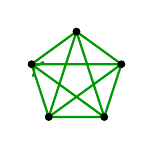
\begin{tikzpicture}[scale=0.6]
        \foreach \i in {1,...,5} \coordinate (v\i) at (90+72*\i:1);
        \foreach \i in {1,...,5} \foreach \j in {\i,...,5} \draw[cyan!20, thin] (v\i)--(v\j);
        \draw[green!60!black, thick, ->] (v1)--(v2)--(v3)--(v4)--(v5)--(v1)--(v4)--(v2)--(v5)--(v3)--(v1);
        \foreach \i in {1,...,5} \filldraw (v\i) circle (2pt);
    \end{tikzpicture}
    \end{center}

    \item[2)] Every vertex of $K_5$ has an even degree. (All 4).
    \begin{center}
    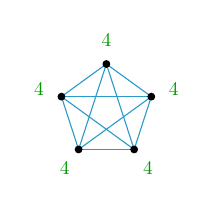
\begin{tikzpicture}[scale=0.6]
        \foreach \i in {1,...,5} \coordinate (v\i) at (90+72*\i:1);
        \foreach \i in {1,...,5} \foreach \j in {\i,...,5} \draw[cyan!80!black] (v\i)--(v\j);
        \foreach \i in {1,...,5} \filldraw (v\i) circle (2pt) node[anchor=center, shift={(90+72*\i:0.3)}, scale=0.7, green!60!black] {4};
    \end{tikzpicture}
    \end{center}
    
    \item[3)] We can partition $E_{K_5}$ into cycles (i.e. find mutually edge-disjoint cycles that together use all edges of $K_5$).
    
    \vspace{0.3cm}
    
    \begin{minipage}[t]{0.45\textwidth}
        \centering
        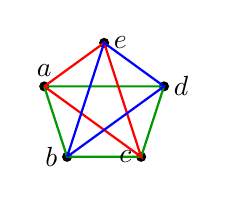
\begin{tikzpicture}[scale=0.8]
            \foreach \i in {1,...,5} \coordinate (v\i) at (90+72*\i:1);
            \foreach \i in {1,...,5} \filldraw (v\i) circle (2pt);
            
            % Decomposition 1: C1(green), C2(red), C3(blue)
            \draw[green!60!black, thick] (v1)--(v2)--(v3)--(v4)--(v1); % 4-cycle
            \draw[red, thick] (v1)--(v3)--(v5)--(v1); % Triangle
            \draw[blue, thick] (v2)--(v4)--(v5)--(v2); % Triangle
            
            \node[above] at (v1) {$a$}; \node[left] at (v2) {$b$}; \node[left] at (v3) {$c$};
            \node[right] at (v4) {$d$}; \node[right] at (v5) {$e$};
        \end{tikzpicture}
        \\
        {\color{green!60!black}$C_1=(a,b,c,d)$} \\
        {\color{red}$C_2=(a,c,e)$} \\
        {\color{blue}$C_3=(b,d,e)$}
    \end{minipage}
    \textbf{or}
    \begin{minipage}[t]{0.45\textwidth}
        \centering
        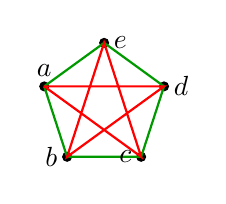
\begin{tikzpicture}[scale=0.8]
            \foreach \i in {1,...,5} \coordinate (v\i) at (90+72*\i:1);
            \foreach \i in {1,...,5} \filldraw (v\i) circle (2pt);
            
            % Decomposition 2: Two 5-cycles
            \draw[green!60!black, thick] (v1)--(v2)--(v3)--(v4)--(v5)--(v1); % Outer
            \draw[red, thick] (v1)--(v3)--(v5)--(v2)--(v4)--(v1); % Inner star
            
            \node[above] at (v1) {$a$}; \node[left] at (v2) {$b$}; \node[left] at (v3) {$c$};
            \node[right] at (v4) {$d$}; \node[right] at (v5) {$e$};
        \end{tikzpicture}
        \\
        {\color{green!60!black}$C_1=(a,b,c,d,e,a)$} \\
        {\color{red}$C_2=(a,c,e,b,d,a)$}
    \end{minipage}
\end{enumerate}

These three properties do not appear together by coincidence. It turns out, they are equivalent to each other.

% 4.4 Auxiliary Lemma
\begin{lemma}[Auxiliary Lemma]
Let $G$ be a connected graph with $|G| \ge 2$. If $\deg(v)$ is even for all $v \in V_G$, then $G$ contains a cycle $C$. Moreover, $G-C$ still contains a cycle or is $E_{|G|}$.
\end{lemma}

\begin{proof}
Assume $G$ is as above. If $G$ would not contain a cycle, it was a tree. But then it had to contain a leaf $v$. But then $\deg(v)=1$ is not even \textbf{\color{red}$\lightning$}.
For the ``moreover'' part, observe that
\[ \deg^{G-C}(v) = \begin{cases} \deg^G(v)-2 & \text{if } v \in V_C \\ \deg^G(v) & \text{else} \end{cases} \]
hence still even. Then each connected component of $G-C$ still contains a cycle (whence so does $G-C$), or is of order 1.
\end{proof}

% 4.5 Theorem
\begin{theorem}[Euler-Hierholzer-Veblen]
Let $G$ be a connected graph. The following are equivalent:
\begin{enumerate}
    \item[1)] $G$ is Eulerian.
    \item[2)] Every vertex of $G$ is of even degree.
    \item[3)] The edge set of $G$ can be partitioned into a set of edge-disjoint cycles.
\end{enumerate}
\end{theorem}

% 4.6 Corollary
\begin{corollary}
A graph contains an Eulerian trail iff either each vertex has even degree or there are exactly two vertices of odd degree.
\end{corollary}

\begin{proof}
Proof of Theorem 4.5:
As all three clearly hold for $|G|=1$, we may assume that $|G|>1$.

\underline{$1) \Rightarrow 2)$}: Assume $G$ is Eulerian. Let $Q$ be an Eulerian circuit of $G$. Now consider $v \in V_G$ arbitrary. Without loss of generalisation, we may assume that $Q$ does not start with $v$. Now, every appearence of $v$ in $Q$ corresponds to two distinct edges involving $v$, the one leading \textit{into} $v$ and the one leading \textit{away} from $v$. As $Q$ is Eulerian, it uses all edges incident with $v$ whence in total there is an even number of edges incident with $v$ and $\deg(v)$ is even. \checkmark

\underline{$2) \Rightarrow 3)$}: Assume $G$ only contains vertices of even degree. By Lemma 4.4, $G$ contains at least one cycle $C$. We proceed by induction on the number $n$ of cycles in $C$.
\textbf{n=1}: If $G$ contains only one cycle, then $G=C_{|G|}$ and hence the desired partition of edges is just the cycle $G$ itself.
\textbf{n $\to$ n+1}: Now assume every graph containing at most $n$-many cycles allows a partition into edge-disjoint cycles. Consider any connected $G$ with $(n+1)$-many cycles. Pick an arbitrary cycle $C$ in $G$. Then as in 4.4, in $H := (V_G, E_G - E_C)$, every vertex still has even degree. Now, every connected component of $H$ contains at most $n$-many cycles. By induction hypothesis, we can partition each connected component of $H$, and hence $H$ itself, into edge-disjoint cycles. Once we add $C$ to this partition, we obtain the desired partition of $G$. \checkmark (Note that this gives you a cooking recipe of how to find cycles).

\underline{$3) \Rightarrow 1)$}: Assume the edge set of $G$ can be partitioned into $k$-many sets $S_1, S_2, \dots, S_k$ s.t. the edges of each $S_i$ form a cycle.
Let $Q$ be a circuit of maximal length in $G$ s.t. the edges of $Q$ equals the union of some sets $S_i$, i.e. such that there is $I \subseteq \{1, \dots, k\}$ with $E_Q = \bigcup_{i \in I} S_i$.
As the $S_i$ are pairwise disjoint, we know that $Q$ contains either no edge from $S_i$ or all edges from $S_i$ for every $i \le k$.
Now, if $E_Q = E_G$, then $G$ is Eulerian and we are done.
Otherwise, there is some edge not contained in $Q$, but incident with a vertex $v$ in $Q$. The edge must be contained in exactly one $S_\ell$ with $\ell \notin I$. Note that $Q$ and $S_\ell$ have no common edges, but they share the vertex $v$. Hence we may glue the circuit $Q$ and the cycle $S_\ell$ at $v$ and obtain a new circuit $Q'$ longer than $Q$ with $E_{Q'} = \bigcup_{i \in I \cup \{\ell\}} S_i$, contradicting our choice of $Q$.
Hence $Q$ contained all edges of $G$ and hence $G$ is Eulerian. \checkmark
\end{proof}

\section{Hamilton}

\textbf{Sir William Rowan Hamilton (1805--1865)}
\begin{itemize}
    \item Irish pure mathematician
    \item Contributions to optics, mechanics and algebra.
    \item Also invented a game (The Icosian Game) build on graph theory (bought by Jaques and Son, huge failure).
\end{itemize}

% 4.7 Definition
\begin{definition}
Let $G$ be a graph. A \textbf{\color{red}Hamiltonian path} is a path in $G$ which uses all vertices of $G$. A \textbf{\color{red}Hamiltonian cycle} is a cycle in $G$ which uses all of $V_G$.
We call $G$ \textbf{\color{red}traceable} if it contains a Hamiltonian path and we call it \textbf{\color{red}Hamiltonian} if it contains a Hamiltonian cycle.
\end{definition}

% 4.8 Remark
\begin{remark}
\begin{enumerate}
    \item[1)] Every Hamiltonian graph is traceable but not vice versa.
    \item[2)] Traceable graphs are connected.
    \item[3)] If $|G|=n$, then $G$ is Hamiltonian iff it contains $C_n$ as a subgraph and it is traceable iff it contains $P_n$ as a subgraph.
\end{enumerate}
\end{remark}

% 4.9 Examples
\begin{example}
\begin{enumerate}
    % Item 1: C6
    \item 
    \begin{minipage}[t]{0.6\textwidth}
        $C_6$ \textbf{\color{green!60!black}is Hamiltonian} via $v_1 \dots v_6 v_1$. \\
        {\color{blue!80!black}\small All vertices have even degree.}
    \end{minipage}
    \begin{minipage}[t]{0.3\textwidth}
        \centering
        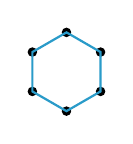
\begin{tikzpicture}[scale=0.5, baseline=(current bounding box.north)]
            \foreach \i in {1,...,6} \filldraw (90+60-60*\i:1) circle (3pt);
            \draw[cyan!80!black, thick] (90:1) -- (30:1) -- (-30:1) -- (-90:1) -- (210:1) -- (150:1) -- cycle;
        \end{tikzpicture}
    \end{minipage}

    % Item 2: K4
    \item 
    \begin{minipage}[t]{0.6\textwidth}
        $K_4$ \textbf{\color{green!60!black}is Hamiltonian} via $v_1 v_2 v_3 v_4 v_1$. \\
        {\color{blue!80!black}\small All vertices have odd degree.}
    \end{minipage}
    \begin{minipage}[t]{0.3\textwidth}
        \centering
        
\begin{tikzpicture}[scale=0.5, baseline=(current bounding box.north)]
            \coordinate (a) at (0,1); \coordinate (b) at (1,0);
            \coordinate (c) at (0,-1); \coordinate (d) at (-1,0);
            \draw[cyan!80!black, thick] (a)--(b)--(c)--(d)--(a);
            \draw[cyan!80!black, thick] (a)--(c); \draw[cyan!80!black, thick] (b)--(d);
            \foreach \p in {a,b,c,d} \filldraw (\p) circle (3pt);
        \end{tikzpicture}
    \end{minipage}

    % Item 3: G1 (Wheel graph)
    \item 
    \begin{minipage}[t]{0.6\textwidth}
        The graph $G_1$ \textbf{\color{green!60!black}is Hamiltonian}. \\
        {\color{blue!80!black}\small There are vertices of even and odd degree.}
    \end{minipage}
    \begin{minipage}[t]{0.3\textwidth}
        \centering
        
\begin{tikzpicture}[scale=0.4, baseline=(current bounding box.north)]
            \coordinate (c) at (0,0);
            \foreach \i in {1,...,8} \coordinate (v\i) at (90+45-45*\i:1.2);
            \draw[cyan!80!black, thick] (v1)--(v2)--(v3)--(v4)--(v5)--(v6)--(v7)--(v8)--(v1);
            \foreach \i in {1,...,8} \draw[cyan!80!black, thick] (c)--(v\i);
            \foreach \i in {1,...,8} \filldraw (v\i) circle (3pt); \filldraw (c) circle (3pt);
        \end{tikzpicture}
    \end{minipage}

    % Item 4: G2 (Two squares sharing a vertex)
    \item 
    \begin{minipage}[t]{0.6\textwidth}
        The graph $G_2$ is \textbf{not} Hamiltonian. \\
        {\color{blue!80!black}\small Every vertex has even degree.}
    \end{minipage}
    \begin{minipage}[t]{0.3\textwidth}
        \centering
        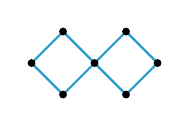
\begin{tikzpicture}[scale=0.4, baseline=(current bounding box.north)]
            % Two diamonds touching
            \coordinate (c) at (0,0);
            \coordinate (t1) at (-1,1); \coordinate (b1) at (-1,-1); \coordinate (l1) at (-2,0);
            \coordinate (t2) at (1,1); \coordinate (b2) at (1,-1); \coordinate (r2) at (2,0);
            
            % Left diamond
            \draw[cyan!80!black, thick] (c)--(t1)--(l1)--(b1)--(c);
            % Right diamond
            \draw[cyan!80!black, thick] (c)--(t2)--(r2)--(b2)--(c);
            
            \foreach \p in {c,t1,b1,l1,t2,b2,r2} \filldraw (\p) circle (3pt);
        \end{tikzpicture}
    \end{minipage}

    % Item 5: K1,3
    \item 
    \begin{minipage}[t]{0.6\textwidth}
        The graph $K_{1,3}$ is \textbf{not} Hamiltonian. \\
        {\color{blue!80!black}\small All vertices have odd degree.}
    \end{minipage}
    \begin{minipage}[t]{0.3\textwidth}
        \centering
        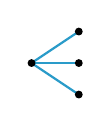
\begin{tikzpicture}[scale=0.4, baseline=(current bounding box.north)]
            \coordinate (c) at (0,0);
            \coordinate (r1) at (1.5, 1); \coordinate (r2) at (1.5, 0); \coordinate (r3) at (1.5, -1);
            \draw[cyan!80!black, thick] (c)--(r1); \draw[cyan!80!black, thick] (c)--(r2); \draw[cyan!80!black, thick] (c)--(r3);
            \foreach \p in {c,r1,r2,r3} \filldraw (\p) circle (3pt);
        \end{tikzpicture}
    \end{minipage}

    % Item 6: P4
    \item 
    \begin{minipage}[t]{0.6\textwidth}
        The path $P_4$ is \textbf{not} Hamiltonian. \\
        {\color{blue!80!black}\small There are vertices of even and odd degree.}
    \end{minipage}
    \begin{minipage}[t]{0.3\textwidth}
        \centering
        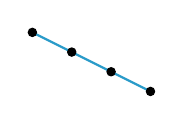
\begin{tikzpicture}[scale=0.5, baseline=(current bounding box.north)]
            \foreach \i in {0,1,2,3} \coordinate (p\i) at (\i, -0.5*\i); % Slanted path
            \draw[cyan!80!black, thick] (p0)--(p1)--(p2)--(p3);
            \foreach \i in {0,1,2,3} \filldraw (p\i) circle (3pt);
        \end{tikzpicture}
    \end{minipage}
\end{enumerate}
\end{example}

% 4.10 Remark
\begin{remark}
While it is rather easy to decide whether a graph is Eulerian (P-TIME, $O(|G|^2)$), it is surprisingly \textbf{hard} to do the same for Hamiltonian graphs. This problem is known to be \textbf{NP-complete} and still we did not manage to find an equivalent condition for Hamiltonianity (other than containing $C_{|G|}$ as a subgraph, which is basically the definition).

We hence see, even though the Eulerian graph problem and the Hamiltonian graph problem seem so similar, their resolution requires very different levels of efforts.
The best we can do at the moment is give some \textbf{sufficient} criteria.
\end{remark}

% 4.11 Theorem
\begin{theorem}[Dirac]
Let $G$ be s.t. $|G| \ge 3$. If $\delta(G) \ge \frac{n}{2}$, then $G$ is Hamiltonian.
\end{theorem}

\begin{proof}
Consider $G$ arbitrary s.t. $|G|=n \ge 3$ and $\delta(G) \ge \frac{n}{2}$.\\
Then $G$ is necessarily connected (think why).\\
Consider a path $P=(v_1, v_2, \dots, v_k)$ of maximal length in $G$.\\
We claim that there is some $j < k$ s.t. $v_{j+1} \in N(v_1)$ and $v_j \in N(v_k)$. i.e.
\begin{center}
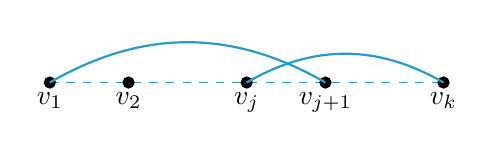
\begin{tikzpicture}[scale=1]
    % Path
    \draw[cyan!80!black, dashed] (0,0) -- (5,0);
    \foreach \x/\l in {0/v_1, 1/v_2, 2.5/v_j, 3.5/v_{j+1}, 5/v_k} \filldraw (\x,0) circle (2pt) node[below] {$\l$};
    % Cross edges
    \draw[cyan!80!black, thick] (0,0) to[bend left] (3.5,0);
    \draw[cyan!80!black, thick] (2.5,0) to[bend left] (5,0);
\end{tikzpicture}
\end{center}
is a subgraph of $P$. Note that as usual, as $P$ is of maximal length, all neighbours of $v_1$ and $v_k$ must be on $P$. As $\delta(G) \ge \frac{n}{2}$, $v_k$ has at least $\frac{n}{2}$ many neighbours $v_j$ in $P$. Aiming for a contradiction, assume for every neighbour $v_j \in N(v_k)$, $v_{j+1} \notin N(v_1)$. Then there are at least $\frac{n}{2}$ many vertices in $P$ which are \textbf{not} neighbours of $v_1$. This now yields the desired contradiction, as all neighbours of $v_1$ are on $P$ and thus $\deg(v_1) \le (k-1) - \frac{n}{2} \le (n-1) - \frac{n}{2} = \frac{n}{2} - 1 < \frac{n}{2}$, contradicting $\delta(G) \ge \frac{n}{2}$.
Hence there is some $j$ s.t. $v_1 v_{j+1}$ and $v_j v_k$ are edges, which leads to the existence of a cycle
\[ C = (v_1, v_2, \dots, v_j, v_k, v_{k-1}, \dots, v_{j+1}, v_1). \]
\begin{center}
\begin{tikzpicture}[scale=0.8]
    % Visualizing the Posa rotation cycle
    \draw[cyan!80!black, thick] (0,0)--(1,0)--(2,0) node[midway, below] {$\dots$}--(3,0)--(4,0)--(5,0);
    \draw[red, thick, ->] (0,0) to[bend left] (4,0);
    \draw[red, thick, ->] (3,0) to[bend right] (5,0);
    \filldraw (0,0) circle (2pt) node[below] {$v_1$};
    \filldraw (5,0) circle (2pt) node[below] {$v_k$};
    \filldraw (3,0) circle (2pt) node[below] {$v_j$};
    \filldraw (4,0) circle (2pt) node[below] {$v_{j+1}$};
\end{tikzpicture}
\end{center}
Finally, we claim that $C$ is indeed a Hamiltonian cycle, i.e. it contains all vertices of $G$. Otherwise, as $G$ is connected, there is a vertex $u$ in $G \setminus C$ which is adjacent to one vertex $v_i$ in $C$. But as $C$ is a cycle, we can form a new path starting in $u, v_i \dots$ and then traveling through all $k-1$ many vertices of $C$. This path is longer than $P$, contradicting our choice of $P$.
Hence, $C$ indeed contains all vertices of $G$ whence it is a Hamiltonian cycle and $G$ is Hamiltonian.
\end{proof}

% 4.12 Fact
\begin{theorem}[{Fact - Ore, 1960}]
Let $G$ be a graph of order $n \ge 3$. Suppose for every pair of non-adjacent vertices $u,v$ we have that $\deg(u) + \deg(v) \ge n$. Then $G$ is Hamiltonian.
\end{theorem}

Note that now Dirac's Theorem is a mere corollary of Ore's theorem.\\
We want to achieve yet another sufficient criterion for Hamiltonicity. This leads us to the so-called independence number.

% 4.13 Definition
\begin{definition}
Let $G$ be a graph. A set $S \subseteq V_G$ of vertices is called an \textbf{\color{red}independent set} if any two vertices in $S$ are nonadjacent.
The \textbf{\color{red}independence number $\alpha(G)$} of $G$ is the maximal size of an independent set.
\end{definition}

% 4.14 Examples
\begin{example}
\begin{itemize}
    \item $\alpha(E_n) = n$, as $V_{E_n}$ is an independent set.
    \item $\alpha(K_n) = 1$, as any two vertices are adjacent. Actually, the converse also holds, i.e. $\alpha(G)=1$ iff $G$ is complete.
    \item $\alpha(K_{n,m}) = \max\{n,m\}$, as any set is independent iff it is contained in one of the parts.
\end{itemize}
\end{example}

% 4.15 Notation
\topic{Notation}
If $P$ is a path and $x,y$ are two vertices on $P$, then we denote by \textbf{\color{red}$P[x,y]$} the subpath on $P$ from $x$ to $y$. E.g. for
\begin{center}
\begin{tikzpicture}[scale=0.8]
    % Path v1 to v7
    \draw[cyan!80!black, thick] (0,0) -- (6,0);
    \foreach \i in {1,...,7} \filldraw (\i-1, 0) circle (2pt) node[below] {$v_\i$};
\end{tikzpicture}
\end{center}
we have $P[v_6, v_3] = (v_6, v_5, v_4, v_3)$.

Similarly, if $C$ is a cycle and $x,y \in C, x \neq y$, then we denote by \textbf{\color{red}$C^+[x,y]$} the $xy$-path on $C$ in clockwise direction and by \textbf{\color{red}$C^-[x,y]$} the $xy$-path on $C$ in counter-clockwise direction.

E.g. if $C$ is
\begin{center}
\begin{tikzpicture}[scale=0.8, baseline=(current bounding box.center)]
    % Octagon C8
    \foreach \i in {1,...,8} \coordinate (v\i) at (90+45-45*\i : 1.2);
    \draw[cyan!80!black, thick] (v1)--(v2)--(v3)--(v4)--(v5)--(v6)--(v7)--(v8)--(v1);
    
    \foreach \i in {1,...,8} \filldraw (v\i) circle (2pt);
    
    % Labels v1..v8
    \node[above] at (v1) {$v_1$}; \node[above right] at (v2) {$v_2$};
    \node[right] at (v3) {$v_3$}; \node[below right] at (v4) {$v_4$};
    \node[below] at (v5) {$v_5$}; \node[below left] at (v6) {$v_6$};
    \node[left] at (v7) {$v_7$}; \node[above left] at (v8) {$v_8$};

    % Red markers x and y (x at v1, y at v4 based on notes)
    \node[red, below=2pt] at (v1) {$x$};
    \node[red, above left=2pt] at (v4) {$y$};
\end{tikzpicture}
\end{center}
then $C^+[x,y] = (v_1, v_2, v_3, v_4)$ and $C^-[x,y] = (v_1, v_8, v_7, v_6, v_5, v_4)$.

Finally, for sequences $s=(x_1, \dots, x_\ell), t=(y_1, \dots, y_k)$ we define \textbf{\color{red}$s \hat{\ } t$} $:= (x_1, \dots, x_\ell, y_1, \dots, y_k)$ to be the concatenation of both.

% 4.16 Theorem
% 4.16 Theorem
\begin{theorem}[{Chv\'atal, Erd\H{o}s, 1972}]
Let $G$ be a graph of order at least 3. If $\kappa(G) \ge \alpha(G)$, then $G$ is Hamiltonian.
\end{theorem}

\begin{proof}
Let $G$ be as above, i.e. $|G| \ge 3, \kappa(G) \ge 1, \kappa(G) \ge \alpha(G)$.
\begin{itemize}
    \item First we argue that $\kappa(G) \ge 2$. Otherwise $\kappa(G)=\alpha(G)=1$, whence $G$ is a complete graph. As further $\kappa(K_n)=n-1$, $G$ would be $K_2$, contradicting $|G| \ge 3$.
    \item Hence now we know that $\kappa(G) \ge 2$. By 1.41(8), we know that $\delta(G) \ge \kappa(G) \ge 2$, whence by 1.39, $G$ contains a cycle.
\end{itemize}

Now consider a cycle $C$ of maximal length in $C$. We claim that $C$ is Hamiltonian.
Aiming for a contradiction, assume $C$ is not Hamiltonian, i.e. there is some vertex $v \notin C$.
Let $H$ be the connected component of $v$ in $G \setminus C$.

\begin{center}
    \includegraphics[width=0.6\textwidth]{./images/pic_4_16_1.png} % Placeholder 1: Setup Diagram (H and C)
\end{center}

Now, we list all elements of $C$ which are connected to some vertex in $H$ in clockwise order: $\{c_1, c_2, \dots, c_r\}$ (s.t. $c_j \in C^+[c_{j-1}, c_{j+1}]$), i.e. where each $c_i$ is adjacent to some $h_i \in H$.

\begin{center}
    \includegraphics[width=0.6\textwidth]{./images/pic_4_16_2.png} % Placeholder 2: c_i definition diagram
\end{center}

\textbf{Claim 1:} No two $c_i$'s are consecutive vertices in $C$.
Proof: Otherwise assume there is an $i$ s.t. $c_{i+1}$ is the clockwise successor of $c_i$. Let $P$ be a path from $h_i$ to $h_{i+1}$ in $H$.
Then $C^+[c_{i+1}, c_i] \hat{\ } (c_i h_i) \hat{\ } P \hat{\ } (h_{i+1} c_{i+1})$ is a cycle strictly longer than $C$, contradicting our assumptions. $\lightning$

\begin{center}
    \includegraphics[width=0.6\textwidth]{./images/pic_4_16_3.png} % Placeholder 3: Claim 1 contradiction diagram
\end{center}

Now that no two $c_i$ and $c_j$ are clockwise successors, we can define the set $D = \{d_1, d_2, \dots, d_r\}$ where each $d_i$ is the clockwise successor of $c_i$ in $C$ and we get that $\{c_1, \dots, c_r\} \cap \{d_1, \dots, d_r\} = \emptyset$.

\begin{center}
    \includegraphics[width=0.6\textwidth]{./images/pic_4_16_4.png} % Placeholder 4: Definition of d_i diagram
\end{center}

\textbf{Claim 2:} $\{c_1, \dots, c_r\}$ is a cut set for $G$.
Proof: This is clear as any path from $v$ to a vertex in $C$ has to pass through one of the vertices in $\{c_1, \dots, c_r\}$, so $G - \{c_1, \dots, c_r\}$ is disconnected.
Consequently, as $\kappa(G)$ is the size of a smallest cut set, we obtain that $r \ge \kappa(G) \ge 2$.

\textbf{Claim 3:} There are $d_i$ and $d_j$ which are adjacent.
Proof: Consider the set $X := \{d_1, d_2, \dots, d_r, v\}$, and recall that there is no edge between any $d_i$ and $v$. As $|X| = r+1 \ge \kappa(G)+1 > \alpha(G)$, $X$ cannot be an independent set, whence at least one pair $d_i, d_j$ must be adjacent.

\begin{center}
    \includegraphics[width=0.6\textwidth]{./images/pic_4_16_5.png} % Placeholder 5: Claim 3 / Edge d_i d_j diagram
\end{center}

Now we are ready for our final contradiction: We produce a cycle $\hat{C}$ longer than $C$. Assume $d_i d_j$ is an edge and $i < j$. Let $q_{h_i h_j}$ be a path in $H$ from $h_i$ to $h_j$.
Now define $\hat{C} = (c_i) \hat{\ } q_{h_i h_j} \hat{\ } (c_j) \hat{\ } C^-[c_j, d_i] \hat{\ } (d_i d_j) \hat{\ } C^+[d_j, c_i]$.

\begin{center}
    \includegraphics[width=0.6\textwidth]{./images/pic_4_16_6.png} % Placeholder 6: Final Cycle Construction diagram
\end{center}

Note that $\hat{C}$ uses all edges of $C$ except the edges $c_i d_i$ and $c_j d_j$. Instead it uses at least the three additional edges $c_i h_i, h_j c_j$ and $d_i d_j$. Hence, $\hat{C}$ is strictly longer than the cycle $C$, which contradicts our choice of $C$.
Conclusively, $C$ must contain all vertices of $G$ and hence is Hamiltonian.
\end{proof}

So far, we have encountered sufficient criteria for Hamiltonian graphs using the degree of vertices and the independence number. We will conclude the chapter by providing a last sufficient criterium using a new concept - \textbf{\color{red}forbidden subgraphs}.

% 4.17 Definition
\begin{definition}
Let $H$ and $G$ be graphs. We say that $G$ is \textbf{\color{red}$H$-free} if $H$ is not (isomorphic to) an induced subgraph of $G$. Moreover, if $S$ is a collection of graphs, then we call $G$ \textbf{\color{red}$S$-free} iff $G$ is $H$-free for any $H \in S$.
\end{definition}

% 4.18 Example
\begin{example}
The Petersen graph
\begin{center}
\begin{tikzpicture}[scale=0.85]
    % --- Left Text Block with Brace ---
    \node[anchor=east] at (-3, 0) {
        $\begin{aligned}
            & \text{is \textbf{\color{green!60!black}indeed} } C_3\text{-free} \\
            & \text{is \textbf{\color{red}not} } C_5\text{-free} \\
            & \text{is \textbf{\color{red}not} } E_4\text{-free} \\
            & \text{is \textbf{\color{green!60!black}indeed} } E_5\text{-free}
        \end{aligned}
        \left\} \parbox{0.5cm}{\vspace{2cm}} \right.$ % Invisible parbox to stretch the brace
    };

    % --- Center: The Graph G ---
    \node at (-2, 0.5) {$G=$};
    \begin{scope}[xshift=0cm]
        % Outer pentagon
        \foreach \i in {1,...,5} \coordinate (o\i) at (90+72*\i:1.5);
        % Inner star
        \foreach \i in {1,...,5} \coordinate (i\i) at (90+72*\i:0.7);
        
        \draw[cyan!80!black, thick] (o1)--(o2)--(o3)--(o4)--(o5)--(o1);
        \draw[cyan!80!black, thick] (i1)--(i3)--(i5)--(i2)--(i4)--(i1);
        \foreach \i in {1,...,5} \draw[cyan!80!black, thick] (o\i)--(i\i);
        \foreach \p in {o1,o2,o3,o4,o5,i1,i2,i3,i4,i5} \filldraw (\p) circle (2pt);
    \end{scope}

    % --- Right: Recall Info ---
    \node[anchor=west, align=left, blue!80!black, scale=0.9] at (2, 0.5) {
        Recall: \\
        $\kappa(G)=3$ \\
        $\alpha(G)=4$
    };

    % --- Bottom Text ---
    \node[anchor=west] at (2, -1) {
        $G$ is hence also $\{C_3, E_5\}$-free.
    };
\end{tikzpicture}
\end{center}
\end{example}

% 4.19 Notations
\topic{Notations}

Let $Z_1$ be the graph $Z_1 =$ 
\begin{tikzpicture}[baseline=-0.5ex, scale=0.4]
    % Triangle with top antenna
    \coordinate (a) at (-0.5,-0.5); \coordinate (b) at (0.5,-0.5); \coordinate (c) at (0,0.5);
    \coordinate (d) at (0,1.2);
    \draw[cyan!80!black, thick] (a)--(b)--(c)--(a);
    \draw[cyan!80!black, thick] (c)--(d);
    \foreach \p in {a,b,c,d} \filldraw (\p) circle (3pt);
\end{tikzpicture}
and $N=$
\begin{tikzpicture}[baseline=-0.5ex, scale=0.4]
    % Triangle with side legs
    \coordinate (a) at (-0.5,0.5); \coordinate (b) at (0.5,0.5); \coordinate (c) at (0,-0.5);
    \coordinate (l) at (-1.2, 0); \coordinate (r) at (1.2, 0);
    % Actually looking at notes N: Triangle base, two legs out
    \draw[cyan!80!black, thick] (a)--(b)--(c)--(a);
    \draw[cyan!80!black, thick] (a)--(-1.2, 0.5);
    \draw[cyan!80!black, thick] (b)--(1.2, 0.5);
    \filldraw (a) circle (3pt); \filldraw (b) circle (3pt); \filldraw (c) circle (3pt);
    \filldraw (-1.2, 0.5) circle (3pt); \filldraw (1.2, 0.5) circle (3pt);
\end{tikzpicture}.

Further, we call the graph $K_{1,3}$ the \textbf{\color{red}claw}, based on its shape:
$K_{1,3} =$ 
\begin{tikzpicture}[baseline=-0.5ex, scale=0.4]
    % Claw shape 1: <
    \coordinate (c) at (0.5,0);
    \draw[cyan!80!black, thick] (c)--(0, 0.5);
    \draw[cyan!80!black, thick] (c)--(-0.2, 0);
    \draw[cyan!80!black, thick] (c)--(0, -0.5);
    \filldraw (c) circle (3pt); \filldraw (0,0.5) circle (3pt); \filldraw (-0.2,0) circle (3pt); \filldraw (0,-0.5) circle (3pt);
\end{tikzpicture}
, or also $K_{1,3} =$ 
\begin{tikzpicture}[baseline=-0.5ex, scale=0.4]
    % Claw shape 2: Y (Mercedes star)
    \coordinate (c) at (0,0.2);
    \draw[cyan!80!black, thick] (c)--(0, 1);
    \draw[cyan!80!black, thick] (c)--(-0.6, -0.5);
    \draw[cyan!80!black, thick] (c)--(0.6, -0.5);
    \filldraw (c) circle (3pt); \filldraw (0,1) circle (3pt); \filldraw (-0.6,-0.5) circle (3pt); \filldraw (0.6,-0.5) circle (3pt);
\end{tikzpicture}.
\\
\\
% 4.20 Theorem
\begin{theorem}[{Goodman, Hedetniemi, 1974}]
Let $G$ be 2-connected and $\{K_{1,3}, Z_1\}$-free, then $G$ is Hamiltonian.
\end{theorem}

\begin{proof}
As $\delta(G) \ge \kappa(G) \ge 2$, we get that $G$ contains a cycle. Consider such a cycle $C$ of maximal length. We claim that $C$ is Hamiltonian.\\
Otherwise, as $G$ is connected, there was a vertex $v \in V_G$ not on $C$ but adjacent to some vertex $x$ on $C$, i.e.
\begin{center}
    \includegraphics[width=0.6\textwidth]{./images/pic_4_20.png} % Placeholder 1: Setup Diagram (H and C)
\end{center}
Denote by $y$ and $z$ the neighbours of $x$ on $C$.\\
Note that $yv$ is not an edge as otherwise replacing the subsequence $(y,x)$ in $C$ by $(y,v,x)$ would yield a cycle longer than $C$. Similarly, $vz$ is not an edge.
Consequently, the induced subgraph on $S=\{x,y,z,v\}$ is either
$\langle S \rangle = K_{1,3}$ 
\begin{tikzpicture}[baseline=-0.5ex, scale=0.4]
    % Claw shape 2: Y (Mercedes star)
    \coordinate (c) at (0,0.2);
    \draw[cyan!80!black, thick] (c)--(0, 1);
    \draw[cyan!80!black, thick] (c)--(-0.6, -0.5);
    \draw[cyan!80!black, thick] (c)--(0.6, -0.5);
    \filldraw (c) circle (3pt); \filldraw (0,1) circle (3pt); \filldraw (-0.6,-0.5) circle (3pt); \filldraw (0.6,-0.5) circle (3pt);
\end{tikzpicture} or $\langle S \rangle = Z_1$, 
\begin{tikzpicture}[baseline=-0.5ex, scale=0.4]
    % Triangle with top antenna
    \coordinate (a) at (-0.5,-0.5); \coordinate (b) at (0.5,-0.5); \coordinate (c) at (0,0.5);
    \coordinate (d) at (0,1.2);
    \draw[cyan!80!black, thick] (a)--(b)--(c)--(a);
    \draw[cyan!80!black, thick] (c)--(d);
    \foreach \p in {a,b,c,d} \filldraw (\p) circle (3pt);
\end{tikzpicture} both of which contradict our assumptions on $G$.
\end{proof}

The following final condition is now easy to verify:

% 4.21 Theorem
\begin{theorem}[{Duffus, Gould, Jacobson, 1980}]
Let $G$ be a $\{K_{1,3}, N\}$-free graph.\\
i) If $G$ is connected, it is traceable.\\
ii) If $G$ is 2-connected, it is Hamiltonian.
\end{theorem}

Note that neither of these are necessary for $G$ to be Hamiltonian. Indeed, for any graph $H$ there is a Hamiltonian graph $G$ which contains $H$ as an induced subgraph.
% \chapter{Planarity}

(lat. planaris -- flat, level)

\begin{definition}
A graph $G$ is called \textbf{\color{red}planar} if it can be drawn on a plane s.t. its edges at most intersect in their end vertices. Any such drawing is then called a \textbf{\color{red}planar representation} or a \textbf{\color{red}planar embedding}. If $G$ is not planar, it is called \textbf{\color{red}nonplanar}.
\end{definition}

\begin{example}
\begin{enumerate}
    \item[1)] Clearly, trees, cycles and empty graphs are planar.
    \item[2)] The graph \begin{tikzpicture}[baseline=(current bounding box.center), scale=0.4]
        \coordinate (a) at (0,0); \coordinate (b) at (1,0); \coordinate (c) at (1,1); \coordinate (d) at (0,1);
        \draw[cyan!80!black, thick] (a)--(b)--(c)--(d)--(a)--(c); \draw[cyan!80!black, thick] (b)--(d);
        \foreach \p in {a,b,c,d} \filldraw (\p) circle (2pt);
    \end{tikzpicture} is planar and this is a planar representation.
    \item[3)] The graph $K_{2,3}$ 
    \begin{tikzpicture}[baseline=(current bounding box.center), scale=0.5]
        \coordinate (a) at (0,0.5); \coordinate (b) at (0,-0.5);
        \coordinate (c) at (1,0.8); \coordinate (d) at (1,0); \coordinate (e) at (1,-0.8);
        \foreach \x in {a,b} \foreach \y in {c,d,e} \draw[cyan!80!black] (\x)--(\y);
        \foreach \p in {a,b,c,d,e} \filldraw (\p) circle (2pt);
        \node[left] at (a) {$a$}; \node[left] at (b) {$b$};
        \node[right] at (c) {$c$}; \node[right] at (d) {$d$}; \node[right] at (e) {$e$};
    \end{tikzpicture}
    is planar, but this is \textbf{not} a planar representation.
    One planar representation is given by
    \begin{tikzpicture}[baseline=(current bounding box.center), scale=0.5]
        % Diamond shape a, d, b, c
        \coordinate (a) at (0,1); \coordinate (d) at (1,0); 
        \coordinate (b) at (0,-1); \coordinate (c) at (-1,0);
        \coordinate (e) at (2,0);
        
        \draw[cyan!80!black, thick] (a)--(c)--(b)--(d)--(a); % Cycle a-c-b-d-a
        \draw[cyan!80!black, thick] (a)--(e)--(b); % Outer connections to e
        
        \filldraw (a) circle (2pt) node[above] {$a$};
        \filldraw (b) circle (2pt) node[below] {$b$};
        \filldraw (c) circle (2pt) node[left] {$c$};
        \filldraw (d) circle (2pt) node[right] {$d$};
        \filldraw (e) circle (2pt) node[right] {$e$};
    \end{tikzpicture}.
\end{enumerate}
\end{example}

In order to prove that a graph is planar, we ``just'' have to provide one planar representation. But these can be very hard to find.
In order to prove that a graph is \underline{not} planar, we would have to check ``all'' possible representations. This is not feasible.
But we can help ourselves by throwing some math on the problem.
To this end, we need some more terminology.

\begin{definition}
A \textbf{\color{red}region} in a planar rep. is a maximal area of the plane s.t. any two points within can be connected by a curve which does not intersect or touch any part of the graph.
Regions which are completely bounded (=surrounded) by graph edges are called \textbf{\color{red}interior regions}. The unique non-interior region is called \textbf{\color{red}exterior region}.
\end{definition}

\begin{example}
Consider the planar representation 
\begin{tikzpicture}[baseline=(current bounding box.center), scale=0.3]
    \coordinate (a) at (0,0); \coordinate (b) at (2,0); \coordinate (c) at (2,2); \coordinate (d) at (0,2);
    \draw[cyan!80!black, thick] (a)--(b)--(c)--(d)--(a)--(c);
    \draw[cyan!80!black, thick] (b) -- (3,1); % Hanging edge
    \foreach \p in {a,b,c,d} \filldraw (\p) circle (3pt);
    \filldraw (3,1) circle (3pt);
\end{tikzpicture}.
We can find the regions by considering this representation as a cookie cutter which we use to part the dough on our table surface.
So the regions are:
\begin{center}
\begin{tikzpicture}[scale=0.7]
    % Draw "dough" (regions)
    \fill[gray!20] (-1,-1) rectangle (4,3);
    
    % R1 (top left triangle)
    \fill[green!20] (0,0) -- (0,2) -- (2,2) -- cycle;
    \node at (0.7,1.3) {$R_1$};
    
    % R2 (bottom right triangle)
    \fill[blue!20] (0,0) -- (2,0) -- (2,2) -- cycle;
    \node at (1.3,0.7) {$R_2$};
    
    % R3 (something else in example logic, keeping simple based on standard planar graphs)
    % The note has R1..R4 interior and R5 exterior. 
    % Let's replicate the specific drawing from the note roughly.
    
    \draw[line width=2pt, white] (0,0)--(0,2)--(2,2)--(2,0)--cycle; 
    \draw[line width=2pt, white] (0,0)--(2,2);
    
    \node at (3,2.5) {$R_5$ (exterior)};
\end{tikzpicture}
\end{center}
where $R_1-R_4$ are interior and $R_5$ is the exterior region.
\end{example}

\begin{definition}
Let $\Gamma$ be a planar representation of $G$ in $\mathbb{R}^2$. We say that an edge $e$ is incident with a region $R$ iff every point $x$ on the edge $e$ and $\varepsilon > 0$ there is a point $y$ in $R$ s.t. $d(x,y) < \varepsilon$ (or $B_\varepsilon(x) \cap R \neq \emptyset$). We say that $e$ is a \textbf{\color{red}bound} for $R$, if it is incident with $R$ and at least one other region. We denote the number of bounds for a given region $R$ by $b(R)$ and call it its \textbf{\color{red}boundary degree} while $B(R) = \{e \in E(G) \mid e \text{ is a bound for } R\}$ is called the \textbf{\color{red}boundary} of $R$.
\end{definition}

\begin{example}
Consider $G$ given by its planar representation
\begin{center}
\begin{tikzpicture}[scale=1.5]
    \coordinate (v1) at (0,0);
    \coordinate (v2) at (2,0);
    \coordinate (v3) at (1,1.5);
    \coordinate (c) at (1,0.5);
    
    \draw[cyan!80!black, thick] (v1)--(v2) node[midway, below] {$e_1$};
    \draw[cyan!80!black, thick] (v2)--(v3) node[midway, right] {$e_2$};
    \draw[cyan!80!black, thick] (v3)--(v1) node[midway, left] {$e_3$};
    
    \draw[cyan!80!black, thick] (v1)--(c) node[midway, above] {$e_4$};
    \draw[cyan!80!black, thick] (v2)--(c) node[midway, above] {$e_5$};
    \draw[cyan!80!black, thick] (v3)--(c) node[midway, right] {$e_6$};
    
    \foreach \p in {v1,v2,v3,c} \filldraw (\p) circle (1.5pt);
    
    \node at (1,0.2) {$R_1$};
    \node at (1.3,0.8) {$R_2$};
    \node at (0.7,0.8) {$R_3$};
    \node at (-0.5,1) {$R_{ext}$};
\end{tikzpicture}
\end{center}
Then $e_6$ is a bound of $R_2$, as it is incident with $R_1$ and $R_2$, but $e_7$ [sic] is not a bound of $R_2$, as it is only incident with $R_2$.
Further, $B(R_2) = \{e_1, e_2, e_3, e_4, e_5, e_6\}$ and $b(R_2) = 6$. Also, $B(R_3) = \{e_1, e_2, e_3\}$ and $B(R_1) = \{e_4, e_5, e_6\}$.
\end{example}

\begin{remark}
\begin{itemize}
    \item A very proper treatment needs a good fusion of real analysis with topology and exceeds our time frame (nice thesis topic).
    \item Any edge is incident with either 1 or 2 regions, whence
    \[ \sum_{R \text{ is region}} b(R) = \sum_{R \text{ is region}} |B(R)| = 2 |\{e \mid e \text{ is a bound for some } R\}| \le 2 |E| \]
    \item Any region either has no bounds or at least three.
    \item A region has no bound iff it is the only region and $G$ is a forest.
\end{itemize}
\end{remark}

\begin{theorem}[Fact]
Assume $\Gamma$ is the planar representation of a graph $G$ with regions $R_1, R_2, \dots, R_r$. Then
\begin{enumerate}
    \item[1)] Either $G$ is a forest and $r=1$ and $b(R_1)=0$ or
    \item[2)] $G$ contains a cycle and $r \ge 2$ with
    \[ 3r \le \sum_{i=1}^r b(R_i) \le 2 |E|. \]
\end{enumerate}
\end{theorem}

\topic{Observation}
Let $e$ be the edge of a planar graph $G$. Then $e$ is a bound for some region $R$ iff $e$ is part of a cycle in $G$.

We now will prove that the relation discovered in the intermezzo holds for \underline{any} planar representation.

\begin{theorem}[Euler's Formula]
Let $\Gamma$ be any planar representation of a connected graph $G$. Then for $|G|=n, \|G\|=m$ and $r$ the number of regions in $\Gamma$, we have:
\[ n - m + r = 2. \]
\end{theorem}

\begin{corollary}
\begin{enumerate}
    \item[1)] As consequently $r = \|G\| - |G| + 2$, we get that for a planar graph $G$, the number of regions is independent from the chosen planar representation. We can hence say that $G$ has $r$-many regions.
    \item[2)] If $G$ is a planar graph on $k$-many connected components $C_1 \dots C_k$ then each $C_i$ is planar. If $C_i$ has $r_i$-many regions, note that $G$ has $\sum_{i=1}^k r_i - (k-1)$ many regions as all components share the common exterior region in a joint embedding. Thus the number of regions $r$ of $G$ is
    \begin{align*}
        r &= (\sum r_i) - (k-1) = \sum(\|C_i\| - |C_i| + 2) - (k-1) \\
          &= \|G\| - |G| + 2k + 1 - k + 1 \\
          &= \|G\| - |G| + k + 1.
    \end{align*}
    Hence, for arbitrary planar $G$ with $|G|=n, \|G\|=m$ and $\rho(G)=r$, we get
    \[ n - m + r = k + 1 \]
\end{enumerate}
\end{corollary}

\begin{proof}
Proof of Theorem 5.11\\
Let $G$ be a connected planar graph in any given planar representation with regions $R_1, R_2, \dots, R_r$. Let $|G|=n$.
We prove the theorem by induction on $\|G\|=m$.
\underline{$m=0$}: If $G$ has no edges, then $G=K_1$. Then clearly $n=1, r=1$ and thus $n-m+r = 1-0+1 = 2$, as desired.
\underline{$m-1 \to m$}: Assume we established the claim for all graphs with less than $m$ many edges. Consider $G$ with $m$ many edges.
If $G$ is a tree, then we know that $n=m+1$ and $r=1$ (whence $n-m+r = m+1-m+1 = 2$, as desired).
Otherwise, $G$ contains at least one cycle. Let $e \in E(G)$ be one edge on that cycle. Then by Observation 5.10, $e$ is a bound for two regions $R_i$ and $R_j$. Note that in $G-e$ the regions $R_i$ and $R_j$ merge together to one new region $R'$, whence $G-e$ has one less region than $G$. Thus, by I.H. we get
\[ |G-e| - \|G-e\| + (r-1) = 2 = n - (m-1) + (r-1) = n - m + r, \]
as desired.
\end{proof}

\begin{remark}
\begin{enumerate}
    \item[1)] Every subgraph of a planar graph is planar.
    \item[2)] If $G$ is planar and $R$ is any region, then in the induced planar representation for $B(R)$ (i.e. deleting all drawings apart from $B(R)$), $R$ is still a region and $B(R)$ its boundary.
    \item[3)] For any region we have $b(R) \in \{0\} \cup \mathbb{N}_{\ge 3}$. In particular, if $b(R)=3$, then $B(R) \cong C_3$.
\end{enumerate}
\end{remark}

\topic{Nonplanar Graphs}

Imagine you want to connect three houses each to gas, electricity and water, s.t. the pipes don't intersect. This question boils down to asking: Is
\begin{center}
\begin{tikzpicture}[scale=0.8, baseline=(current bounding box.center)]
    \node[draw, circle, inner sep=1pt] (g) at (0,1) {\tiny Gas};
    \node[draw, circle, inner sep=1pt] (w) at (0,0) {\tiny Water};
    \node[draw, circle, inner sep=1pt] (e) at (0,-1) {\tiny E};
    
    \node[draw, circle, inner sep=1pt] (h1) at (2,1) {\tiny H1};
    \node[draw, circle, inner sep=1pt] (h2) at (2,0) {\tiny H2};
    \node[draw, circle, inner sep=1pt] (h3) at (2,-1) {\tiny H3};
    
    \draw[cyan!80!black] (g)--(h1); \draw[cyan!80!black] (g)--(h2); \draw[cyan!80!black] (g)--(h3);
    \draw[cyan!80!black] (w)--(h1); \draw[cyan!80!black] (w)--(h2); \draw[cyan!80!black] (w)--(h3);
    \draw[cyan!80!black] (e)--(h1); \draw[cyan!80!black] (e)--(h2); \draw[cyan!80!black] (e)--(h3);
    
    \node at (3.5, 0) {$= K_{3,3}$};
\end{tikzpicture}
\end{center}
a planar graph?
(This is why $K_{3,3}$ is also called the \textbf{\color{red}utility graph}.)

\begin{theorem}
The utility graph $K_{3,3}$ is not planar.
\end{theorem}

\begin{proof}
Aiming for a contradiction, assume $K_{3,3}$ was planar. Then it needed to have
\[ r = \|K_{3,3}\| - |K_{3,3}| + 2 = 9 - 6 + 2 = 5 \text{ regions}. \]
On the other hand, as $K_{3,3}$ is bipartite and thus does not contain odd cycles, every region has at least four bounds by Remark 5.13(3). Hence
\[ \sum_{i=1}^5 b(R_i) \ge 5 \cdot 4 = 20 > 2 \cdot 9 = 2 \cdot \|K_{3,3}\|, \]
contradicting Fact 5.9.
Thus, $K_{3,3}$ cannot be planar.
\end{proof}

\begin{theorem}
Let $G$ be planar of order at least 3. Then $\|G\| \le 3(|G|-2)$.
Further, if equality holds then every region is bounded by exactly three edges.
\end{theorem}

\begin{proof}
Assume $G$ consists of $k$ connected components. The equation clearly holds for forests as then $\|G\| = |G|-k \le 3|G|-6$ iff $6-k \le 2|G|$.
Otherwise, $r \ge 2$ and $G$ contains a cycle. Recall that
\[ (*) \quad 3r \le \sum_{i=1}^r b(R_i) \le 2 \|G\|. \]
Hence, by Eulers generalised formula, we get $r = \|G\| - |G| + k+1 \ge \|G\| - |G| + 2$. This yields
\[ 2\|G\| \ge 3r \ge 3(\|G\| - |G| + 2), \text{ whence } 3(|G|-2) \ge \|G\|, \text{ as desired}. \]
Finally, for equality to hold we need in particular that $2\|G\| = 3r$, whence also $3r = \sum_{i=1}^r b(R_i)$. Thus, every region has boundary degree 3 as desired.
\end{proof}

\begin{corollary}
The complete graph $K_n$ is planar iff $n \le 4$.
\end{corollary}

\begin{proof}
First note that $K_4 = $ \begin{tikzpicture}[baseline=-0.5ex, scale=0.3] \draw[cyan!80!black] (0,0) rectangle (1,1); \draw[cyan!80!black] (0,0)--(1,1); \draw[cyan!80!black] (0,1)--(1,0); \end{tikzpicture} is planar, and hence so are its subgraphs $K_1, K_2$ and $K_3$.
Now, for $K_5$, by Lemma 5.15 we get $10 = |K_5| \le 3(|K_5|-2) = 3(3) = 9$, a contradiction. Hence, $K_5$ is not planar and so is neither of the $K_n$ for $n \ge 5$, as they contain $K_5$ as a subgraph.
\end{proof}

\begin{theorem}
If $G$ is planar, then $\delta(G) \le 5$.
\end{theorem}

\begin{proof}
Let $G$ be a planar graph and set $n=|G|$ and $m=\|G\|$. Aiming for a contradiction, assume $\delta(G) > 5$. Then in particular, $n \ge 6$.
Then
\[ 6 \cdot n \le \sum_{v \in V_G} \deg(v) = 2m \stackrel{(5.15)}{\le} 2(3 \cdot (n-2)) = 6n - 12 \]
yields a contradiction.
\end{proof}

\topic{Kuratowski's Theorem}

We have seen that the graphs $K_{3,3}$ and $K_5$ are not planar. It turns out that these two graphs are the major obstruction for any graph to be planar. This section gives an introduction to Kuratowski's theorem. But first, we want to introduce a new notation.

\begin{example}
Consider
\[ G = \begin{tikzpicture}[baseline=(current bounding box.center), scale=0.5]
    \foreach \i in {1,...,5} \coordinate (p\i) at (90+72*\i:1);
    \draw[cyan!80!black] (p1)--(p2)--(p3)--(p4)--(p5)--(p1);
    \draw[cyan!80!black] (p1)--(p3)--(p5)--(p2)--(p4)--(p1);
    \foreach \i in {1,...,5} \filldraw (p\i) circle (2pt);
    \node at (1.5,0.5) {$x$}; \node at (0.5,-1) {$z$}; \node at (-1.5,0.5) {$y$};
\end{tikzpicture} \quad \text{and} \quad H = \begin{tikzpicture}[baseline=(current bounding box.center), scale=0.5]
    \foreach \i in {1,...,5} \coordinate (p\i) at (90+72*\i:1);
    \coordinate (m) at (0.5,-0.2); % Mid point on edge xz
    \draw[cyan!80!black] (p1)--(p2)--(p3)--(p4)--(p5)--(p1);
    \draw[cyan!80!black] (p1)--(p3); \draw[cyan!80!black] (p2)--(p4); \draw[cyan!80!black] (p5)--(p2);
    % x-y-z path replacing edge
    \draw[cyan!80!black, red, dashed] (p3)--(m)--(p5);
    \foreach \i in {1,...,5} \filldraw (p\i) circle (2pt);
    \filldraw[red] (m) circle (2pt) node[above] {$y$};
    \node at (1.5,0.5) {$x$}; \node at (0.5,-1) {$z$}; 
    % ... labels
    \node[right] at (p1) {$a$}; \node[left] at (p4) {$b$};
\end{tikzpicture} \]
Note that neither of $G$ or $H$ contains $K_5$ (or $K_{3,3}$) as a subgraph. Nevertheless, they both look so similar to $K_5$ that they should not be planar.
Indeed, $G$ arises from $K_5$ by replacing the edge $xz$ by $\{xy, yz\}$ and $H$ arises from $G$ by replacing the edges $\{xz, ad\}$ by $\{xy, yz, ab, bc, cd\}$. This process is called subdivision.
\end{example}

\begin{definition}
\begin{enumerate}
    \item[1)] Let $G$ be a graph and $e=xy \in E(G)$. An \textbf{\color{red}edge subdivision} of $e$ is the replacement of $e$ by a finite path of length $\ge 2$ starting in $x$ and ending in $y$.
    \item[2)] Let $G$ and $H$ be graphs. Then $H$ is called a \textbf{\color{red}subdivision} of $G$ iff $H$ can be obtained through a finite sequence of edge subdivisions.
\end{enumerate}
\end{definition}

\begin{example}
\begin{enumerate}
    \item[1)] The graphs $G, H$ from 5.18 are edge subdivisions of $K_5$.
    \item[2)] The graph \begin{tikzpicture}[baseline=(current bounding box.center), scale=0.3]
        \foreach \i in {1,...,5} \coordinate (p\i) at (90+72*\i:1);
        \draw[cyan!80!black] (p1)--(p2)--(p3)--(p4)--(p5)--(p1);
        \draw[cyan!80!black] (p1)--(p3)--(p5)--(p2)--(p4)--(p1);
        \filldraw (0,0) circle (2pt); \draw[cyan!80!black] (0,0)--(p1); \draw[cyan!80!black] (0,0)--(p3);
        \foreach \i in {1,...,5} \filldraw (p\i) circle (2pt);
    \end{tikzpicture} is \textbf{\color{red}not} an edge subdivision of $K_5$, as the edges $\{xy, yz\}$ were added rather than replacing the edge $xz$.
\end{enumerate}
\end{example}

\begin{lemma}
A graph $G$ is planar iff every subdivision of $G$ is planar.
\end{lemma}

\begin{proof}
``$\Rightarrow$'' Consider a planar representation $\Gamma$ of $G$. Let $H$ be a subdivision of $G$ where a sequence of $n$-many edge subdivisions were performed. We do induction on $n$.
If $n=0$, then $H=G$ is clearly planar.
Now assume we proved the claim for $n$ and consider $H$ arising from $G$ through $n+1$ many subdivisions. Let $H_0$ be the graph arising from $G$ through the first $n$-many subdivisions. By I.H. $H_0$ is planar and $H$ can be obtained from $H_0$ through exactly one edge-subdivision. Let $\Gamma_0$ be a planar drawing of $H_0$ and $e=xy$ be the edge which is subdivided to obtain $H$, say by replacing it by the path $P=(x=x_0, x_1, \dots, x_k=y)$ for $k \ge 2$. Let $\vec{xy}$ be the geodesic from $x$ to $y$ in $\mathbb{R}^2$. Then we draw in the vertex $x_i$ at the point $x + \frac{i}{k}\vec{xy}$ for any $i$. This yields a planar representation of $H$, as desired.
\end{proof}

\begin{corollary}
If $G$ contains a subdivision of $K_{3,3}$ or $K_5$ as a subgraph, then $G$ is not planar. (Or: If $G$ planar $\Rightarrow$ no subdivision of $K_5, K_{3,3} \subseteq G$).
\end{corollary}

\begin{theorem}[Kuratowski's Theorem]
A graph is planar if and only if it does not contain a subdivision of $K_{3,3}$ or $K_5$ as a subgraph.
\end{theorem}

\begin{remark}
The left over, hard direction is the backwards direction, i.e. if $G$ does not contain a subdivision of $K_{3,3}$ or $K_5$, then $G$ is planar.
\end{remark}
% \chapter{Graph Colourings}

% Disclaimer (Unnumbered Header)
\par\vspace{0.5cm}\noindent
\needspace{3\baselineskip}
{\large \underline{\textbf{Disclaimer}}}
\par\vspace{0.2cm}
The title is actually somewhat misleading, as our first convention will be that we can understand different colours simply as different positive integers. Hence we will use the ``colours'' $1, 2, 3, \dots$ instead of red, blue, brown etc. Visualisations can nevertheless reassociate these numbers with colours.

\section{The Chromatic Number}

% 6.1 Definition
\begin{definition}
Let $G$ be a graph. A \textbf{\color{red}$k$-colouring} is a function $K: V_G \to \{1, 2, \dots, k\}$ for $k \in \mathbb{Z}_+$ s.t. $K(x) = K(y)$ implies $xy \notin E_G$, i.e. adjacent vertices receive distinct colours. We call $\{1, 2, \dots, k\}$ the \textbf{\color{red}colours} of $K$. We say that $K$ is a \textbf{\color{red}colouring} of $G$ if it is a $k$-colouring for some $k$ and we call $G$ \textbf{\color{red}$k$-colourable} if there is a $k$-colouring for $G$.
\end{definition}

% 6.2 Remarks
\begin{remark}
Let $G$ be any graph.
\begin{enumerate}
    \item[1)] If $G$ is $k$-colourable, then it is $j$-colourable for any $j \ge k$.
    \item[2)] If $K$ is a $k$-colouring of $G$, then $V_r := K^{-1}(r) = \{v \in V_G \mid K(v)=r\}$ is an independent subset of $G$ for any $r \in \{1, 2, \dots, k\}$.
    \item[3)] Every graph of order $n$ is clearly $n$-colourable as for $V_G = \{v_1, v_2, \dots, v_n\}$ we can simply define the injective function $K: V_G \to \{1, 2, \dots, n\}$ via $K(v_i)=i$. Any injective such function is clearly a colouring.
    \item[4)] Remarks 2) and 3) indicate that the interesting question will be to find small $k$ s.t. $G$ is $k$-colourable.
\end{enumerate}
\end{remark}

% 6.3 Example
\begin{example}
Consider the graph $C_5$. Let's try to find a minimal $k$ s.t. $G$ is $k$-colourable.
\begin{center}
\begin{tikzpicture}[scale=0.8]
    \foreach \i in {1,...,5} \coordinate (v\i) at (90+72-72*\i : 1);
    \draw[cyan!80!black, thick] (v1)--(v2)--(v3)--(v4)--(v5)--(v1);
    
    % Colors based on note intuition (Green/Blue/Pink/Orange)
    \filldraw[green!60!black] (v1) circle (3pt) node[above] {$v_1$};
    \filldraw[blue!60!black] (v2) circle (3pt) node[right] {$v_2$};
    \filldraw[orange] (v3) circle (3pt) node[right] {$v_3$};
    \filldraw[green!60!black] (v4) circle (3pt) node[below] {$v_4$};
    \filldraw[blue!60!black] (v5) circle (3pt) node[left] {$v_5$};
\end{tikzpicture}
\end{center}
$\Rightarrow$ It seems we need at least 3-colours. $C_5$ is 3-colourable, as $K: V_G \to \{1, 2, 3\}$ via $K(v_1)=K(v_4)=1$, $K(v_2)=K(v_5)=2$ and $K(v_3)=3$ is a 3-colouring for $G$. We also could have defined $K$ via $V_1=\{v_1, v_4\}$, $V_2=\{v_2, v_5\}$ and $V_3=\{v_3\}$.
\end{example}

% 6.4 Remarks
\begin{remark}
\begin{enumerate}
    \item[1)] Note that every $k$-colouring $K$ of $G$ gives rise to a partition of $V_G$ into sets $V_1, V_2, \dots, V_k$ s.t. no two vertices in $V_i$ are adjacent. $G$ is hence $k$-partite. Note that $V_i$ could be empty for some $i$.
    \item[2)] As each $V_i$ is an independent set, we get $k \ge \frac{|G|}{\alpha(G)}$ (HW).
\end{enumerate}
\end{remark}

% 6.5 Definition
\begin{definition}
The \textbf{\color{red}chromatic number $\chi(G)$} of a graph $G$ is the smallest positive integer $k \in \mathbb{Z}_+$ s.t. $G$ is $k$-colourable.
\end{definition}

% 6.6 Examples
\begin{example}
\begin{enumerate}
    \item[1)] $\chi(G)=1$ iff $G=E_n$ is the empty graph for some $n$.
    \item[2)] $\chi(K_n)=n$, as all of the $n$-many vertices are pairwise adjacent.
    \item[3)] $\chi(K_{n,m})=2$, as we can colour each part of the partition in one colour.
    \item[4)] $\chi(P_n)=2$ for $n \ge 2$.
    \item[5)] $\chi(C_n) = \begin{cases} 2 & \text{if } n \text{ is even} \\ 3 & \text{otherwise} \end{cases}$ (HW).
\end{enumerate}
\end{example}

% 6.7 Remark
\begin{remark}
\begin{enumerate}
    \item[1)] $G$ is $k$-colourable iff $k \ge \chi(G)$.
    \item[2)] $\frac{|G|}{\alpha(G)} \le \chi(G) \le |G|$ for any graph $G$.
    \item[3)] $G$ is 2-colourable iff $G$ is bipartite (iff $\chi(G) \le 2$).
    \item[4)] If $F$ is a forest, then $\chi(F)=2$.
    \item[5)] If $H \subseteq G$ is a subgraph of $G$, then $\chi(H) \le \chi(G)$.
\end{enumerate}
\end{remark}

% 6.8 Definition
\begin{definition}
Let $n_1, \dots, n_k \in \mathbb{Z}_+$ be positive integers, $k \ge 1$. The \textbf{\color{red}complete $k$-partite graph $K_{n_1, n_2, \dots, n_k}$} is the graph whose vertex set is the disjoint union of $k$-many pairwise disjoint sets $V_1, \dots, V_k$ with $|V_i|=n_i$; and edge set $E = \{uv \mid u \in V_i, v \in V_j, i \ne j\}$. If we don't care about the specific value of $k$, we call $K_{n_1 \dots n_k}$ the \textbf{\color{red}complete multipartite graph}.
\end{definition}

% 6.9 Example
\begin{example}
The complete 3-partite graph $K_{3,1,2}$ is
\begin{center}
\begin{tikzpicture}[scale=0.8]
    % V1: 3 nodes (left)
    \foreach \i in {1,2,3} \coordinate (l\i) at (0, 2 - 0.7*\i);
    % V2: 1 node (center)
    \coordinate (c) at (2, 1.5);
    % V3: 2 nodes (right)
    \foreach \i in {1,2} \coordinate (r\i) at (4, 1.5 - 0.7*\i);
    
    % Edges: l to c, l to r, c to r
    \foreach \i in {1,2,3} {
        \draw[cyan!80!black] (l\i)--(c);
        \foreach \j in {1,2} \draw[cyan!80!black] (l\i)--(r\j);
    }
    \foreach \j in {1,2} \draw[cyan!80!black] (c)--(r\j);
    
    \foreach \p in {l1,l2,l3} \filldraw (\p) circle (2pt);
    \filldraw[red] (c) circle (2pt);
    \foreach \p in {r1,r2} \filldraw[blue] (\p) circle (2pt);
\end{tikzpicture}
\end{center}
We see that even for small numbers, the graph is difficult to draw. For which $n_1 \dots n_k$ is $K_{n_1 \dots n_k}$ planar?
\end{example}

% 6.10 Lemma
\begin{lemma}
Let $G$ be a graph and $k \ge 1$. Then $G$ is $k$-colourable iff $G$ is a subgraph of a complete $k$-partite graph.
\end{lemma}

\begin{proof}
$G$ is $k$-colourable \\
iff ex. $K: V_G \to \{1, 2, \dots, k\}$ s.t. $K(u)=K(v) \implies uv \notin E_G$ \\
iff ex. $K: V_G \to \{1, 2, \dots, k\}$ s.t. $K^{-1}(i)$ is an independent set (or empty) for all $i$ \\
iff we can partition $V_G$ into $k$-many independent sets $V_1, \dots, V_k$ ($V_i = \emptyset$ allowed) \\
iff $G$ is a subgraph of $K_{n_1 \dots n_k}$ for some $n_1 \dots n_k \in \mathbb{Z}_+$. \qedhere
\end{proof}

Next we want to introduce a greedy algorithm for finding a vertex colouring of a given graph. This algorithm is more efficient than giving every vertex a different colour, but it does not always produce a $\chi(G)$-colouring.

% 6.11 The Greedy Algorithm
\topic{The Greedy Algorithm}
Let $G$ be a graph of order $n$.
\begin{enumerate}
    \item[1)] Label the vertices by $v_1, \dots, v_n$.
    \item[2)] Fix the set of available colours to be $\{1, 2, \dots, n\}$.
    \item[3)] Let $i=1$.
    \item[4)] While $i \le n$
    \begin{itemize}
        \item Colour $v_i$ with the smallest available colour not used on any of its previously coloured neighbours, i.e. set
        \[ K(v_i) = \min \{ \{1, \dots, n\} \setminus \{K(v_j) \mid j < i, v_j \in N(v_i)\} \}. \]
        \item Set $i \to i+1$.
    \end{itemize}
\end{enumerate}

% 6.12 Lemma
\begin{lemma}
Let $G$ be a graph and $K$ be a colouring function produced by the greedy algorithm applied to $G$. Then for all $v \in V_G$, we get
\[ K(v) \le \deg(v) + 1. \]
\end{lemma}

\begin{proof}
We do induction on $|G|=n$. For $n=1$, clearly $G=K_1$, and $K(v_1) = 1 = \deg(v_1)+1$. Now assume the claim holds for any graph of order at most $n$ and consider $G$ with $|G|=n+1$.
Run the greedy algorithm on $G$. After the first $n$ rounds, we obtain a ``greedy'' colouring of $G-v_{n+1}$, whence $K(v_i) \le \deg^{G-v_{n+1}}(v_i) + 1 \le \deg^G(v_i) + 1$ for all $1 \le i \le n$. Now we run the last round and assign $K(v_{n+1}) = \min \{ \{1, \dots, n\} \setminus \{K(v_j) \mid v_j \in N(v_{n+1})\} \}$.
At most $\deg(v_{n+1})$-many colours have been used on its neighbours, whence among $\{1, 2, \dots, \deg(v_{n+1}), \deg(v_{n+1})+1\}$, there is at least one colour available. As the algorithm picks the smallest available colour, we conclude $K(v_{n+1}) \le \deg(v_{n+1}) + 1$, as desired.
\end{proof}

% 6.13 Corollary
\begin{corollary}
For any graph $G$ we have $\chi(G) \le \Delta(G) + 1$.
\end{corollary}

\begin{proof}
Apply the greedy algorithm on $G$. Then for any $v \in V_G$, we get $K(v) \le \deg(v) + 1 \le \Delta(G) + 1$, whence $K: V_G \to \{1, 2, \dots, \Delta(G)+1\}$ and $\chi(G) \le \Delta(G) + 1$.
\end{proof}

Finding the chromatic number of a graph is a very important, but computationally hard problem. It is known to be NP-hard and its best runtime is in $\mathcal{O}(2^n)$. We hence need to establish good bounds to approach the problem effectively.

% 6.14 Remark
\begin{remark}
\begin{itemize}
    \item For any graph $G$ we have $\chi(G) \le \Delta(G) + 1$.
    \item The bound is sharp, as
    \begin{itemize}
        \item $\chi(K_n) = n = (n-1)+1 = \Delta(K_n)+1$ for all $n \in \mathbb{Z}_+$ and
        \item $\chi(C_n) = 3 = 2+1 = \Delta(C_n)+1$ for all odd $n \in \mathbb{Z}_+$.
    \end{itemize}
    \item But are there more examples to witness that the bound is sharp (i.e. cannot be improved)? \textbf{\color{red}No.}
    \item Note: What do $C_n$ and $K_n$ have in common? They are regular!
\end{itemize}
\end{remark}

Goal of this lecture:

% 6.15 Theorem (Brooks' Theorem)
\begin{theorem}[Brooks' Theorem, 1941]
If $G$ is a connected graph which is neither complete, nor an odd cycle, then $\chi(G) \le \Delta(G)$.
\end{theorem}

We will split the proof into several Lemmata. Set $\Delta(G) =: \Delta$.

% 6.16 Step 1 - Remark on Delta <= 2
\begin{lemma}[Step 1 - Remark on $\Delta \le 2$]
Theorem 6.15 holds for $\Delta \le 2$, as if $\Delta=0$, then $G=K_1$, and if $\Delta=1$, then $G=K_2$ is complete, which is excluded.
For $\Delta=2$, either $\delta(G)=\Delta=2$ and $G$ is an even cycle, whence $\chi(G)=2 \le \Delta(G)$ holds, or $\delta(G)=1$ and $G$ is a path of length at least 2, and again $\chi(G)=2 \le \Delta(G)$.
Thus, from now on, consider such $G$ which satisfy $\Delta(G) \ge 3$.
\end{lemma}
% 6.17 Step 2 - Lemma
\begin{lemma}[Step 2 - Lemma on non-regular graphs]
If $G$ from 6.15 is not regular, then $\chi(G) \le \Delta(G)$ (i.e. the theorem holds).
\end{lemma}
\begin{proof}
If $G$ is non-regular, then ex. $v \in V_G$ s.t. $\deg(v) < \Delta(G)$.
The idea is to introduce a smart colouring which uses at most $\Delta(G)$ many colours. Note that as $G$ is (finite and) connected, $ecc(v) = k < \infty$. Let $S_i := \{u \in V_G \mid d(u,v)=i\}$. Hence, $S_0=\{v\}$ and $S_k = \{u \in V_G \mid d(u,v) = ecc(v)\}$. Note further that for $1 \le i \le k$, every vertex $u \in S_i$ has at least one neighbour in $S_{i-1}$ (i.e. the predecessor of $u$ on a $vu$-path of shortest length).

\begin{center}
\begin{tikzpicture}[
    % Define styles for consistency
    setnode/.style={
        draw=gray!60, 
        line width=1.5pt, 
        ellipse, 
        minimum height=3.5cm, 
        minimum width=1.5cm
    },
    edge/.style={
        cyan!90!blue, 
        line width=1.2pt, 
        line cap=round
    },
    label/.style={
        font=\Large\sffamily, 
        text=black
    }
]

    % --- Nodes ---
    
    % The vertex v (S0)
    \coordinate (v) at (0,0);
    \fill[black] (v) circle (3pt) node[above left] {\Large $v$};
    \node[label] at (0, -3) {$S_0$};

    % Set S1
    \node[setnode] (s1) at (3.5, 0) {};
    \node[label] at (3.5, -3) {$S_1$};

    % Set S2
    \node[setnode] (s2) at (7, 0) {};
    \node[label] at (7, -3) {$S_2$};

    % Dots
    \node[label] at (10, 0) {$\dots$};
    \node[label] at (10, -3) {$\dots$};

    % Set Sk
    \node[setnode] (sk) at (13, 0) {};
    \node[label] at (13, -3) {$S_k$};

    % --- Edges ---

    % Edges from v to S1 (Fanning out)
    \draw[edge] (v) -- (s1.140);
    \draw[edge] (v) -- (s1.165);
    \draw[edge] (v) -- (s1.195);
    \draw[edge] (v) -- (s1.220);

    % Edges from S1 to S2 (Connecting sets)
    \draw[edge] (s1.15) -- (s2.165);
    \draw[edge] (s1.0) -- (s2.180);
    \draw[edge] (s1.345) -- (s2.195);

    % Edges from S2 outgoing (Partial lines)
    \draw[edge] (s2.15) -- ++(1.5, -0.0065);
    \draw[edge] (s2.0) -- ++(1.5, 0);
    \draw[edge] (s2.345) -- ++(1.5, 0.00195);

    % Edges entering Sk
    \draw[edge] ($(sk.165)+(-1.5, 0.2)$) -- (sk.165);
    \draw[edge] ($(sk.180)+(-1.5, 0)$) -- (sk.180);
    \draw[edge] ($(sk.195)+(-1.5, -0.2)$) -- (sk.195);

\end{tikzpicture}
\end{center}

We want to apply the greedy algorithm after labelling the vertices of $G$ in a smart way: We start by randomly labelling the vertices in $S_k$ and \underline{then} those in $S_{k-1}$ and so on and so forth until the last vertex $v$ gets labelled $v_n$ where $n=|G|$.
Hence, if $v_i \in S_\ell$ and $v_j \in S_m$ for $\ell < m$, then $i > j$.
Now we run the greedy algorithm and observe which colours the vertices get.
For $v_i \in S_\ell$ with $\ell \ne 0$ (i.e. $v_i \ne v_n = v$), note that $v_i$ gets the smallest available colour not used on its \underline{previously coloured} neighbours, i.e. on its neighbours in $S_\ell \cup S_{\ell+1} \cup \dots \cup S_k$.
As $v_i$ has at least one neighbour in $S_{\ell-1}$, these are at most $\deg(v_i)-1 \le \Delta(G)-1$ many. Hence, at least one of the colours $\{1, 2, \dots, \Delta(G)\}$ is still available, whence $K(v_i) \le \Delta(G)$ as desired.
For $v_n=v$, it gets the smallest available colour not used on \underline{any} of its neighbours, as it is the last to get coloured. But as by choice, $\deg(v_n) < \Delta(G)$, again one of the colours $\{1, 2, \dots, \Delta(G)\}$ must be available and $K(v_n) \le \Delta(G)$.
Hence, $K(u) \le \Delta$ for all $u \in V_G$, whence $G$ is $\Delta$-colourable and $\chi(G) \le \Delta$, as desired.
\end{proof}

% 6.18 Step 3
\begin{lemma}[Step 3 - Regular graphs with cut vertices]
Let $G$ be a connected, regular graph with $\Delta(G) \ge 3$. If $G$ contains a cut vertex (i.e. $\kappa(G)=1$), then $\chi(G) \le \Delta(G)$.
\end{lemma}
% 6.19 Example
\begin{example}
You might wonder if these graphs exist. Here is an example:
\begin{center}
\begin{tikzpicture}[
    % Style definitions
    vertex/.style={
        circle, 
        fill=black, 
        inner sep=1.5pt
    },
    edge/.style={
        cyan!80!blue, 
        line width=1.2pt, 
        line cap=round,
        line join=round
    },
    blob/.style={
        draw=gray!40, 
        line width=1.5pt, 
        tension=0.8
    },
    label/.style={
        text=gray!60, 
        font=\Large\sffamily
    }
]

    % --- Central Vertex ---
    \node[vertex] (v) at (0,0) {};
    \node[gray!60, below=0.2cm of v] {\large $v$};

    % ================= H1 (Left) =================
    % Coordinates
    \coordinate (L_conn) at (-1.5, 0.2); % Connector node
    \coordinate (L_topR) at (-3, 1.2);
    \coordinate (L_botR) at (-3, -0.8);
    \coordinate (L_topL) at (-5, 1.2);
    \coordinate (L_botL) at (-5, -0.8);

    % Vertices
    \node[vertex] (l1) at (L_conn) {};
    \node[vertex] (l2) at (L_topR) {};
    \node[vertex] (l3) at (L_botR) {};
    \node[vertex] (l4) at (L_topL) {};
    \node[vertex] (l5) at (L_botL) {};

    % Edges (Box with X)
    \draw[edge] (v) -- (l1);        % Stem to center
    \draw[edge] (l1) -- (l2);
    \draw[edge] (l1) -- (l3);
    \draw[edge] (l2) -- (l4) -- (l5) -- (l3) -- (l2); % Box
    \draw[edge] (l2) -- (l5);       % Cross 1
    \draw[edge] (l3) -- (l4);       % Cross 2

    % Blob H1
    \draw[blob] plot [smooth cycle] coordinates {
        (-0.2, -0.5) 
        (-1.5, -1.2) 
        (-5.5, -1.2) 
        (-5.5, 1.6) 
        (-1.5, 1.6) 
        (-0.2, 0.5)
    };
    \node[label] at (-5.5, 2) {$H_1$};


    % ================= H3 (Right) =================
    % Coordinates (Symmetric to H1)
    \coordinate (R_conn) at (1.5, 0.2);
    \coordinate (R_topL) at (3, 1.2);
    \coordinate (R_botL) at (3, -0.8);
    \coordinate (R_topR) at (5, 1.2);
    \coordinate (R_botR) at (5, -0.8);

    % Vertices
    \node[vertex] (r1) at (R_conn) {};
    \node[vertex] (r2) at (R_topL) {};
    \node[vertex] (r3) at (R_botL) {};
    \node[vertex] (r4) at (R_topR) {};
    \node[vertex] (r5) at (R_botR) {};

    % Edges
    \draw[edge] (v) -- (r1);
    \draw[edge] (r1) -- (r2);
    \draw[edge] (r1) -- (r3);
    \draw[edge] (r2) -- (r4) -- (r5) -- (r3) -- (r2);
    \draw[edge] (r2) -- (r5);
    \draw[edge] (r3) -- (r4);

    % Blob H3
    \draw[blob] plot [smooth cycle] coordinates {
        (0.2, -0.5) 
        (1.5, -1.2) 
        (5.5, -1.2) 
        (5.5, 1.6) 
        (1.5, 1.6) 
        (0.2, 0.5)
    };
    \node[label] at (5.5, 2) {$H_3$};


    % ================= H2 (Top) =================
    % Coordinates
    \coordinate (T_stem) at (0, 1.5);
    % Create a hexagon shape above
    \foreach \i in {1,...,6} {
        \coordinate (T\i) at ($(0, 3.2) + ({(\i-1)*60 + 90}:1.2)$);
    }

    % Vertices
    \node[vertex] (t_stem) at (T_stem) {};
    \foreach \i in {1,...,6} {
        \node[vertex] (vn\i) at (T\i) {};
    }

    % Edges
    \draw[edge] (v) -- (t_stem);
    \draw[edge] (t_stem) -- (vn4); % Connect stem to bottom of wheel

    % Wheel perimeter
    \draw[edge] (vn1) -- (vn2) -- (vn3) -- (vn4) -- (vn5) -- (vn6) -- (vn1);
    % Internal chords (Star)
    \draw[edge] (vn1) -- (vn4);
    \draw[edge] (vn2) -- (vn5);
    \draw[edge] (vn3) -- (vn6);

    % Blob H2
    \draw[blob] plot [smooth cycle] coordinates {
        (-0.6, 0.2)
        (-1.8, 2.5)
        (-1.5, 4.8)
        (1.5, 4.8)
        (1.8, 2.5)
        (0.6, 0.2)
    };
    \node[label] at (2, 4) {$H_2$};

    % Redraw v on top so lines don't cover it
    \node[vertex] at (0,0) {};

\end{tikzpicture}
\end{center}
All $H_i$ are non-regular.
\end{example}

\begin{proof}of 6.18:\\ Let $v$ be a cut vertex in $G$, i.e. $G-v$ is disconnected. Let $H_1, H_2, \dots, H_k$ be the distinct connected components of $G-v$ with $k \ge 2$. Further, define $G_i := \langle V(H_i) \cup \{v\} \rangle$ to be the graph induced on $H_i$ with $v$. Note that $\deg^{G_i}(v) < \deg^G(v) = \Delta$, while still $\deg(u) = \Delta$ for all other $u \in V(G_i)$. Hence $\Delta(G_i) = \Delta$. By Step 2, we can find $\Delta$-colouring of $G_i$. Possibly after permuting the colours, we may assume that $K_i(v) = K_j(v)$ for all $1 \le i,j \le k$.
Hence $K = K_1 \cup \dots \cup K_k$ is the desired $\Delta$-colouring of $G$. \qed
\end{proof}
% 6.20 Auxiliary Step 4 - Fact
\begin{lemma}[Step 4]
Suppose that $G$ is regular and $2$-connected with $\Delta(G) \geq 3$. Then there exist three vertices $v, v_1, v_2$ such that $v$ is adjacent to both $v_1, v_2$ where $v_1, v_2$ are nonadjacent, and $G - \{v_1, v_2\}$ is connected.
\end{lemma}

\begin{proof}
As $G$ is regular, every vertex has degree $\Delta$. To show this case we will divide this case into two subcases.

\paragraph{Case a.} Suppose that $G$ is regular and $3$-connected. \\
Since $G$ is regular and not complete, it follows that $\Delta < n - 1$. Let $v_1$ be any vertex of $G$ and let $A$ be the set of all vertices which are nonadjacent to $v_1$. As $\deg(v_1) = \Delta < n - 1$ there must be a vertex nonadjacent to $v_1$, and so $A \neq \emptyset$. Suppose for the moment that no neighbour of $v_1$ is adjacent to some vertex in $A$. But then there will be no path in $G$ from $v_1$ to any vertex in $A$ contradicting that $G$ is connected. Therefore, there exists some neighbour $v$ of $v_1$ which is adjacent to some vertex $v_2 \in A$. As $\kappa(G) \geq 3$, we know that $G - \{v_1, v_2\}$ is connected. This completes Case a.

\paragraph{Case b.} Suppose that $G$ is regular and $\kappa(G) = 2$. (This means $G$ is $2$-connected but not $3$-connected.) \\
This means that there are two vertices $v, w$ which form a cut set. So $G - \{v, w\}$ is disconnected. Let $G_1, G_2, \dots, G_t$ where $t \geq 2$ be the connected components of $G - \{v, w\}$. Since $\Delta \geq 3$, each $G_i$ must contain at least $2$ vertices. We will establish two facts.

\textbf{Claim 1.} The vertex $v$ has at least one neighbour in each $G_i$. \\
To see this, observe that $w$ is not a cut vertex of $G$ since $\kappa(G) = 2$. So $G - w$ is connected. Suppose that $v$ is not adjacent to any vertex in $G_i$ for some $i$. Let $x$ be a vertex in $G_i$, as $G - w$ is connected, there is $vx$-path $P$ in $G - w$. Since $v$ is nonadjacent to all vertices in $G_i$, the successor of $v$ in $P$ must be some vertex $z$ from $G_j$ where $j \neq i$. But then $P[z, x]$ is a path which does not use either $v$ or $w$. This shows that $G_i$ and $G_j$ are connected in $G - \{v, w\}$, a contradiction. Thus, the vertex $v$ must be adjacent to at least one vertex in each $G_i$ as required.

\textbf{Claim 2.} The vertex $v$ has a neighbour $v_1$ in $G_1$ that is not a cut vertex of $G - v$. \\
To see this, by Claim 1 the vertex $v$ has some neighbour in $G_1$. For the contrary, suppose that all neighbours of $v$ in $G_1$ are cut vertices of $G - v$. Among all such neighbours choose a neighbour $u$ of maximum distance $d(u, w)$. Let $P$ be a shortest $uw$-path, so $P$ has length $d(u, w)$ (such path is called geodesic), say
\[
P = (u = u_0, u_1, u_2, u_3, \dots, u_{k-1}, u_k = w).
\]
In fact, it is possible that $u_1 = w$ meaning that $u, w$ are adjacent. Note that $u_0, u_1, \dots, u_{k-1}$ are all in $G_1$ because $G_1$ is a connected component of $G - \{v, w\}$. As $\deg_G(u) = \Delta \geq 3$, it must be that the degree of $u$ in $G - v$ is at least $2$, meaning that $u$ has neighbours other than $u_1$. Moreover, since $u$ is a cut vertex of $G - v$ there must exist a neighbour $y$ of $u$ such that $y \neq u_1$ and every path in $G - v$ from $y$ to $u_1$ passes through $u$. This implies that
\[
d(y, w) = d(y, u) + d(u, w) = 1 + d(u, w).
\]
Since $\kappa(G) = 2$, we have that $G - u$ is connected, and so it must be that $y$ is a neighbour of $v$. But $d(y, w) > d(u, w)$ which contradicts the choice of the vertex $u$. Thus, there exists a neighbour of $v$ in $G_1$ which is not a cut vertex of $G - v$.

By Claim 2, the vertex $v$ has a neighbour $v_1$ in $G_1$ that is not a cut vertex of $G - v$. By a similar argument, $v$ also has a neighbour $v_2$ in $G_2$ that is not a cut vertex of $G - v$ as well. As they lie in different connected components of the graph $G - \{v, w\}$, vertices $v_1$ and $v_2$ are nonadjacent, and moreover, it must be that the graph $G - \{v_1, v_2\}$ is connected. This finishes Case b.

Therefore, in either subcase of Case 3 we identified three vertices $v, v_1, v_2$ in $G$ where $v$ is adjacent to both $v_1, v_2$, but $v_1, v_2$ are nonadjacent, and also $G - \{v_1, v_2\}$ is connected.
\end{proof}

% 6.21 Step 5 - Left overs
\begin{lemma}[Step 5 - Left overs]
Let $G$ be regular, 2-connected, non-complete with $\Delta(G) \ge 3$.
Then $\chi(G) \le \Delta(G)$.
\end{lemma}

\begin{proof}
By Fact 6.20, there exist vertices $v_n, v_1, v_2$ s.t. $v_1, v_2 \in N(v_n)$, $v_1 \notin N(v_2)$ and $G-\{v_1, v_2\}$ is connected. Let $H := G-\{v_1, v_2\}$ and as in step 1, partition $V_H$ via $S_i = \{u \in H \mid d(v_n, u) = i\}$. Let $|G|=n$ and label all vertices as in Step 1, except that the labels of $v_1, v_2$ and $v_n$ stay. So if $ecc^H(v_n)=k$, we start labeling the vertices in $S_k$ with $v_3, v_4 \dots$ and so on, followed by the vertices in $S_{k-1}$, until we reach $S_0=\{v_n\}$, which is already labeled. Now we get the picture:

\begin{center}
\begin{tikzpicture}[
    % --- Styles ---
    vertex/.style={
        circle, 
        fill=black, 
        inner sep=1.5pt,
        outer sep=1pt
    },
    setnode/.style={
        draw=gray!50, 
        line width=1.5pt, 
        ellipse, 
        minimum height=3.2cm, 
        minimum width=1.4cm,
        font=\Large\sffamily\bfseries,
        text=gray!40
    },
    edge/.style={
        cyan!80!blue, 
        line width=1.2pt, 
        line cap=round
    },
    dashed_edge/.style={
        cyan!80!blue, 
        line width=1pt, 
        loosely dotted,
        line cap=round
    },
    label_text/.style={
        font=\large\sffamily,
        text=black
    }
]

    % --- Nodes ---

    % Center Vertex v_n
    \node[vertex] (vn) at (0,0) {};
    \node[label_text, left=2pt] at (vn) {$v_n$};

    % Top Vertex v_1 and Bottom Vertex v_2
    \node[vertex] (v1) at (3, 2.5) {};
    \node[label_text, above] at (v1) {$v_1$};

    \node[vertex] (v2) at (3, -2.5) {};
    \node[label_text, below] at (v2) {$v_2$};

    % Sets S1, S2, ..., Sk
    \node[setnode] (s1) at (4, 0) {$S_1$};
    \node[setnode] (s2) at (7, 0) {$S_2$};
    
    % Dots in the middle
    \node[gray, font=\Large] at (10, 0) {$\dots$};
    \node[gray, font=\Large] at (10, -2) {$\dots$};
    \node[gray, font=\Large] at (10, 2) {$\dots$};

    \node[setnode] (sk) at (13, 0) {$S_k$};

    % --- Solid Edges ---

    % v_n to v_1 and v_2
    \draw[edge] (vn) -- (v1);
    \draw[edge] (vn) -- (v2);

    % v_n into S1 (Fan)
    \draw[edge] (vn) -- (s1.150);
    \draw[edge] (vn) -- (s1.170);
    \draw[edge] (vn) -- (s1.190);
    \draw[edge] (vn) -- (s1.210);

    % S1 to S2 (Parallel rails)
    \draw[edge] (s1.10) -- (s2.170);
    \draw[edge] (s1.0) -- (s2.180);
    \draw[edge] (s1.350) -- (s2.190);

    % S2 outgoing (partial)
    \draw[edge] (s2.10) -- ++(1.5, 0.1);
    \draw[edge] (s2.0) -- ++(1.5, 0);
    \draw[edge] (s2.350) -- ++(1.5, -0.1);

    % Sk incoming (partial)
    \draw[edge] ($(sk.170)+(-1.5, 0.1)$) -- (sk.170);
    \draw[edge] ($(sk.180)+(-1.5, 0)$) -- (sk.180);
    \draw[edge] ($(sk.190)+(-1.5, -0.1)$) -- (sk.190);

    % --- Dotted Edges (Boundaries) ---

    % From v1 (Top boundary)
    \draw[dashed_edge] (v1) -- (s1.90);
    \draw[dashed_edge] (v1) -- (s2.90);
    \draw[dashed_edge] (v1) -- (9, 2) -- (sk.100); % Loose path to end

    % From v2 (Bottom boundary)
    \draw[dashed_edge] (v2) -- (s1.270);
    \draw[dashed_edge] (v2) -- (s2.270);
    \draw[dashed_edge] (v2) -- (9, -2) -- (sk.260); % Loose path to end

    % Connect sets to v1/v2 loosely (internal dotted lines shown in sketch)
    \draw[dashed_edge] (s1.60) -- (2.8, 2.2);
    \draw[dashed_edge] (s1.300) -- (2.8, -2.2);

\end{tikzpicture}
\end{center}

We are ready to run the greedy algorithm.
First, we get $K(v_1)=1$ and then also $K(v_2)=1$, as they are not adjacent.
Now, any $v_i$ with $3 \le i < n$, there is at least one neighbour which is not coloured in step $i$. Precisely, if $v_i \in S_\ell$, then there is a neighbour $v_j \in S_{\ell-1}$ with $i < j$ which is not coloured. As $\deg(v_i)=\Delta$, at least one of the colours $\{1, 2, \dots, \Delta\}$ is still available, whence $K(v_i) \le \Delta$.
Finally, $\deg(v_n) = \Delta$ and all its neighbours have been coloured, but two of its neighbours, $v_1$ and $v_2$, have the same colour, whence once again, at least one of the colours $\{1, 2, \dots, \Delta\}$ is still available and also $K(v_n) \le \Delta$.
We hence proved that $\chi(G) \le \Delta$, as desired.
\end{proof}

This concludes the proof of Brooks' Theorem.
% 6.22 Corollary
\begin{corollary}
Let $G$ be a graph with connected components $H_1, H_2, \dots, H_k$.
\begin{enumerate}
    \item[1)] Then $\Delta(G) = \max \{ \Delta(H_i) \mid 1 \le i \le k \}$ and $\chi(G) = \max \{ \chi(H_i) \mid 1 \le i \le k \}$.
    \item[2)] $\chi(G) = \Delta(G) + 1$ if and only if ex. $i$ s.t. $H_i$ is either a complete graph or an odd cycle and $\Delta(H_i) = \Delta(G)$.
\end{enumerate}
\end{corollary}

% 6.23 Homework
\topic{Homework}
Let $G$ be a graph of order $n$, then
\[ \frac{n}{\alpha(G)} \le \chi(G) \le n + 1 - \alpha(G). \]
The rest of the lecture is devoted to give a last bound for the chromatic number of a graph.

% 6.24 Definition
\begin{definition}
The \textbf{\color{red}clique number} of a graph $G$, denoted by $\omega(G)$, is the largest positive integer $m$ s.t. $G$ contains $K_m$ as a subgraph.
\end{definition}

% 6.25 Example
\begin{example}
\begin{center}
\begin{tikzpicture}[
    % Common Styles
    vertex/.style={
        circle, 
        fill=black, 
        inner sep=1.5pt, 
        outer sep=1pt
    },
    edge/.style={
        cyan!85!blue, 
        line width=1.2pt, 
        line cap=round, 
        line join=round
    },
    label_text/.style={
        font=\sffamily\small, 
        text=black
    },
    title_text/.style={
        font=\Large\sffamily, 
        text=blue!80!black
    }
]

    % ================= GRAPH G =================
    \node[title_text] at (-1, 0.75) {$G=$};

    % Coordinates for grid (2 rows, 4 columns)
    % Bottom Row
    \coordinate (b1) at (0,0);
    \coordinate (b2) at (1.5,0);
    \coordinate (b3) at (3,0);
    \coordinate (b4) at (4.5,0);
    
    % Top Row
    \coordinate (t1) at (0,1.5);
    \coordinate (t2) at (1.5,1.5);
    \coordinate (t3) at (3,1.5);
    \coordinate (t4) at (4.5,1.5);

    % Edges
    % Horizontal rails
    \draw[edge] (t1) -- (t2) -- (t3) -- (t4);
    \draw[edge] (b1) -- (b2) -- (b3) -- (b4);
    
    % Vertical rungs (only at columns 2 and 3 based on sketch)
    \draw[edge] (t2) -- (b2);
    \draw[edge] (t3) -- (b3);
    
    % Diagonal (v1 to v3)
    \draw[edge] (b1) -- (t2);

    % Vertices
    \foreach \p in {b1, b2, b3, b4, t1, t2, t3, t4} {
        \node[vertex] at (\p) {};
    }

    % Labels
    \node[label_text, below=3pt] at (b1) {$v_1$};
    \node[label_text, below=3pt] at (b2) {$v_2$};
    \node[label_text, above=3pt] at (t2) {$v_3$};


    % ================= GRAPH H =================
    \begin{scope}[shift={(8,0)}]
        \node[title_text] at (-1.5, 0.75) {$H=$};

        % Coordinates
        % The Apex (v2 on right)
        \coordinate (hv2) at (4, 2.5);
        
        % The Left Cluster
        \coordinate (hv1) at (0, 1.8);       % Top left
        \coordinate (mid1) at (1, 1.3);      % Internal top
        \coordinate (hv4) at (0.3, 0.5);     % Bottom left
        \coordinate (mid2) at (2.2, 1.0);    % Internal mid
        \coordinate (hv3) at (2, -0.2);      % Bottom right-ish

        % Edges
        % Spanning from Apex (v2)
        \draw[edge] (hv2) -- (hv1);
        \draw[edge] (hv2) -- (mid1);
        \draw[edge] (hv2) -- (mid2);
        \draw[edge] (hv2) -- (hv4);
        \draw[edge] (hv2) -- (hv3);

        % Internal Web
        \draw[edge] (hv1) -- (mid1);
        \draw[edge] (hv1) to[bend right=20] (hv4);
        \draw[edge] (mid1) -- (hv4);
        \draw[edge] (hv4) -- (hv3);
        \draw[edge] (hv4) -- (mid2);
        \draw[edge] (hv3) -- (mid2);

        % The outer curved loop on the left
        \draw[edge] (hv1) to[out=240, in=120, looseness=1.5] (hv4);
        \draw[edge] (hv4) to[out=280, in=200, looseness=1] (hv3);

        % Vertices
        \node[vertex] at (hv2) {};
        \node[vertex] at (hv1) {};
        \node[vertex] at (hv4) {};
        \node[vertex] at (hv3) {};
        \node[vertex] at (mid1) {};
        \node[vertex] at (mid2) {};

        % Labels
        \node[label_text, right=2pt] at (hv2) {$v_2$};
        \node[label_text, above=2pt] at (hv1) {$v_1$};
        \node[label_text, below=2pt] at (hv4) {$v_4$};
        \node[label_text, below=2pt] at (hv3) {$v_3$};

    \end{scope}

\end{tikzpicture}
\end{center}

Then $\omega(G)=3$ witnessed by $\langle \{v_1, v_2, v_3\} \rangle \cong K_3$ and $\omega(H)=4$ witnessed by $\langle \{v_1, v_2, v_3, v_4\} \rangle \cong K_4$, and $H$ being planar.
\end{example}

% 6.26 Lemma
\begin{lemma}
For any graph $G$ we get $\omega(G) \le \chi(G)$.
\end{lemma}
$\to$ Let $\omega(G)=\ell$, then $G$ contains $K_\ell$ as a subgraph which implies that we already need $\ell$ colours just to colour $K_\ell$ and $\ell = \omega(G) \le \chi(G)$.

The question arises whether $\omega(G)$-many colours should always be enough to colour a graph $G$. This hope rather quickly fails, as for example $\omega(C_5)=2$, but $\chi(C_5)=3 > \omega(G)$. Another example is given below.

% 6.27 Example
\begin{example}
Let $G$ be the graph consisting of the disjoint union of $C_5$ and $C_3$ together with all edges between $C_3$ and $C_5$, i.e.
\begin{center}
\begin{tikzpicture}[
    % Define styles
    vertex/.style={
        circle, 
        fill=black, 
        inner sep=2pt, 
        outer sep=1pt
    },
    edge/.style={
        cyan!85!blue, 
        line width=1.2pt, 
        line cap=round, 
        line join=round
    },
    label_text/.style={
        font=\sffamily\bfseries\large, 
        text=black
    },
    title_text/.style={
        font=\sffamily\bfseries\huge, 
        text=green!60!black
    }
]

    % --- Left Column (C5) ---
    % Placing vertices v4 to v8
    \node[vertex] (v4) at (0, 4) {};
    \node[vertex] (v5) at (0, 2) {};
    \node[vertex] (v6) at (0, 0) {};
    \node[vertex] (v7) at (0, -2) {};
    \node[vertex] (v8) at (0, -4) {};

    % Labels for C5
    \node[label_text, left=4pt] at (v4) {$v_4$};
    \node[label_text, left=4pt] at (v5) {$v_5$};
    \node[label_text, left=4pt] at (v6) {$v_6$};
    \node[label_text, left=4pt] at (v7) {$v_7$};
    \node[label_text, left=4pt] at (v8) {$v_8$};

    % Title C5
    \node[title_text] at (0, 5.5) {$C_5$};

    % Edges within C5 (Vertical path)
    \draw[edge] (v4) -- (v5) -- (v6) -- (v7) -- (v8);
    % Curved back-edge
    \draw[edge] (v4) to[out=210, in=150, looseness=1.3] (v8);


    % --- Right Column (C3) ---
    % Placing vertices v1 to v3 (Centered vertically relative to left)
    \node[vertex] (v1) at (6, 2) {};
    \node[vertex] (v2) at (6, 0) {};
    \node[vertex] (v3) at (6, -2) {};

    % Labels for C3
    \node[label_text, right=4pt] at (v1) {$v_1$};
    \node[label_text, right=4pt] at (v2) {$v_2$};
    \node[label_text, right=4pt] at (v3) {$v_3$};

    % Title C3
    \node[title_text] at (6, 5.5) {$C_3$};

    % Edges within C3
    \draw[edge] (v1) -- (v2) -- (v3);
    % Curved back-edge
    \draw[edge] (v1) to[out=330, in=30, looseness=1.5] (v3);


    % --- Bipartite Connections ---
    % Connect every node in C5 to every node in C3
    \foreach \leftnode in {v4, v5, v6, v7, v8} {
        \foreach \rightnode in {v1, v2, v3} {
            \draw[edge] (\leftnode) -- (\rightnode);
        }
    }

    % Redraw vertices on top so lines appear behind them
    \foreach \n in {v1,v2,v3,v4,v5,v6,v7,v8} {
        \node[vertex] at (\n) {};
    }

\end{tikzpicture}
\end{center}
Then $\omega(G)=5$, as e.g. $\langle \{v_1, v_2, v_3, v_4, v_5\} \rangle \cong K_5$ (so $\omega(G) \ge 5$), but any 6 vertices need to include at least three vertices from $C_5$, which cannot be mutually incident, so $\omega(G) < 6$, and thus $\omega(G)=5$.
Further, $\chi(G)=6$: The cycle $C_5$ and $C_3$ each need at least 3 colours, and these colours have to be distinct as the vertices are mutually incident.
\end{example}

Let's summarize all bounds we have established.

\topic{Summary}
Let $G$ be any graph of order $n$.
\begin{enumerate}
    \item[1)] $\chi(G) \le \Delta(G) + 1 \le n$.
    \item[2)] If $G$ is connected then $\chi(G) \le \Delta(G)$ iff $G$ is neither complete nor an odd cycle.
    \item[3)] $\omega(G) \le \chi(G)$ and $\frac{n}{\alpha(G)} \le \chi(G) \le n+1-\alpha(G)$.
\end{enumerate}

\section{The 4-Colour Problem}

% 6.28 The Problem
\topic{The Problem (Francis Guthrie, 1852)}
Given any map in the plane - how many colours do we need to colour it in a way s.t. no countries who share part of their border (more than a point) have the same colour?
We can rephrase this in graph theoretic terms. Note that we can represent the issue as a graph where the vertices represent countries and edges connect countries with touching borders. Such a graph will be planar.

% 6.29 Example
\begin{example}
The map
\begin{center}
    \includegraphics[width=0.6\textwidth]{./images/pic_6_29_1.png}
\end{center}
can be represented by the planar graph:

\begin{center}
    \includegraphics[width=0.6\textwidth]{./images/pic_6_29_2.png}
\end{center}

Now, a colouring of the map exactly corresponds to a vertex colouring of the associated graph, e.g.
\begin{center}
    \includegraphics[width=0.6\textwidth]{./images/pic_6_29_3.png}
\end{center}
For this graph, we obtained a 4-colouring. We know that $\omega(G) \le \chi(G)$ for any graph and $\omega(G) \le 4$ for any planar graph. But are 4 colours always enough?
\end{example}

% 6.30 The Four-Colour-Theorem
\begin{theorem}[The Four-Colour-Theorem (1976, Appel, Haken)]
If $G$ is planar, then $\chi(G) \le 4$. I.e. every planar graph is 4-colourable.
\end{theorem}
% 6.31 Some History
\topic{Some History}
\begin{itemize}
    \item 1852 - Problem introduced by Francis Guthrie to De Morgan (his prof).
    \item 1852-1879 Brilliant minds, incl. Hamilton, Cayley, Peirce... tried to solve the problem without success.
    \item 1879 - Alfred Kempe announced a proof.
    \item 1890 - Fatal mistake was found in proof. Soon after - Heawood + Kempe prove that $\chi(G) \le 5$.
    \item 1976 - After 124 years a proof was presented by Appel-Haken. $\to$ relies heavily on computers, not accepted by all mathematicians.
    \item 1996 - Easier proof presented, but still uses computers.
    \item $\to$ The search continues.
\end{itemize}

Maybe somewhat surprisingly, the proof for $\chi(G) \le 5$ is much more accessible. Recall that if $G$ is planar, we have $\delta(G) \le 5$ (Thm 5.17).

% 6.32 Theorem (Renumbered to match your seq if needed, here simply Theorem)
\begin{theorem}
If $G$ is planar, then $\chi(G) \le 5$, i.e. $G$ is 5-colourable.
\end{theorem}

\begin{proof}
Let $|G|=n$. We proceed by induction on $n$.

\vspace{0.3cm}
If $n \le 5$, the theorem clearly holds as $\chi(G) \le |G|$ for any $G$.

\vspace{0.3cm}
\noindent \underline{$n \to n+1$}: Assume any planar graph of order at most $n$ is 5-colourable and consider $G$ s.t. $|G|=n+1$. As $\delta(G) \le 5$, there exists $v \in V_G$ s.t. $\deg(v) \le 5$. Consider the planar graph $G-v$.
By I.H., $G-v$ is 5-colourable. Let $K$ be that 5-colouring. Now, if among the neighbours of $v$ at least one of $\{1, 2, 3, 4, 5\}$ was not used, we can use that colour for $v$ and obtain the desired 5-colouring of $G$.
Otherwise, $\deg(v)=5$ and all neighbours $\{w_1, \dots, w_5\}$ of $v$ are coloured in a different colour, e.g. $K(w_i)=i$. We obtain:
\begin{center}
\begin{tikzpicture}[scale=0.8]
    \coordinate (v) at (0,0); \filldraw (v) circle (2pt) node[below] {$v$};
    \foreach \i in {1,...,5} {
        \coordinate (w\i) at (90+72-72*\i : 1.5);
        \draw[cyan!80!black] (v)--(w\i);
        \filldraw (w\i) circle (2pt);
    }
    \node[above] at (w1) {$w_1$ (1)}; \node[right] at (w2) {$w_2$ (2)};
    \node[below right] at (w3) {$w_3$ (3)}; \node[below left] at (w4) {$w_4$ (4)};
    \node[left] at (w5) {$w_5$ (5)};
\end{tikzpicture}
\end{center}
as a subgraph of $G$. Now, we make a case distinction.

\vspace{0.3cm}
\noindent \underline{Case 1}: Assume there is \underline{no} $w_1, w_3$-path that entirely uses vertices coloured with colours 1 and 3. Then let $H$ be the subgraph of $G$ containing all paths that start in $w_1$ and use only vertices of colour 1 and 3, i.e. $H = \bigcup \{P \mid P \text{ is a } w_1 u \text{ path } \& \ K(t) \in \{1, 3\} \forall t \in P\}$.
Note that $w_1 \in H$, but $w_3 \notin H$ by assumption.

\begin{center}
    \includegraphics[width=0.6\textwidth]{./images/pic_6_32_1.png}
\end{center}

Now, in $H$, exchange the colours 1 and 3 and observe that that new colouring $\tilde{K}$ is still a valid colouring for $G$, but now $\tilde{K}(w_1)=3$.
To see that it is valid, assume for contradiction that ex. $x,y$ s.t. $\tilde{K}(x)=\tilde{K}(y)$ and $xy \in E_G$. Then wlog we may assume $x \in H, y \notin H$ and $\tilde{K}(x)=\tilde{K}(y)=1$. But then $K(x)=3, K(y)=1$ and there is a $\{1, 3\}$-coloured $w_1, x$-path $P$. Finally, $P^{\frown}(y)$ would be a $\{1, 3\}$ coloured $w_1, y$-path, whence $y \in H$, contradicting our assumptions.
Hence, $\tilde{K}$ is a 5-colouring of $G-v$, but now the neighbours of $v$ only use colours $\{2, 3, 4, 5\}$, whence we can set $\tilde{K}(v)=1$ and obtain the desired 5-colouring of $G$.

\vspace{0.3cm}
\noindent \underline{Case 2}: Assume there is a $\{1, 3\}$-coloured $w_1 w_3$-path $P$ in $G-v$. As $G$ is planar, we have two options:

\begin{center}
    \includegraphics[width=0.6\textwidth]{./images/pic_6_32_2.png}
\end{center}

In either case, any $w_2 w_4$-path now would have to contain at least one vertex from $P$, as $G$ is planar. But this means that there is no $w_2 w_4$-path which \underline{only} uses colours 2 and 4. We can hence apply Case 1 to $w_2$ and $w_4$ and obtain the desired 5-colouring of $G$.
\end{proof}

\section{Chromatic Polynomials}

% History (Unnumbered)
\par\vspace{0.5cm}\noindent
\needspace{3\baselineskip}
{\large \underline{\textbf{History}}}
\par\vspace{0.2cm}
\begin{itemize}
    \item Introduced 1912 by Georg David Birkhoff to tackle the 4-colour problem (he hoped for a negative answer).
    \item $P_G(k)$ shall describe the number of $k$-colourings of $G$.
    \item These will be polynomials in $k$ of degree $|G|=n$, i.e. $P_G(k) = a_n k^n + \dots + a_1 k + a_0$.
    \item Birkhoff hoped to use strong tools from analysis and algebra to find roots of these polynomials.
    \item In particular, he hoped to find a planar graph $G$ which has $k=4$ as a root, i.e. $P_G(4)=0$, whence $G$ has no 4-colouring, whence the 4-colour theorem would be wrong.
    \item Even though we know that he had no chance of success, he still developed many tools which are crucial in the area of algebraic graph theory.
    \item $\Rightarrow$ Sometimes truly the way is the goal.
\end{itemize}

% 6.33 Definition
\begin{definition}
\begin{enumerate}
    \item[1)] Let $K_1$ and $K_2$ be two colourings of the same graph $G$. We say that $K_1$ is \textbf{\color{red}different} from $K_2$ ($K_1 \ne K_2$) if there is some $v \in V_G$ s.t. $K_1(v) \ne K_2(v)$.
    \item[2)] We denote by \textbf{\color{red}$P_G(k)$} the number of different $k$-colourings of $G$.
\end{enumerate}
\end{definition}

% 6.34 Example
\begin{example}
Consider the following colourings of $K_4$:
\begin{center}
\begin{tikzpicture}[scale=0.8]
    \coordinate (v1) at (0,1); \coordinate (v2) at (1,1);
    \coordinate (v3) at (0,0); \coordinate (v4) at (1,0);
    \draw[cyan!80!black] (v1)--(v2)--(v4)--(v3)--(v1)--(v4); \draw[cyan!80!black] (v2)--(v3);
    \node[red, above] at (v1) {1}; \node[red, above] at (v2) {2};
    \node[red, below] at (v3) {3}; \node[red, below] at (v4) {4};
    
    \node at (2,0.5) {(K)};
    
    \begin{scope}[xshift=4cm]
        \draw[cyan!80!black] (0,1)--(1,1)--(1,0)--(0,0)--(0,1)--(1,0); \draw[cyan!80!black] (1,1)--(0,0);
        \node[red, above] at (0,1) {1}; \node[red, above] at (1,1) {2};
        \node[red, below] at (0,0) {4}; \node[red, below] at (1,0) {3};
        \node at (2,0.5) {(K')};
    \end{scope}
\end{tikzpicture}
\end{center}
Then $K$ and $K'$ are different, as $K(v_3)=3 \ne 4 = K'(v_3)$.
\end{example}

% 6.35 Discussion
\topic{Discussion}
\begin{itemize}
    \item How many 4-colourings of $K_4$ are there?
    $\to$ We can choose any of the 4 colours to colour $v_1$, then any of the remaining 3 for $v_2$ and so on. In the end we obtain $4 \cdot 3 \cdot 2 \cdot 1 = 4!$ many 4-colourings.
    \item What about 6-colourings?
    $\to$ Following the same thoughts, we obtain $6 \cdot 5 \cdot 4 \cdot 3 = \frac{6!}{(6-4)!}$ many 6-colourings.
    \item And 3-colourings?
    $\to$ As $\chi(K_4)=4$, there are no 3-colourings.
\end{itemize}

% 6.36 Definition
\begin{definition}
Let $G$ be any graph. Then we denote by \textbf{\color{red}$P_G(k)$} the number of possible different colourings using at most the colours $\{1, 2, \dots, k\}$.
\end{definition}

% 6.37 Remark
\begin{remark}
\begin{itemize}
    \item Generalising our discussion above, we obtain
    \[ P_{K_n}(k) = \begin{cases} 0 & \text{if } k < n \\ \frac{k!}{(k-n)!} & \text{if } n \le k \end{cases}. \]
    \item Further check quickly that $P_{E_n}(k) = k^n$.
\end{itemize}
\end{remark}

% 6.38 Remark
\begin{remark}
The following are equivalent for any graph $G$ and $k \in \mathbb{Z}_+$:
\begin{enumerate}
    \item[1)] $P_G(k) \ge 1$
    \item[2)] $\chi(G) \le k$
    \item[3)] $G$ is $k$-colourable.
\end{enumerate}
\end{remark}

In order to show that $P_G(k)$ is a polynomial of degree $k$, we need an important observation which will allow us to use inductive arguments. To make sense of it, we need the following definition.

% 6.39 Definition (Edge Contraction)
\begin{definition}[Edge Contraction]
Let $G$ be a graph and $e \in E(G)$, say $e=uv$. Then the \textbf{\color{red}edge contraction $G/e$} is the graph obtained from $G$ by the following:
\begin{enumerate}
    \item[1)] Delete the edge $e$ from $G$, i.e. construct $G-e$.
    \item[2)] Identify the vertices $u$ and $v$ as one new vertex denoted $u \wedge v$.
    \item[3)] Leaving only one copy of any resulting multi-edges.
\end{enumerate}
\end{definition}

% 6.40 Example
\begin{example}
Consider $G$ and $e \in E(G)$ as follows:
\begin{center}
\begin{tikzpicture}[
    % --- Styles ---
    vertex/.style={
        circle, 
        fill=black, 
        inner sep=1.5pt, 
        outer sep=1pt
    },
    edge/.style={
        cyan!85!blue, 
        line width=1.2pt, 
        line cap=round,
        line join=round
    },
    label_text/.style={
        font=\sffamily, 
        text=black
    },
    phrase_text/.style={
        font=\Large\sffamily, 
        text=blue!70!purple,
        align=center
    },
    scale=0.8
]

    % ================= GRAPH 1 (Left) =================
    \begin{scope}[local bounding box=G1]
        % Coordinates
        \coordinate (x4) at (0, -0.2);
        \coordinate (u) at (-0.8, 1.2);
        \coordinate (v) at (0.8, 1.2);
        \coordinate (x1) at (0, 2.2);
        \coordinate (x2) at (-0.8, -1.5);
        \coordinate (x3) at (0.8, -1.5);

        % Edges
        \draw[edge] (u) -- (x1) -- (v);        % Top Triangle sides
        \draw[edge] (u) -- (v) node[midway, above, text=red, font=\small\bfseries] {e}; % Edge e
        \draw[edge] (u) -- (x2) -- (x3) -- (v); % Outer box
        \draw[edge] (x2) -- (x4) -- (x3);       % Bottom internal
        \draw[edge] (u) -- (x4) -- (v);         % Top internal

        % Vertices
        \foreach \n in {x1, x2, x3, x4, u, v} \node[vertex] at (\n) {};

        % Labels
        \node[label_text, above=2pt] at (x1) {$x_1$};
        \node[label_text, left=2pt] at (u) {$u$};
        \node[label_text, right=2pt] at (v) {$v$};
        \node[label_text, below=2pt] at (x2) {$x_2$};
        \node[label_text, below=2pt] at (x3) {$x_3$};
        \node[label_text, right=1pt] at (x4) {$x_4$};
    \end{scope}

    % ================= TEXT 1 =================
    \node[phrase_text, right=0.5cm of G1] (text1) {Then\\$G-e$\\is};

    % ================= GRAPH 2 (Middle: G-e) =================
    \begin{scope}[shift={($(text1.east)+(1.5,0)$)}, local bounding box=G2]
        % Coordinates (same relative positions)
        \coordinate (mx4) at (0, -0.2);
        \coordinate (mu) at (-0.8, 1.2);
        \coordinate (mv) at (0.8, 1.2);
        \coordinate (mx1) at (0, 2.2);
        \coordinate (mx2) at (-0.8, -1.5);
        \coordinate (mx3) at (0.8, -1.5);

        % Edges (Same as G1 but NO u-v edge)
        \draw[edge] (mu) -- (mx1) -- (mv);
        % \draw[edge] (mu) -- (mv);  <-- REMOVED
        \draw[edge] (mu) -- (mx2) -- (mx3) -- (mv);
        \draw[edge] (mx2) -- (mx4) -- (mx3);
        \draw[edge] (mu) -- (mx4) -- (mv);

        % Vertices
        \foreach \n in {mx1, mx2, mx3, mx4, mu, mv} \node[vertex] at (\n) {};

        % Labels
        \node[label_text, above=2pt] at (mx1) {$x_1$};
        \node[label_text, left=2pt] at (mu) {$u$};
        \node[label_text, right=2pt] at (mv) {$v$};
        \node[label_text, below=2pt] at (mx2) {$x_2$};
        \node[label_text, below=2pt] at (mx3) {$x_3$};
        \node[label_text, below=1pt] at (mx4) {$x_4$};
    \end{scope}

    % ================= TEXT 2 =================
    \node[phrase_text, right=0.5cm of G2] (text2) {and\\$G/e$\\is};

    % ================= GRAPH 3 (Right: G/e) =================
    \begin{scope}[shift={($(text2.east)+(1.5,0)$)}]
        % Coordinates
        \coordinate (rx4) at (0, -0.5);
        \coordinate (ruv) at (0, 1.2); % Merged u and v
        \coordinate (rx1) at (0, 2.2);
        \coordinate (rx2) at (-1.0, -1.5); % Slightly wider to match triangle shape
        \coordinate (rx3) at (1.0, -1.5);

        % Edges
        \draw[edge] (rx1) -- (ruv);              % Top stem
        \draw[edge] (ruv) -- (rx4);              % Center stem
        \draw[edge] (rx2) -- (rx3);              % Bottom base
        \draw[edge] (rx2) -- (rx4) -- (rx3);     % Internal V

        % Outer connections (curved slightly to look natural)
        \draw[edge] (ruv) -- (rx2);
        \draw[edge] (ruv) -- (rx3);

        % Vertices
        \foreach \n in {rx1, rx2, rx3, rx4, ruv} \node[vertex] at (\n) {};

        % Labels
        \node[label_text, right=2pt] at (rx1) {$x_1$};
        \node[label_text, right=2pt] at (ruv) {$u \cdot v$};
        \node[label_text, below=2pt] at (rx2) {$x_2$};
        \node[label_text, below=2pt] at (rx3) {$x_3$};
        \node[label_text, right=2pt] at (rx4) {$x_4$};
    \end{scope}

\end{tikzpicture}
\end{center}
\end{example}

% 6.41 Theorem
\begin{theorem}[Birkhoff, Lewis, 1946]
Let $G$ be any non-empty graph and $e=uv \in E(G)$. Then
\[ P_G(k) = P_{G-e}(k) - P_{G/e}(k). \]
\end{theorem}

\begin{proof}
\underline{Claim 1}: $P_{G/e}(k)$ is equal to the number of $k$-colourings of $G-e$ which assign the same colour to $u$ and $v$.
$\to$ Let $K$ be a $k$-colouring of $P_{G/e}$. Then we can create a $k$-colouring $\tilde{K}$ of $G-e$ via
\[ \tilde{K}(x) = \begin{cases} K(u \wedge v) & \text{if } x=u \text{ or } x=v \\ K(x) & \text{otherwise}. \end{cases} \]
Hence, there are at least as many $k$-colourings of $G-e$ which assign the same colour to $u$ and $v$ as there are $k$-colourings of $G/e$.
On the other hand, if $\tilde{K}$ is any $k$-colouring of $G-e$ which assigns the same colour to $u$ and $v$, then we can define a new $k$-colouring $K$ of $G/e$ by setting
\[ K(x) = \begin{cases} \tilde{K}(u) & \text{if } x=u \wedge v \\ \tilde{K}(x) & \text{else}. \end{cases} \]
Hence, there are at least as many $k$-colourings of $G/e$ as there are $k$-colourings of $G-e$ assigning the same colour to $u$ and $v$.

\underline{Claim 2}: There are as many $k$-colourings of $G$ as there are $k$-colourings of $G-e$ assigning different colours to $u$ and $v$.
$\to$ If $\tilde{K}$ is a $k$-colouring of $G$, then clearly it is a $k$-colouring of $G-e$ assigning different colours to $u$ and $v$. And vice versa.

Now,
\begin{align*}
    P_{G-e}(k) &= |\{K \mid K \text{ is a } k\text{-colouring of } G-e\}| \\
    &= |\{K \mid K \text{ $k$-colouring of } G-e \text{ with } K(u)=K(v)\}| \\
    &+ |\{K \mid K \text{ $k$-colouring of } G-e \text{ with } K(u) \ne K(v)\}| \\
    &= P_{G/e}(k) + P_G(k).
\end{align*}
Thus, $P_G(k) = P_{G-e}(k) - P_{G/e}(k)$, as desired.
\end{proof}

% 6.42 Remark
\begin{remark}
Combinatorics seems faster than Birkhoff-Lewis, so why bother?
\begin{enumerate}
    \item[1)] We do not need to always reduce back to $E_n$, once we know the chromatic polynomial of other graphs $\to$ it becomes much faster.
    \item[2)] It allows inductive arguments in proofs (see below).
    \item[3)] Combinatorial thoughts depend on the choice of vertices and hence do not always give the correct number!
    \\[0.2cm]
    e.g. $G=$
    \begin{tikzpicture}[baseline=-0.5ex, scale=0.6]
        \coordinate (v1) at (0,0); 
        \coordinate (v2) at (1,0); 
        \coordinate (top) at (0.5, 0.8);
        \coordinate (v4) at (-0.5, -0.5); 
        \coordinate (v5) at (0.5, 1.5);
        
        \draw[cyan!80!black, thick] (v1)--(v2)--(top)--(v1);
        \draw[cyan!80!black, thick] (v1)--(v4);
        \draw[cyan!80!black, thick] (top)--(v5); % v2v5 in note text, but drawing connects top node
        
        \foreach \p in {v1,v2,top,v4,v5} \filldraw (\p) circle (2pt);
        \node[right, scale=0.7] at (v1) {$v_1$}; 
        \node[right, scale=0.7] at (v2) {$v_2$};
        \node[left, scale=0.7] at (v4) {$v_4$};
        \node[left, scale=0.7] at (v5) {$v_5$};
    \end{tikzpicture}
    $P_G(3) \dots$ there are 3 colours to pick from for $v_5$, also 3 for $v_4$, 2 for $v_1$, 2 for $v_3$ and either 1 or 0 for $v_2 \dots$ we need a case distinction! \\
    $\leadsto$ Things get messy very quickly.
\end{enumerate}

\vspace{0.3cm}
\noindent \underline{But:} Applying Birkhoff-Lewis, we always get a solid solution!

Note: $P_{C_3}(3) = 3^3 - 3 \cdot 3^2 + 2 \cdot 3 = 6$. Now set $e_1 := v_1 v_4$, $e_2 := v_2 v_5$.

% Visual Grid for G0...G11
\begin{center}
\begin{tabular}{l l}
    Then $G_0 := G-e_1$ is
    \begin{tikzpicture}[baseline=-0.5ex, scale=0.4]
        \coordinate (a) at (0,0); \coordinate (b) at (1,0); \coordinate (c) at (0.5,1); \coordinate (d) at (0.5,1.8); \coordinate (v4) at (-0.5, -0.5);
        \draw[cyan!80!black, thick] (a)--(b)--(c)--(a); \draw[cyan!80!black, thick] (c)--(d);
        \foreach \p in {a,b,c,d,v4} \filldraw (\p) circle (3pt);
        \node[left, scale=0.6] at (a) {$v_4$}; \node[left, scale=0.6] at (c) {$v_1$};
    \end{tikzpicture}
    , & 
    $G_1 := G/e_1$ is
    \begin{tikzpicture}[baseline=-0.5ex, scale=0.4]
        \coordinate (a) at (0,0); \coordinate (b) at (1,0); \coordinate (c) at (0.5,1); \coordinate (d) at (0.5,1.8);
        \coordinate (v4) at (-0.5, -0.5);
        \draw[cyan!80!black, thick] (a)--(b)--(c)--(a); \draw[cyan!80!black, thick] (c)--(d);
        \foreach \p in {a,b,c,d,v4} \filldraw (\p) circle (3pt);
        \node[below, scale=0.6] at (0.5, -0.2) {$v_1 \wedge v_4$};
    \end{tikzpicture}
    \\[0.8cm]
    
    Further $G_{00} := G_0-e_2$ is
    \begin{tikzpicture}[baseline=-0.5ex, scale=0.4]
        \coordinate (a) at (0,0); \coordinate (b) at (1,0); \coordinate (c) at (0.5,1);
        \coordinate (v4) at (-0.5, -0.5);
        \draw[cyan!80!black, thick] (a)--(b)--(c)--(a); % Triangle
        \filldraw (0.5, 2) circle (3pt); % Isolated v5
        \foreach \p in {a,b,c,v4} \filldraw (\p) circle (3pt);
    \end{tikzpicture}
    , &
    $G_{01} := G_0/e_2$ is
    \begin{tikzpicture}[baseline=-0.5ex, scale=0.4]
        \coordinate (a) at (0,0); \coordinate (b) at (1,0); \coordinate (c) at (0.5,1);
        \coordinate (v4) at (-0.5, -0.5);
        \draw[cyan!80!black, thick] (a)--(b)--(c)--(a); % Triangle
        \node[right, scale=0.6] at (c) {$v_5$};
        \foreach \p in {a,b,c,v4} \filldraw (\p) circle (3pt);
    \end{tikzpicture}
    \\[0.8cm]
    
    and $G_{10} := G_1-e_2$ is
    \begin{tikzpicture}[baseline=-0.5ex, scale=0.4]
        \coordinate (a) at (0,0); \coordinate (b) at (1,0); \coordinate (c) at (0.5,1);
        \draw[cyan!80!black, thick] (a)--(b)--(c)--(a);
        \filldraw (0.5, 2) circle (3pt); % Isolated
        \foreach \p in {a,b,c} \filldraw (\p) circle (3pt);
    \end{tikzpicture}
    , & 
    $G_{11} := G_1/e_2$ is
    \begin{tikzpicture}[baseline=-0.5ex, scale=0.4]
        \coordinate (a) at (0,0); \coordinate (b) at (1,0); \coordinate (c) at (0.5,1);
        \draw[cyan!80!black, thick] (a)--(b)--(c)--(a);
        \foreach \p in {a,b,c} \filldraw (\p) circle (3pt);
    \end{tikzpicture}
\end{tabular}
\end{center}

\begin{align*}
    \text{Now } P_G(3) &= P_{G_0}(3) - P_{G_1}(3) = P_{G_{00}}(3) - P_{G_{01}}(3) - (P_{G_{10}}(3) + P_{G_{11}}(3)) \\
    &= 3 \cdot 3 \cdot 6 - 3 \cdot 6 - 3 \cdot 6 + 6 \\
    &= 6(9 - 3 - 3 + 1) = 24.
\end{align*}
\end{remark}

% 6.43 Theorem
\begin{theorem}
Let $G$ be a graph of order $n$. The following hold.
\begin{enumerate}
    \item[1)] $P_G(k)$ is a polynomial in $k$ of degree $n$, $P_G(k) = a_n k^n + \dots + a_1 k + a_0$.
    \item[2)] We always have $a_n=1$ and $a_0=0$, i.e. $P_G(k) = k^n + a_{n-1}k^{n-1} + \dots + a_1 k$.
    \item[3)] The $a_i$ alternate in sign and $a_{n-1} = -|E(G)|$.
\end{enumerate}
\end{theorem}
% \chapter{Matchings}
\section{Introduction}
% 7.1 Motivation
\topic{Motivation}
Imagine a group of people has to split up in pairs and take part in a competition. Every person has several people they'd be happy to compete with, and we assume this is symmetric.
This situation can be modeled using a graph. How would a possible matching look like which would please everyone?

Example:
\begin{center}
\begin{tikzpicture}[scale=0.8]
    % Coordinates matching the visual layout (1 top, 2 top-right, 3 right, 4 bottom-right, 5 bottom, 6 left)
    \coordinate (n1) at (0, 1.5);
    \coordinate (n2) at (1.5, 1.2);
    \coordinate (n3) at (2, 0);
    \coordinate (n4) at (1, -1);
    \coordinate (n5) at (0, -1);
    \coordinate (n6) at (-1, 0);

    % Edges
    \draw[cyan!80!black, thick] (n6)--(n1)--(n2)--(n3)--(n4)--(n1)--(n5)--(n6); % Outer cycle-ish
    \draw[cyan!80!black, thick] (n1)--(n5);
    \draw[cyan!80!black, thick] (n1)--(n4);
    \draw[cyan!80!black, thick] (n2)--(n5);

    % Labels
    \foreach \i in {1,2,3,4,5,6} \filldraw (n\i) circle (2pt);
    \node[above] at (n1) {\small 1}; \node[above right] at (n2) {\small 2};
    \node[right] at (n3) {\small 3}; \node[below right] at (n4) {\small 4};
    \node[below] at (n5) {\small 5}; \node[left] at (n6) {\small 6};
\end{tikzpicture}
\end{center}

Possible matchings are

\begin{center}
\begin{tikzpicture}[scale=0.5]
    % Left Matching
    \begin{scope}[xshift=0cm]
        \coordinate (n1) at (0, 1.5); \coordinate (n2) at (1.5, 1.2); \coordinate (n3) at (2, 0);
        \coordinate (n4) at (1, -1); \coordinate (n5) at (0, -1); \coordinate (n6) at (-1, 0);
        
        \draw[cyan!80!black] (n6)--(n1)--(n2)--(n3)--(n4)--(n1)--(n5)--(n6);
        \draw[cyan!80!black] (n1)--(n5); \draw[cyan!80!black] (n1)--(n4); \draw[cyan!80!black] (n2)--(n5);
        
        % Thick Matching Edges (Grey highlight style)
        % Notes show: (1-6), (2-5), (3-4)
        \draw[line width=4pt, gray, opacity=0.5] (n1)--(n6);
        \draw[line width=4pt, gray, opacity=0.5] (n2)--(n5);
        \draw[line width=4pt, gray, opacity=0.5] (n3)--(n4);
        
        \foreach \i in {1,...,6} \filldraw (n\i) circle (2pt);
        \node[above] at (n1) {\tiny 1}; \node[above right] at (n2) {\tiny 2}; \node[right] at (n3) {\tiny 3};
        \node[below right] at (n4) {\tiny 4}; \node[below] at (n5) {\tiny 5}; \node[left] at (n6) {\tiny 6};
    \end{scope}

    \node at (3, 0) {or};

    % Right Matching
    \begin{scope}[xshift=6cm]
        \coordinate (n1) at (0, 1.5); \coordinate (n2) at (1.5, 1.2); \coordinate (n3) at (2, 0);
        \coordinate (n4) at (1, -1); \coordinate (n5) at (0, -1); \coordinate (n6) at (-1, 0);
        
        \draw[cyan!80!black] (n6)--(n1)--(n2)--(n3)--(n4)--(n1)--(n5)--(n6);
        \draw[cyan!80!black] (n1)--(n5); \draw[cyan!80!black] (n1)--(n4); \draw[cyan!80!black] (n2)--(n5);
        
        % Thick Matching Edges
        % Notes show: (2-5), (1-4)
        \draw[line width=4pt, gray, opacity=0.5] (n2)--(n1);
        \draw[line width=4pt, gray, opacity=0.5] (n3)--(n4);
        \draw[line width=4pt, gray, opacity=0.5] (n5)--(n6);

        \foreach \i in {1,...,6} \filldraw (n\i) circle (2pt);
        \node[above] at (n1) {\tiny 1}; \node[above right] at (n2) {\tiny 2}; \node[right] at (n3) {\tiny 3};
        \node[below right] at (n4) {\tiny 4}; \node[below] at (n5) {\tiny 5}; \node[left] at (n6) {\tiny 6};
        
    \end{scope}
\end{tikzpicture}
\end{center}
If we pair 2 with 5 3 and 4 with 1, this is still a matching.\\

\begin{center}
    \begin{tikzpicture}[scale=0.5]
        \coordinate (n1) at (0, 1.5); \coordinate (n2) at (1.5, 1.2); \coordinate (n3) at (2, 0);
        \coordinate (n4) at (1, -1); \coordinate (n5) at (0, -1); \coordinate (n6) at (-1, 0);
        
        \draw[cyan!80!black] (n6)--(n1)--(n2)--(n3)--(n4)--(n1)--(n5)--(n6);
        \draw[cyan!80!black] (n1)--(n5); \draw[cyan!80!black] (n1)--(n4); \draw[cyan!80!black] (n2)--(n5);
        
        % Thick Matching Edges
        % Notes show: (2-5), (1-4)
        \draw[line width=4pt, gray, opacity=0.5] (n2)--(n5);
        \draw[line width=4pt, gray, opacity=0.5] (n1)--(n4);
        
        \foreach \i in {1,...,6} \filldraw (n\i) circle (2pt);
        \node[above] at (n1) {\tiny 1}; \node[above right] at (n2) {\tiny 2}; \node[right] at (n3) {\tiny 3};
        \node[below right] at (n4) {\tiny 4}; \node[below] at (n5) {\tiny 5}; \node[left] at (n6) {\tiny 6};
    \end{tikzpicture}
\end{center}
But we have 2 happy teams and can't form another one. It is not perfect...

Observation: The goal will be to pick a set of edges which do not share end vertices.

% 7.2 Definition
\begin{definition}
Let $G$ be any graph.
\begin{enumerate}
    \item[i)] A \textbf{\color{red}matching} for $G$ is a set $M \subseteq E(G)$ of pairwise disjoint edges.
    \item[ii)] $v \in V(G)$ is called \textbf{\color{red}$M$-saturated} if exists $e \in M$ s.t. $v \in e$ (i.e. if it is the endpoint of some edge in $M$). Otherwise, we call $v$ \textbf{\color{red}$M$-unsaturated}.
    \item[iii)] We call a matching $M$ \textbf{\color{red}maximal} iff $M \cup \{e\}$ is not a matching for any $e \in E(G) \setminus M$.
    \item[iv)] We say that $M$ is a \textbf{\color{red}maximum matching} if it has the largest cardinality among all possible matchings.
    \item[v)] Finally, we call $M$ \textbf{\color{red}perfect} if any $v \in V(G)$ is $M$-saturated.
\end{enumerate}
\end{definition}

% 7.3 Example
\begin{example}
Consider the graph $G =$
\begin{center}
\begin{tikzpicture}[scale=0.8, baseline=(current bounding box.center)]
    % Coordinates matching the handwritten layout
    \coordinate (b) at (0, 1);
    \coordinate (c) at (0, 0);
    \coordinate (e) at (1.5, 0);
    \coordinate (d) at (1.5, 1);
    \coordinate (a) at (0.75, 1.6); % Top peak
    \coordinate (f) at (2.3, 1.3); % Leaf from d
    \coordinate (g) at (2.3, 0.5); % Leaf from e

    % Edges
    \draw[cyan!80!black, thick] (b)--(a)--(d)--(e)--(c)--(b); % Pentagon
    \draw[cyan!80!black, thick] (b)--(d); % Diagonal
    \draw[cyan!80!black, thick] (d)--(f); % Leaf f
    \draw[cyan!80!black, thick] (d)--(g); % Leaf g
    \draw[cyan!80!black, thick] (c)--(d);


    % Nodes and Labels
    \foreach \p/\pos/\label in {a/above/a, b/left/b, c/left/c, d/above right/d, e/below right/e, f/right/f, g/right/g}
        \filldraw (\p) circle (2pt) node[\pos] {$\label$};
\end{tikzpicture}
\end{center}

Then
\begin{center}
\begin{tikzpicture}[scale=0.8]
    % --- SCENARIO 1: Maximum Matching ---
    \begin{scope}[xshift=0cm]
        \coordinate (b) at (0, 1); \coordinate (c) at (0, 0); \coordinate (e) at (1.5, 0);
        \coordinate (d) at (1.5, 1); \coordinate (a) at (0.75, 1.6);
        \coordinate (f) at (2.3, 1.3); \coordinate (g) at (2.3, 0.5);

        % Base Graph
        \draw[cyan!80!black] (b)--(a)--(d)--(e)--(c)--(b);
        \draw[cyan!80!black] (b)--(d); \draw[cyan!80!black] (d)--(f); \draw[cyan!80!black, thick] (d)--(g); % Leaf g
        \draw[cyan!80!black, thick] (c)--(d);

        % Highlighted Matching {ab, ce, df}
        \draw[line width=4pt, red!40, opacity=0.6] (a)--(b);
        \draw[line width=4pt, red!40, opacity=0.6] (c)--(e);
        \draw[line width=4pt, red!40, opacity=0.6] (d)--(g);

        \foreach \p in {a,b,c,d,e,f,g} \filldraw (\p) circle (2pt);
    \end{scope}
    
    \node[right, align=left] at (3, 0.5) {is a maximal matching and also \\ a maximum matching.};
\end{tikzpicture}
\end{center}

Further,
\begin{center}
\begin{tikzpicture}[scale=0.8]
    % --- SCENARIO 2: Maximal but NOT Maximum ---
    \begin{scope}[xshift=0cm]
        \coordinate (b) at (0, 1); \coordinate (c) at (0, 0); \coordinate (e) at (1.5, 0);
        \coordinate (d) at (1.5, 1); \coordinate (a) at (0.75, 1.6);
        \coordinate (f) at (2.3, 1.3); \coordinate (g) at (2.3, 0.5);

        \draw[cyan!80!black] (b)--(a)--(d)--(e)--(c)--(b);
        \draw[cyan!80!black] (b)--(d); \draw[cyan!80!black] (d)--(f); \draw[cyan!80!black, thick] (d)--(g); % Leaf g
        \draw[cyan!80!black, thick] (c)--(d);

        % Highlighted Matching {bd, ce}
        \draw[line width=4pt, red!40, opacity=0.6] (b)--(c);
        \draw[line width=4pt, red!40, opacity=0.6] (d)--(f);

        \foreach \p in {a,b,c,d,e,f,g} \filldraw (\p) circle (2pt);
    \end{scope}
    
    \node[right, align=left] at (3, 0.5) {is a maximal matching, but \underline{not} \\ a maximum matching.};
\end{tikzpicture}
\end{center}

Also,
\begin{center}
\begin{tikzpicture}[scale=0.8]
    % --- SCENARIO 3: Not Maximal ---
    \begin{scope}[xshift=0cm]
        \coordinate (b) at (0, 1); \coordinate (c) at (0, 0); \coordinate (e) at (1.5, 0);
        \coordinate (d) at (1.5, 1); \coordinate (a) at (0.75, 1.6);
        \coordinate (f) at (2.3, 1.3); \coordinate (g) at (2.3, 0.5);

        \draw[cyan!80!black] (b)--(a)--(d)--(e)--(c)--(b);
        \draw[cyan!80!black] (b)--(d); \draw[cyan!80!black] (d)--(f); \draw[cyan!80!black, thick] (d)--(g); % Leaf g
        \draw[cyan!80!black, thick] (c)--(d);

        % Highlighted Matching {ab, df}
        \draw[line width=4pt, red!40, opacity=0.6] (a)--(b);
        \draw[line width=4pt, red!40, opacity=0.6] (d)--(f);

        \foreach \p in {a,b,c,d,e,f,g} \filldraw (\p) circle (2pt);
    \end{scope}
    
    \node[right, align=left] at (3, 0.5) {is \underline{not} a maximal matching, as \\ $M \cup \{ce\}$ is still a matching.};
\end{tikzpicture}
\end{center}

Finally, there are no perfect matchings as $|V(G)|$ is odd.
\end{example}

% 7.4 Remark
\begin{remark}
\begin{enumerate}
    \item[1)] Any perfect matching is a maximum matching.
    \item[2)] Any maximum matching is maximal.
    \item[3)] If $G$ has a perfect matching, then $|G|$ is even.
\end{enumerate}
Further, any matching $M$ is perfect iff it is a maximum matching iff $|M| = \frac{|V|}{2}$.
\end{remark}

% 7.5 Examples
\begin{example}
\begin{center}

% Define colors and styles
\tikzset{
    vertex/.style={circle, draw, fill=black, inner sep=1.5pt, outer sep=0pt},
    highlight/.style={line width=6pt, violet!40, line cap=round},
    edge/.style={thick},
    label text/.style={font=\itshape\small}
}
\newcommand{\greencheck}{\textcolor{green!60!black}{\Huge\checkmark}}
\newcommand{\redcross}{\textcolor{red}{\Huge$\times$}}

\noindent
\begin{tikzpicture}[scale=1]

    % --- HEADERS ---
    \node[anchor=west, blue, font=\large] at (0, 3) {Graph $G$};
    \node[blue] at (7, 3) {maximal};
    \node[blue] at (10, 3) {maximum};
    \node[blue] at (13, 3) {perfect};

    % ================= GRAPH 1 (TOP) =================
    \begin{scope}[yshift=0cm]
        % Coordinates
        \coordinate (e) at (0,0);
        \coordinate (c) at (2,0);
        \coordinate (d) at (4,0);
        \coordinate (g) at (6,0);
        \coordinate (a) at (1,1);
        \coordinate (b) at (3,1);
        \coordinate (f) at (2,2);
        \coordinate (h) at (5.5,0.8);
        \coordinate (i) at (6,0.8);
        \coordinate (j) at (6.5,0.8);

        % Highlights (Graph 1)
        \draw[highlight] (a) -- (f);
        \draw[highlight] (c) -- (b);
        \draw[highlight] (d) -- (g);

        % Edges
        \draw[edge] (e)--(c)--(d)--(g);
        \draw[edge] (e)--(a)--(c)--(b)--(d);
        \draw[edge] (a)--(b);
        \draw[edge] (a)--(f)--(b);
        \draw[edge] (g)--(h);
        \draw[edge] (g)--(i);
        \draw[edge] (g)--(j);

        % Nodes and Labels
        \foreach \p/\l/\pos in {e/e/below, c/c/below, d/d/below, g/g/below, a/a/left, b/b/right, f/f/above, h/h/above, i/i/above, j/j/above}
            \node[vertex, label=\pos:{\label t \l}] at (\p) {};

        % Table Marks
        \node at (7, 1) {\greencheck};
        \node at (10, 1) {\redcross};
        \node at (13, 1) {\redcross};
    \end{scope}

    % ================= GRAPH 2 (MIDDLE) =================
    \begin{scope}[yshift=-3.5cm]
        % Coordinates (same as above)
        \coordinate (e) at (0,0);
        \coordinate (c) at (2,0);
        \coordinate (d) at (4,0);
        \coordinate (g) at (6,0);
        \coordinate (a) at (1,1);
        \coordinate (b) at (3,1);
        \coordinate (f) at (2,2);
        \coordinate (h) at (5.5,0.8);
        \coordinate (i) at (6,0.8);
        \coordinate (j) at (6.5,0.8);

        % Highlights (Graph 2)
        \draw[highlight] (e) -- (a);
        \draw[highlight] (f) -- (b);
        \draw[highlight] (c) -- (d);
        \draw[highlight] (h) -- (g);

        % Edges
        \draw[edge] (e)--(c)--(d)--(g);
        \draw[edge] (e)--(a)--(c)--(b)--(d);
        \draw[edge] (a)--(b);
        \draw[edge] (a)--(f)--(b);
        \draw[edge] (g)--(h);
        \draw[edge] (g)--(i);
        \draw[edge] (g)--(j);

        % Nodes and Labels
        \foreach \p/\l/\pos in {e/e/below, c/c/below, d/d/below, g/g/below, a/a/left, b/b/right, f/f/above, h/h/above, i/i/above, j/j/above}
            \node[vertex, label=\pos:{\label t \l}] at (\p) {};

        % Table Marks
        \node at (7, 1) {\greencheck};
        \node at (10, 1) {\greencheck};
        \node at (13, 1) {\redcross};
    \end{scope}

\end{tikzpicture}

\vspace{1em}
\noindent
Note that there can't be a perfect matching, even though $|G|=10$ is even, as any matching uses at most one of $hg, ig$ and $jg$.
\vspace{1em}

\noindent
\begin{tikzpicture}[scale=1]
    \tikzset{
        vertex/.style={circle, draw, fill=black, inner sep=1.5pt, outer sep=0pt},
        highlight/.style={line width=6pt, violet!40, line cap=round},
        edge/.style={thick},
        label text/.style={font=\itshape\small}
    }
    
    % ================= GRAPH 3 (BOTTOM) =================
    % Coordinates based on visual layout
    % Bottom row: g, f, e
    \coordinate (g) at (0,0);
    \coordinate (f) at (2,0);
    \coordinate (e) at (4,0);
    % Middle row (bridge): b, d
    \coordinate (b) at (1,1);
    \coordinate (d) at (3,1);
    % Top row: a, c, h
    \coordinate (a) at (0,2);
    \coordinate (c) at (2,2);
    \coordinate (h) at (4,2);

    % Highlights (Graph 3)
    \draw[highlight] (a) -- (b);
    \draw[highlight] (c) -- (h);
    \draw[highlight] (g) -- (f);
    \draw[highlight] (d) -- (e);

    % Edges
    % Vertical/Zigzag stacks
    \draw[edge] (a) -- (b) -- (g);
    \draw[edge] (b) -- (c);
    % Top horizontal
    \draw[edge] (a) -- (c) -- (h);
    % Middle cross connections
    \draw[edge] (c) -- (d);
    \draw[edge] (d) -- (f);
    % Bottom horizontal
    \draw[edge] (g) -- (f) -- (e);
    \draw[edge] (e) -- (d);

    % Nodes and Labels
    \foreach \p/\l/\pos in {g/g/below, f/f/below, e/e/below, b/b/left, d/d/right, a/a/above, c/c/above, h/h/above}
        \node[vertex, label=\pos:{\label t \l}] at (\p) {};

    % Table Marks (Aligned with previous picture coordinates x=7, 10, 13)
    \node at (7, 1) {\greencheck};
    \node at (10, 1) {\greencheck};
    \node at (13, 1) {\greencheck};

\end{tikzpicture}
\end{center}
Note that there can't be a perfect matching, even though $|G|=10$ is even, as any matching uses at most one of $hg, ig$ and $jg$.

We see that while it is rather easy to decide whether a matching is maximal or perfect, things are less clear for a maximum matching. Our next goal is to develop a criterion to help us decide that, called Berge's Theorem.
\end{example}

% 7.6 Definition
\begin{definition}
Let $G$ be a graph and $M$ a matching for $G$ and $p$ a path in $G$.
\begin{enumerate}
    \item[1)] We say that $p$ is \textbf{\color{red}$M$-alternating} if its edges alternate between edges inside and outside $M$.
    \item[2)] We call $p$ \textbf{\color{red}$M$-augmenting} if it is $M$-alternating and its start and end vertex are distinct and both \underline{not} $M$-saturated.
\end{enumerate}
\end{definition}

How does this relate to maximum matchings?

% 7.7 Example
\begin{example}
Consider the graph $G$ with matching $M$ below.
\begin{center}
\begin{tikzpicture}[
    scale=1,
    node distance=2cm,
    % Style for the black graph nodes
    vertex/.style={circle, fill=black, inner sep=2pt, minimum size=6pt},
    % Style for the crossed-out red markers
    cut marker/.style={
        circle, draw=red, thick, inner sep=3pt,
        path picture={
            \draw[red, thick] 
            (path picture bounding box.south west) -- (path picture bounding box.north east)
            (path picture bounding box.south east) -- (path picture bounding box.north west);
        }
    }
]

    % --- 1. Define Coordinates ---
    \coordinate (b) at (0, 2);
    \coordinate (c) at (2, 2);
    \coordinate (a) at (4, 2);
    \coordinate (d) at (6, 2);
    \coordinate (e) at (8, 2);

    \coordinate (g) at (2, 0);
    \coordinate (f) at (4, 0);
    \coordinate (h) at (6, 0);
    \coordinate (i) at (8, 0);

    \coordinate (j) at (4, -2);


    % --- 2. Draw Highlights (Purple Lines) ---
    % Drawn first so they appear behind
    \tikzstyle{highlight}=[line width=8pt, purple!40, opacity=0.6, line cap=round]
    
    \draw[highlight] (c) -- (a);
    \draw[highlight] (d) -- (e);
    \draw[highlight] (g) -- (f);
    \draw[highlight] (h) -- (i);


    % --- 3. Draw Black Edges ---
    % Horizontal
    \draw (b) -- (c) -- (a) -- (d) -- (e);
    \draw (g) -- (f) -- (h) -- (i);
    
    % Vertical
    \draw (c) -- (g);
    \draw (a) -- (f);
    \draw (d) -- (h);
    \draw (e) -- (i);
    
    % Triangle connections
    \draw (g) -- (j);
    \draw (f) -- (j);
    \draw (h) -- (j);


    % --- 4. Draw Nodes and Labels ---
    \node[vertex, label=above left:$b$] at (b) {};
    \node[vertex, label=above:$c$] at (c) {};
    \node[vertex, label=above:$a$] at (a) {};
    \node[vertex, label=above:$d$] at (d) {};
    \node[vertex, label=above right:$e$] at (e) {};

    \node[vertex, label=below left:$g$] at (g) {};
    \node[vertex, label=below right:$f$] at (f) {};
    \node[vertex, label=below:$h$] at (h) {};
    \node[vertex, label=above right:$i$] at (i) {};

    \node[vertex, label=below left:$j$] at (j) {};


    % --- 5. Draw the Red Path (Fixed) ---
    % Start point (Left of g)
    \coordinate (start) at (1.2, 0);
    
    % Top boundary box (Above the graph)
    \coordinate (top_left) at (1.2, 2.5);
    \coordinate (top_right) at (8.5, 2.5);
    
    % Bottom boundary path
    % Moved Y to -1.0 so it runs underneath h and f
    \coordinate (btm_right) at (8.5, -1.0); 
    \coordinate (extra) at (6, -1.0); 
    % End point
    % Moved X to 3.0 so it crosses the edge g-j
    \coordinate (end) at (5.0, -2.0);     

    \draw[red, thick] (start) -- (top_left) -- (top_right) -- (btm_right) -- (extra) -- (end);

    \node[cut marker] at (start) {};
    \node[cut marker] at (end) {};

\end{tikzpicture}
\end{center}
The path $p_1 = (g, c, a, d, e, i, h, j)$ is $M$-alternating, but not $M$-augmenting, its start vertex $g$ is $M$-saturated.

On the other hand, the path $p_2 = (b, c, a, d, e, i, h, j)$ is $M$-augmenting. In particular, it is $M$-alternating. What happens if we define a new edge set $M'$ by containing all edges of $M$ outside of $p$ and also exactly those edges of $p$ which were not in $M$?

\begin{center}
    \begin{tikzpicture}[
    scale=1,
    node distance=2cm,
    % Style for the black graph nodes
    vertex/.style={circle, fill=black, inner sep=2pt, minimum size=6pt},
    % Style for the crossed-out red markers
    cut marker/.style={
        circle, draw=red, thick, inner sep=3pt,
        path picture={
            \draw[red, thick] 
            (path picture bounding box.south west) -- (path picture bounding box.north east)
            (path picture bounding box.south east) -- (path picture bounding box.north west);
        }
    }
]

    % --- 1. Define Coordinates ---
    \coordinate (b) at (0, 2);
    \coordinate (c) at (2, 2);
    \coordinate (a) at (4, 2);
    \coordinate (d) at (6, 2);
    \coordinate (e) at (8, 2);

    \coordinate (g) at (2, 0);
    \coordinate (f) at (4, 0);
    \coordinate (h) at (6, 0);
    \coordinate (i) at (8, 0);

    \coordinate (j) at (4, -2);


    % --- 2. Draw Highlights (Purple Lines) ---
    % Drawn first so they appear behind
    \tikzstyle{highlight}=[line width=8pt, green!40, opacity=0.6, line cap=round]
    
    
    \draw[highlight] (c) -- (g);
    \draw[highlight] (d) -- (a);
    \draw[highlight] (g) -- (f);
    \draw[highlight] (h) -- (j);
    \draw[highlight] (i) -- (e);


    % --- 3. Draw Black Edges ---
    % Horizontal
    \draw (b) -- (c) -- (a) -- (d) -- (e);
    \draw (g) -- (f) -- (h) -- (i);
    
    % Vertical
    \draw (c) -- (g);
    \draw (a) -- (f);
    \draw (d) -- (h);
    \draw (e) -- (i);
    
    % Triangle connections
    \draw (g) -- (j);
    \draw (f) -- (j);
    \draw (h) -- (j);


    % --- 4. Draw Nodes and Labels ---
    \node[vertex, label=above left:$b$] at (b) {};
    \node[vertex, label=above:$c$] at (c) {};
    \node[vertex, label=above:$a$] at (a) {};
    \node[vertex, label=above:$d$] at (d) {};
    \node[vertex, label=above right:$e$] at (e) {};

    \node[vertex, label=below left:$g$] at (g) {};
    \node[vertex, label=below right:$f$] at (f) {};
    \node[vertex, label=below:$h$] at (h) {};
    \node[vertex, label=above right:$i$] at (i) {};

    \node[vertex, label=below left:$j$] at (j) {};


    % --- 5. Draw the Red Path (Fixed) ---
    % Start point (Left of g)
    \coordinate (start) at (1.2, 0);
    
    % Top boundary box (Above the graph)
    \coordinate (top_left) at (1.2, 2.5);
    \coordinate (top_right) at (8.5, 2.5);
    
    % Bottom boundary path
    % Moved Y to -1.0 so it runs underneath h and f
    \coordinate (btm_right) at (8.5, -1.0); 
    \coordinate (extra) at (6, -1.0); 
    % End point
    % Moved X to 3.0 so it crosses the edge g-j
    \coordinate (end) at (5.0, -2.0);     

    \draw[red, thick] (start) -- (top_left) -- (top_right) -- (btm_right) -- (extra) -- (end);

    \node[cut marker] at (start) {};
    \node[cut marker] at (end) {};

\end{tikzpicture}
\end{center}

For $p_1=(g,c,a,d,e,i,h,j)$ which was $M$-alternating, but not $M$-augmenting, we obtain an edge set which is \underline{not} a matching.

\begin{center}
    \begin{tikzpicture}[
    scale=1,
    node distance=2cm,
    % Style for the black graph nodes
    vertex/.style={circle, fill=black, inner sep=2pt, minimum size=6pt},
    % Style for the crossed-out red markers
    cut marker/.style={
        circle, draw=red, thick, inner sep=3pt,
        path picture={
            \draw[red, thick] 
            (path picture bounding box.south west) -- (path picture bounding box.north east)
            (path picture bounding box.south east) -- (path picture bounding box.north west);
        }
    }
]

    % --- 1. Define Coordinates ---
    \coordinate (b) at (0, 2);
    \coordinate (c) at (2, 2);
    \coordinate (a) at (4, 2);
    \coordinate (d) at (6, 2);
    \coordinate (e) at (8, 2);

    \coordinate (g) at (2, 0);
    \coordinate (f) at (4, 0);
    \coordinate (h) at (6, 0);
    \coordinate (i) at (8, 0);

    \coordinate (j) at (4, -2);


    % --- 2. Draw Highlights (Purple Lines) ---
    % Drawn first so they appear behind
    \tikzstyle{highlight}=[line width=8pt, green!40, opacity=0.6, line cap=round]
    
    
    \draw[highlight] (c) -- (b);
    \draw[highlight] (d) -- (a);
    \draw[highlight] (g) -- (f);
    \draw[highlight] (h) -- (j);
    \draw[highlight] (i) -- (e);


    % --- 3. Draw Black Edges ---
    % Horizontal
    \draw (b) -- (c) -- (a) -- (d) -- (e);
    \draw (g) -- (f) -- (h) -- (i);
    
    % Vertical
    \draw (c) -- (g);
    \draw (a) -- (f);
    \draw (d) -- (h);
    \draw (e) -- (i);
    
    % Triangle connections
    \draw (g) -- (j);
    \draw (f) -- (j);
    \draw (h) -- (j);


    % --- 4. Draw Nodes and Labels ---
    \node[vertex, label=above left:$b$] at (b) {};
    \node[vertex, label=above:$c$] at (c) {};
    \node[vertex, label=above:$a$] at (a) {};
    \node[vertex, label=above:$d$] at (d) {};
    \node[vertex, label=above right:$e$] at (e) {};

    \node[vertex, label=below left:$g$] at (g) {};
    \node[vertex, label=below right:$f$] at (f) {};
    \node[vertex, label=below:$h$] at (h) {};
    \node[vertex, label=above right:$i$] at (i) {};

    \node[vertex, label=below left:$j$] at (j) {};

\end{tikzpicture}    
\end{center}
For the $M$-augmenting path $p_2=(b,c,a,d,e,i,h,j)$, on the other hand, the set $M'$ is indeed a matching. Moreover, it contains more edges than $M$.
Hence, $M$ was not a maximum matching for $G$.
\end{example}

% 7.8 Theorem
\begin{theorem}[Berge's Theorem, 1957]
Let $G$ be a graph and $M$ a matching for $G$. Then $M$ is a maximum matching iff there is \underline{no} $M$-augmenting path in $G$.
\end{theorem}

\begin{proof}
``$\Rightarrow$'' We proceed by contraposition. Assume $M$ is a matching and $p=(x_1, \dots, x_n)$ an $M$-augmenting path. We will show that $M$ is not maximal. If the edges of $p$ are $e_1, e_2, \dots, e_{n-1}$, then as $x_1$ is not $M$-saturated, we get that $e_1 \notin M$. As $p$ is $M$-alternating also $e_3, e_5, \dots$, i.e. all odd numbered edges are not in $M$, while all even numbered edges are in $M$. As also $x_n$ is not $M$-saturated, $e_{n-1} \notin M$, whence $n-1$ is odd and $n$ is even. Now define
\[ M' := M \setminus \{e_2, e_4, \dots, e_{n-2}\} \cup \{e_1, e_3, \dots, e_{n-3}, e_{n-1}\}. \]
Note that $|M'| = |M| + 1$. We claim that $M'$ is a matching, proving that $M$ was not a maximum. But this is clear, as through the change of edges only $x_1$ and $x_n$ are newly $M'$-saturated. As they were not $M$-saturated, $x_1$ is only the endpoint of $e_1$ in $M'$ and $x_n$ only of $e_{n-1}$ in $M'$. Hence $M'$ is again a matching, larger than $M$.

``$\Leftarrow$'' We proceed again by contraposition. Assume $M$ is a matching of $G$ which is not a maximum, i.e. there is another matching $M'$ of $G$ with $|M'| > |M|$. We aim to find an $M$-augmenting path in $G$.
To this end, we define a subgraph $H \subseteq G$ via $V(H)=V(G)$ and $E(H) = M' \Delta M (= M' \setminus M \cup M \setminus M')$.
\begin{itemize}
    \item Note that $|M' \setminus M| = |M'| - |M' \cap M| > |M| - |M' \cap M| = |M \setminus M'|$, whence $H$ contains strictly more edges from $M'$ than from $M$.
    \item Further, $\Delta(H) \le 2$. To see that, consider $x \in V(H)$ arbitrary. Then there can be at most one edge from $M$ containing $x$ and also at most one other edge from $M'$, as $M$ and $M'$ are matchings. Hence $\delta(x) \le 2$, as desired.
    \item Now we know that every connected component of $H$ either is a cycle of even length (using the same number of edges from $M$ and $M'$), or a path. As $|M' \setminus M| > |M \setminus M'|$, there must be at least one connected component in $H$ which is a path of odd length, starting and ending with an edge in $M'$. This yields the desired $M$-augmenting path in $G$. \qedhere
\end{itemize}
\end{proof}

\section{Hall's Marriage Theorem}

Finding matchings becomes of special interest in bipartite graphs. Historically, the questions were visualised by trying to match couples for marriage. As this does not actually give a bipartite graph, we will put ourselves into the holiday spirit and will discuss bipartite graphs, where one part represents a set of children and the other part a set of presents. We will try to help Santa and develop a criterion to decide whether we can make all the children happy.

% 7.9 Example
\begin{example}
Consider the bipartite graphs below with $V(G)=X \cup Y$, where $X$ represents a set of children and $Y$ a set of presents.
How does the problem above translate to graph theory?

\begin{center}
\begin{tikzpicture}[
    % Style for the small dots
    vertex/.style={circle, fill=black, inner sep=1.5pt},
    % Style for the enclosing sets (ellipses)
    set boundary/.style={draw=black, thick, ellipse, inner sep=8pt, minimum width=1.2cm},
    % Style for the connecting lines
    connection/.style={draw=cyan, thick}
]

    % ==========================
    % GRAPH 1 (Left Side)
    % ==========================
    \begin{scope}[local bounding box=graph1]
        % Define X nodes (Left)
        \foreach \i in {1,2,3,4} {
            \node[vertex] (x1-\i) at (0, 5-\i) {};
        }
        % Define Y nodes (Right)
        \foreach \i in {1,2,3,4} {
            \node[vertex] (y1-\i) at (2.5, 5-\i) {};
        }

        % Draw Edges (Pattern based on the left image)
        % x1 connects to y1, y2
        \draw[connection] (x1-1) -- (y1-1);
        \draw[connection] (x1-1) -- (y1-2);
        
        % x2 connects to y1, y2, y3
        \draw[connection] (x1-2) -- (y1-1);
        \draw[connection] (x1-2) -- (y1-2);
        \draw[connection] (x1-2) -- (y1-3);
        
        % x3 connects to y2, y3, y4
        \draw[connection] (x1-3) -- (y1-2);
        \draw[connection] (x1-3) -- (y1-3);
        \draw[connection] (x1-3) -- (y1-4);
        
        % x4 connects to y3, y4
        \draw[connection] (x1-4) -- (y1-3);
        \draw[connection] (x1-4) -- (y1-4);

        % Draw Ellipses around sets
        \node[set boundary, fit=(x1-1) (x1-4)] {};
        \node[set boundary, fit=(y1-1) (y1-4)] {};
        
        % Labels
        \node[font=\Large] at (-1, 1) {$X$};
        \node[font=\Large] at (3.5, 1) {$Y$};
    \end{scope}


    % ==========================
    % GRAPH 2 (Right Side)
    % ==========================
    \begin{scope}[xshift=7cm]
        % Define X nodes
        \foreach \i in {1,2,3,4} {
            \node[vertex] (x2-\i) at (0, 5-\i) {};
        }
        % Define Y nodes
        \foreach \i in {1,2,3,4} {
            \node[vertex] (y2-\i) at (2.5, 5-\i) {};
        }

        % Draw Edges (Pattern based on the right image)
        % x1 connects to y1
        \draw[connection] (x2-1) -- (y2-1);
        
        % x2 connects to y1
        \draw[connection] (x2-2) -- (y2-1);
        
        % x3 connects to y1, y2, y3
        \draw[connection] (x2-3) -- (y2-1);
        \draw[connection] (x2-3) -- (y2-2);
        \draw[connection] (x2-3) -- (y2-3);
        
        % x4 connects to y3, y4 (and maybe y2 based on crossing)
        \draw[connection] (x2-4) -- (y2-2);
        \draw[connection] (x2-4) -- (y2-4);

        % Draw Ellipses
        \node[set boundary, fit=(x2-1) (x2-4)] {};
        \node[set boundary, fit=(y2-1) (y2-4)] {};

        % Labels
        \node[font=\Large] at (-1, 1) {$X$};
        \node[font=\Large] at (3.5, 1) {$Y$};
    \end{scope}

\end{tikzpicture}
\end{center}

We draw one edge between $x \in X$ and $y \in Y$ whenever child $x$ would be happy. To make all children happy, we need to choose edges, such that any $x \in X$ appears as exactly one end vertex (every child gets exactly one present), but all edges are disjoint (children don't have to share a present). I.e. we need to find a matching $M$ s.t. every $x \in X$ is $M$-saturated.

For our graphs we observe the following:

\begin{center}
\begin{tikzpicture}[
    % Style for the small dots
    vertex/.style={circle, fill=black, inner sep=1.5pt},
    % Style for the enclosing sets (ellipses)
    set boundary/.style={draw=black, thick, ellipse, inner sep=8pt, minimum width=1.2cm},
    % Style for the blue connecting lines
    connection/.style={draw=cyan, thick},
    % Style for the purple highlights (behind)
    highlight/.style={line width=6pt, purple!50, opacity=0.6, line cap=round}
]

    % ==========================
    % GRAPH 1 (Left Side - Valid Matches?)
    % ==========================
    \begin{scope}[local bounding box=graph1]
        % Define X nodes (Left)
        \foreach \i in {1,2,3,4} {
            \node[vertex] (x1-\i) at (0, 5-\i) {};
        }
        % Define Y nodes (Right)
        \foreach \i in {1,2,3,4} {
            \node[vertex] (y1-\i) at (2.5, 5-\i) {};
        }

        % --- DRAW HIGHLIGHTS FIRST (So they are behind) ---
        % Visually tracing the purple lines in the left image
        \draw[highlight] (x1-1) -- (y1-1);
        \draw[highlight] (x1-2) -- (y1-3);
        \draw[highlight] (x1-3) -- (y1-2);
        \draw[highlight] (x1-4) -- (y1-3); % Appears to converge with the second one

        % --- DRAW BLUE CONNECTIONS ---
        % Edges mimicking the structure
        \draw[connection] (x1-1) -- (y1-1);
        \draw[connection] (x1-1) -- (y1-2);
        
        \draw[connection] (x1-2) -- (y1-1);
        \draw[connection] (x1-2) -- (y1-2);
        \draw[connection] (x1-2) -- (y1-3);
        
        \draw[connection] (x1-3) -- (y1-2);
        \draw[connection] (x1-3) -- (y1-3);
        \draw[connection] (x1-3) -- (y1-4);
        
        \draw[connection] (x1-4) -- (y1-3);
        \draw[connection] (x1-4) -- (y1-4);

        % Draw Ellipses
        \node[set boundary, fit=(x1-1) (x1-4)] {};
        \node[set boundary, fit=(y1-1) (y1-4)] {};
        
        % Labels
        \node[font=\Large] at (-1, 1) {$X$};
        \node[font=\Large] at (3.5, 1) {$Y$};
    \end{scope}


    % ==========================
    % GRAPH 2 (Right Side - Collision)
    % ==========================
    \begin{scope}[xshift=7cm]
        % Define X nodes
        \foreach \i in {1,2,3,4} {
            \node[vertex] (x2-\i) at (0, 5-\i) {};
        }
        % Define Y nodes
        \foreach \i in {1,2,3,4} {
            \node[vertex] (y2-\i) at (2.5, 5-\i) {};
        }

        % --- DRAW HIGHLIGHTS ---
        % The collision: Top two left nodes going to the top right node
        \draw[highlight] (x2-1) -- (y2-1);
        \draw[highlight] (x2-2) -- (y2-1);

        % --- DRAW BLUE CONNECTIONS ---
        \draw[connection] (x2-1) -- (y2-1);
        
        \draw[connection] (x2-2) -- (y2-1);
        
        \draw[connection] (x2-3) -- (y2-1);
        \draw[connection] (x2-3) -- (y2-2);
        \draw[connection] (x2-3) -- (y2-3);
        
        \draw[connection] (x2-4) -- (y2-2);
        \draw[connection] (x2-4) -- (y2-4);

        % Draw Ellipses
        \node[set boundary, fit=(x2-1) (x2-4)] {};
        \node[set boundary, fit=(y2-1) (y2-4)] {};

        % --- ERROR INDICATORS ---
        % Red circle around the top-right node
        \draw[red, thick] (y2-1) circle (0.4cm);
        
        % Lightning bolt symbol
        \draw[red, thick, line join=round] 
            (3.2, 4.2) -- (3.0, 3.9) -- (3.2, 3.9) -- (3.0, 3.6);

        % Labels
        \node[font=\Large] at (-1, 1) {$X$};
        \node[font=\Large] at (3.5, 1) {$Y$};
    \end{scope}

\end{tikzpicture}
\end{center}

\begin{minipage}[t]{0.45\textwidth}
$\to$ There is a matching which makes all children happy.
\end{minipage}
\hfill
\begin{minipage}[t]{0.45\textwidth}
$\to$ There are two children which both only want the first present. Hence, there is no appropriate matching.
\end{minipage}

\vspace{0.5cm}
How can we know from the graph when an appropriate matching exists? This is solved in Philip Hall's marriage theorem.
\end{example}

% 7.10 Definition
\begin{definition}
Let $G$ be a bipartite graph with parts $X$ and $Y$. We say that $X$ is \textbf{\color{red}matched into} $Y$ if there is a matching $M$ for $G$ s.t. every $x \in X$ is $M$-saturated.
\end{definition}

% 7.11 Remark
\begin{remark}
As above, $X$ is matched into $Y$ iff there is an injective function $f: X \to Y$ s.t. $\{x, f(x)\} \in E(G)$ for all $x \in X$.
\end{remark}

% 7.12 Theorem
\begin{theorem}[Hall's Marriage Theorem, 1935]
Let $G$ be a bipartite graph with parts $X$ and $Y$. Then $X$ is matched into $Y$ iff for all sets $S \subseteq X$ we have $|S| \le |N(S)|$.
\end{theorem}

\begin{proof}
``$\Rightarrow$'' Assume $X$ is matched into $Y$, say via $f: X \to Y$. Let $S \subseteq X$ be arbitrary. As $\{x, f(x)\} \in E(G)$ for all $x \in X$, we actually get that $f(S) \subseteq N(S)$. As further $f$ is injective, by definition we get that $|S| \le |N(S)|$, as desired.

``$\Leftarrow$'' Assume now that for any $S \subseteq X$ we have $|S| \le |N(S)|$.
We want to show that there is a matching $M$ which matches $X$ into $Y$. Let $M$ be any maximum matching. We claim that $M$ matches $X$ into $Y$.
Aiming for a contradiction, assume not, i.e. there is some $u \in X$ which is not $M$-saturated. Define the set
\[ A := \{ v \in V(G) \mid \text{exists an } M\text{-alternating } uv\text{-path} \}. \]
We claim that $S := A \cap X$ violates the assumption, i.e. $|S| > |N(S)|$.
We will split the proof int 2 parts. Let $T := A \cap Y$.
Let's start with some observations.
First note that as $u$ is \underline{not} $M$-saturated, for any $M$-alternating path $p=(u=u_1, u_2, \dots, u_k)$ we have
\[ u_i u_{i+1} \in M \text{ iff } i \in 2\mathbb{Z} \text{ iff } u_i \in T \text{ iff } u_{i+1} \in S. \]
Further, as $M$ is maximal there are no $M$-augmenting paths. In particular, any $v \in A \setminus \{u\}$ must be $M$-saturated.

\underline{Claim 1: $|S|-1 = |T|$.}
We define a function $f: S \setminus \{u\} \to T$ via the following:
If $x \in S \setminus \{u\}$ then ex. $p_x = (u=u_1, u_2, \dots, u_k=x)$ $M$-alternating. Then as $x \in S$, $u_{k-1} u_k \in M$ and $M$ is a matching, $u_{k-1}$ is the only neighbour of $x$ s.t. $u_{k-1} x \in M$. Further $u_{k-1} \in T$ and we set $f(x) := u_{k-1}$. As $M$ is a matching, $f$ is injective. Further, for any $y \in T$ by definition there is an $M$-alternating $uy$-path $p_y = (u=y_1, y_2, \dots, y_\ell=y)$. As $y \in Y$, $y_{\ell-1}y \notin M$ and $y_\ell$ is $M$-saturated, there must be a vertex $x \in X$ s.t. $y_\ell x \in M$. But then $p_y^{-1}(x) = (u, y_1, \dots, y_\ell=y, x)$ is an $M$-alternating path whence $x \in S$. By definition of $f$, we get that $f(x)=y$, whence $y \in \text{range}(f)$. Thus, $f$ is a bijection and $|S \setminus \{u\}| = |S|-1 = |T|$.

\underline{Claim 2: $N(S)=T$.}
``$\supseteq$'' Let $w \in N(S)$, i.e. exists $s \in S$ s.t. $sw \in E(G)$. As $s \in S \subseteq X$, the vertex $w$ must be in $Y$. Further, let $p_s$ be an $M$-alternating $us$-path. Then by adjoining $w$ to $p_s$, we obtain an $M$-alternating $uw$-path, whence $w \in T$, as desired.
``$\subseteq$'' Let $w \in T$ be arbitrary and $s := f^{-1}(t)$ with $f$ defined as in Claim 1. Then $s \in S \setminus \{u\}$ and $w \in N(s)$, as desired.

Conclusively, we have constructed a set $S \subseteq X$ s.t.
\[ |S| = |T|+1 = |N(S)|+1 > |N(S)|, \]
contradicting our assumptions.
Thus, such a vertex $u$ cannot exist, whence all vertices in $X$ are $M$-saturated and $M$ matches $X$ into $Y$. \qedhere
\end{proof}

% Application - System of Representatives (Unnumbered)
\par\vspace{0.5cm}\noindent
\needspace{6\baselineskip} % Forces page break if near bottom
{\large \underline{\textbf{Application - System of Representatives}}}
\par\vspace{0.2cm}

% 7.13 Definition
\begin{definition}
Let $\mathcal{F} = \{S_1, S_2, \dots, S_k\}$ be a family of non-empty sets.
A \textbf{\color{red}system of distinct representatives} for $\mathcal{F}$ is a set $\{x_1, x_2, \dots, x_k\}$ s.t. $x_i \in S_i$ and the $x_i$ are pairwise distinct.
\end{definition}

% 7.14 Example
\begin{example}
Let $S_1=\{2,8\}, S_2=\{8\}, S_3=\{5,7\}, S_4=\{2,4,8\}, S_5=\{2,4\}$.
Can we find a system of representatives for $\mathcal{F}=\{S_1, \dots, S_5\}$?
Let's visualise the problem:

\begin{center}
\begin{tikzpicture}[scale=0.8]
    % Sets
    \foreach \i in {1,...,5} \coordinate (s\i) at (0, 3 - 0.7*\i);
    \node[left] at (s1) {$S_1$}; \node[left] at (s2) {$S_2$}; \node[left] at (s3) {$S_3$};
    \node[left] at (s4) {$S_4$}; \node[left] at (s5) {$S_5$};
    \foreach \i in {1,...,5} \filldraw (s\i) circle (2pt);
    
    % Elements
    \coordinate (e2) at (2, 2.5); \node[right] at (e2) {2};
    \coordinate (e4) at (2, 1.8); \node[right] at (e4) {4};
    \coordinate (e5) at (2, 1.1); \node[right] at (e5) {5};
    \coordinate (e7) at (2, 0.4); \node[right] at (e7) {7};
    \coordinate (e8) at (2, -0.3); \node[right] at (e8) {8};
    \foreach \e in {e2,e4,e5,e7,e8} \filldraw (\e) circle (2pt);
    
    % Edges based on containment
    \draw[cyan!80!black] (s1)--(e2); \draw[cyan!80!black] (s1)--(e8);
    \draw[cyan!80!black] (s2)--(e8);
    \draw[cyan!80!black] (s3)--(e5); \draw[cyan!80!black] (s3)--(e7);
    \draw[cyan!80!black] (s4)--(e2); \draw[cyan!80!black] (s4)--(e4); \draw[cyan!80!black] (s4)--(e8);
    \draw[cyan!80!black] (s5)--(e2); \draw[cyan!80!black] (s5)--(e4);
\end{tikzpicture}
\end{center}
With this visualisation the question translates into asking whether $\mathcal{F}$ is matched into $U = \cup S_i$.
Let $S = \{S_1, S_2, S_4, S_5\}$. Then $|S|=4$. On the other hand, $|N(S)| = |\{2,4,8\}| = 3$. So $|S| > |N(S)|$ and by Hall's marriage theorem, there is no system of distinct representatives for $\mathcal{F}$. If we consider $\mathcal{F}_0 := \{S_1, S_2, S_3, S_4\}$ however, then a system of distinct representatives is given by $\{2,8,5,4\}$.
\end{example}

% 7.15 Theorem
\begin{theorem}
Let $\mathcal{F}=\{S_1, S_2, \dots, S_k\}$ be a family of nonempty sets. Then $\mathcal{F}$ has a system of representatives iff for any $I \subseteq \{1, 2, \dots, k\}$ we have that $|I| \le |\cup_{i \in I} S_i|$.
\end{theorem}

\begin{proof}
Exercise, easy consequence from Hall's marriage theorem.
\end{proof}

\section{The K\"{o}nig-Egerv\'{a}ry Theorem}
We want to finish the chapter on matchings by relating them to yet another very important graph concept - the one of vertex covers.

% 7.16 Definition
\begin{definition}
Let $G$ be a graph. A \textbf{\color{red}vertex cover} for $G$ is a vertex set $C \subseteq V(G)$ s.t. every edge of $G$ has at least one endvertex in $C$, i.e. $\forall e \in E(G) \exists x \in C \text{ s.t. } x \in e$.\\
A vertex cover is called a \textbf{\color{red}minimum vertex cover} if there is no vertex cover of smaller cardinality.
\end{definition}

% 7.17 Application
\topic{Application}
Imagine a museum with many galleries. We want to position guards within the galleries that have all art pieces in sight. If we model galleries as edges and places where at least two galleries meet as vertices, then we obtain a graph. Now every vertex cover for $G$ would provide an appropriate list of locations to place our guards. Of course, we want to minimize our spendings when usually we are interested in finding a minimum vertex cover.

% 7.18 Remark
\begin{remark}
\begin{enumerate}
    \item[1)] Every graph $G$ has a vertex cover, namely $V_G$.
    \item[2)] If $C$ is a vertex cover for $G$ and $C \subseteq D$, then $D$ is a vertex cover for $G$.
\end{enumerate}
\end{remark}

% 7.19 Example
\begin{example}
Consider $G$ given by
\begin{center}
\begin{tikzpicture}[scale=0.8]
    \coordinate (c) at (0,0); \coordinate (d) at (2,0);
    \coordinate (a) at (0,1); \coordinate (b) at (2,1);
    \coordinate (e) at (1, 0.5); \coordinate (f) at (2.5,0.5);
    
    \draw[cyan!80!black] (a)--(b)--(d)--(c)--(a);
    \draw[cyan!80!black] (a)--(e); \draw[cyan!80!black] (b)--(e); \draw[cyan!80!black] (c)--(e); \draw[cyan!80!black] (d)--(e);
    \draw[cyan!80!black] (d)--(f);

    \foreach \p in {a,b,c,d,e,f} \filldraw (\p) circle (2pt);
    
    \node[above left] at (a) {$a$}; \node[above right] at (b) {$b$};
    \node[below left] at (c) {$c$}; \node[below right] at (d) {$d$};
    \node[above] at (e) {$e$};
    \node[above] at (f) {$f$};
\end{tikzpicture}
\end{center}
Then one vertex cover is given by $C_1 := \{a,b,c,d\}$. But also, $C_2 := \{a,e,d\}$ is a vertex cover of smaller cardinality. It is not hard to see that there is no vertex cover containing only two vertices, whence $C_2$ is minimal.
\end{example}


% 7.20 Lemma
\begin{lemma}
Let $G$ be a graph, $M$ any matching for $G$ and $C$ any vertex cover for $G$. Then $|M| \le |C|$. In particular, a maximum matching contains at most as many edges as a minimal vertex cover contains vertices.
\end{lemma}

\begin{proof}
Let $M$ be any matching for $G$, say $M=\{e_1, e_2, \dots, e_k\}$, and $C$ any vertex cover. For any $e_i \in M$ there is a vertex $x_i \in C$ incident with $e_i$. As all $e_i$'s are disjoint, all the $x_1, x_2, \dots, x_k$ are distinct. Thus, $C$ contains at least as many elements as $M$, i.e. $|M| \le |C|$. \qedhere
\end{proof}

Now, what changes if we restrict ourselves to bipartite graphs? Somehow we have more control over the relation between vertices and edges. Indeed, the Hungarian mathematicians D\'{e}nes K\"{o}nig and Jen\H{o} Egerv\'{a}ry independently discovered the following in 1931.

% 7.21 Theorem (Konig-Egervary)
\begin{theorem}[König-Egerváry]
Let $G$ be a bipartite graph. Then any maximum matching has the same cardinality as any minimum vertex cover.
\end{theorem}

\begin{proof}
Consider an arbitrary bipartite graph $G$ and a maximum matching $M$.
We will show that there exists a vertex cover $C$ s.t. $|M|=|C|$.
By Lemma 7.20, $C$ then is a minimum vertex cover. Let $X$ and $Y$ form a bipartition of $V_G$.

\vspace{0.3cm}
If every $x \in X$ is $M$-saturated, then $|X|=|M|$. Clearly, as $G$ is bipartite, the set $C:=X$ is a vertex cover for $G$, whence $|C|=|X|=|M|$ is as desired.

\vspace{0.3cm}
Now, assume \underline{not} every $x \in X$ is $M$ saturated.
Let $U := \{x \in X \mid x \text{ is not } M\text{-saturated}\}$. Then $|M|+|U| = |X|$. (*)

Similar to Hall's Lemma, set
\[ A := \{ v \in V(G) \mid \text{ex. an } M\text{-alternating } uv\text{-path for some } u \in U \}. \]
Further, set $S := A \cap X$ and $T := A \cap Y$. We claim that
\[ C := (X \setminus S) \cup T \text{ is a vertex cover with } |C|=|M|. \]

Exactly as in the proof of 7.12, we can show that
\begin{enumerate}
    \item[1)] Every vertex in $(S \setminus U) \cup T$ is $M$-saturated.
    \item[2)] $|S \setminus U| = |T|$.
    \item[3)] $T = N(S)$.
\end{enumerate}

Thus, we immediately get that $|T| = |S| - |U|$ (**) and thus
\begin{align*}
    |C| = |X \setminus S| \cup |T| &\overset{X \cap T = \emptyset}{=} |X \setminus S| + |T| \\
    &\overset{S \subseteq X}{=} |X| - |S| + |T| \\
    &\overset{(**)}{=} |X| - |S| + |S| - |U| \\
    &= |X| - |U| \overset{(*)}{=} |M|, \text{ as desired.}
\end{align*}

It remains to show that $C$ is a vertex cover for $G$.
To this end, let $e=xy$ be an arbitrary edge with $x \in X, y \in Y$. We need to show that at least one of $x$ or $y$ is in $C=(X \setminus S) \cup T$.
If $x \notin S$, i.e. $x \in X \setminus S$, we are done. Otherwise $x \in S$, whence $y \in N(S) = T$, as desired. This finishes the proof.
\end{proof}
% \chapter{Ramsey Theory}

\section{Introduction to Ramsey Theory}

``Complete Disorder is impossible''

% 8.1
\topic{The party problem}
Imagine you want to plan a party and you want to avoid that a few guests only will end up alone. You want to know how many guests you will have to invite such that either $m$ many mutually know each other or $n$-many are mutual strangers. We will see that this will always happen eventually. That number is called the Ramsey number $R(m,n)$.

% 8.2
\topic{History}
\begin{itemize}
    \item Area based on a paper by Frank Ramsey ``On a problem of formal logic'' (1928).
    \item Ramsey (1903--1930), although dying very young, contributed to many different areas of research -- Economy (Ramsey pricing), philosophy (Ramsey sentences), Logic (Ramsey expansions) and mathematics (Ramsey numbers).
\end{itemize}

% 8.3 Definition
\begin{definition}
Let $G$ be a graph. An \textbf{\color{red}edge $k$-colouring} of $G$ is any function $K: E_G \to \{1, 2, \dots, k\}$. 
\end{definition}
In this course, we will mainly consider 2-colourings of edges and set the colours to be $\{red, green\}$.\\
Note that there are no conditions on the function except for the domain and codomain.

% 8.4 Example
\begin{example}
Consider the following edge colourings of $K_5$.
\begin{center}
\begin{tikzpicture}[scale=0.8]
    % Left K5 (K)
    \begin{scope}[xshift=0cm]
        \node[left] at (-1,0) {$K$};
        \foreach \i in {1,...,5} \coordinate (v\i) at (90+72*\i:1);
        
        % Edges (Red triangle a,b,d -> v1, v5, v3)
        % Labels in notes: a=top left, b=top right, c=right, d=bottom right, e=bottom left?
        % Let's match visual shape.
        % a (v1), b (v5), c (v4), d (v3), e (v2) based on star shape.
        
        \coordinate (a) at (v1); \node[above left] at (a) {$a$};
        \coordinate (b) at (v5); \node[above right] at (b) {$b$};
        \coordinate (c) at (v4); \node[right] at (c) {$c$};
        \coordinate (d) at (v3); \node[below] at (d) {$d$};
        \coordinate (e) at (v2); \node[below left] at (e) {$e$};
        
        % Red triangle a,b,d
        \draw[red, thick] (a)--(b);
        \draw[red, thick] (b)--(d);
        \draw[red, thick] (a)--(d);
        \draw[red, thick] (c)--(d);
        
        % Other edges (Green)
        \draw[green!60!black, thick] (a)--(c);
        \draw[green!60!black, thick] (a)--(e);
        \draw[green!60!black, thick] (b)--(c);
        \draw[green!60!black, thick] (b)--(e);
        \draw[green!60!black, thick] (c)--(e);
        \draw[green!60!black, thick] (d)--(e);
        
        \foreach \p in {a,b,c,d,e} \filldraw (\p) circle (2pt);
    \end{scope}

    % Right K5 (K')
    \begin{scope}[xshift=5cm]
        \node[left] at (-1,0) {$K'$};
        \foreach \i in {1,...,5} \coordinate (u\i) at (90+72*\i:1);
        \coordinate (a) at (u1); \node[above left] at (a) {$a$};
        \coordinate (b) at (u5); \node[above right] at (b) {$b$};
        \coordinate (c) at (u4); \node[right] at (c) {$c$};
        \coordinate (d) at (u3); \node[below] at (d) {$d$};
        \coordinate (e) at (u2); \node[below left] at (e) {$e$};
        
        % Approximate the second graph (Pentagon green, star red)
        \draw[green!60!black, thick] (u1)--(u3)--(u5)--(u2)--(u4)--(u1);
        \draw[red, thick] (u1)--(u2)--(u3)--(u4)--(u5)--(u1);
        
        \foreach \i in {1,...,5} \filldraw (u\i) circle (2pt);
    \end{scope}
\end{tikzpicture}
\end{center}
Note that $K$ produced a triangle on $\{a,b,d\}$ whose edges are all red, whereas with $K'$ there is neither a red nor a green triangle.
\end{example}

% 8.5 Definition
\begin{definition}
\begin{enumerate}
    \item[1)] Let $G$ be a graph and $K: E_G \to \{1, \dots, k\}$ an edge colouring. We call a subgraph $H \subseteq G$ \textbf{\color{red}monochromatic} if all edges of $H$ have the same colour, i.e. $K|_H : E_H \to \{1, \dots, k\}$ has a range of size 1, $|K(E_H)|=|\{i\}|=1$. We then call $H$ a graph of colour $i$.
    \item[2)] The \textbf{\color{red}Ramsey number $R(a,b)$} for $a,b \in \mathbb{Z}_+$ is the smallest integer $n$ s.t. any edge 2-colouring of $K_n$ either contains a red $K_a$ or a green $K_b$ as a subgraph.
\end{enumerate}
\end{definition}

% 8.6 Example
\begin{example}
\begin{enumerate}
    \item[1)] First note that $R(a,b) = R(b,a)$ for all $a,b \in \mathbb{Z}_+$. (Exercise)
    \item[2)] Let's observe $R(1,b)$ is the least $n \in \mathbb{Z}_+$ s.t. any edge 2-colouring contains either a red $K_1$ or a green $K_b$. As $K_1$ does not contain any edges, every edge colouring of any non-empty graph satisfies the condition, whence $R(1,b)=1$.
    \item[3)] $R(2,2)=2$, as any edge 2-colouring of $K_2$ either colours the unique edge red or green, whence we either obtain a red or green $K_2$.
\end{enumerate}
\end{example}

% 8.7 Lemma
\begin{lemma}
Let $r \ge R(a,b)$ for $a,b \in \mathbb{Z}_+$. Then any edge 2-colouring of $K_r$ produces either a red $K_a$ or a green $K_b$.
\end{lemma}

\begin{proof}
Let $k := R(a,b)$, $r \ge k$ and $K$ be any edge 2-colouring of $K_r$. Clearly, $K_r$ contains $K_k$ as a subgraph. Then $K_k$, and hence $K_r$, either contains a red $K_a$ or a green $K_b$, as desired.
\end{proof}

% 8.8 Lemma
\begin{lemma}
We have that $R(3,4) = 9$.
\end{lemma}

\begin{proof}
We have to show two things: 1) $R(3,4) > 8$ and 2) $R(3,4) \le 9$.

1) $R(3,4) > 8$, i.e. exists an edge 2-colouring of $K_8$ without a red $K_3$ and green $K_4$:
\begin{center}
\begin{tikzpicture}[scale=1]
    % K8 layout
    \foreach \i in {1,...,8} \coordinate (v\i) at (90+45-45*\i:1.5);
    
    % Draw "Wagner graph" style / specific Ramsey coloring for K8 (3,4) lower bound
    % Outer cycle + chords of length 1, 4 (Red)
    % Edges connecting i to i+1 and i to i+4 are RED
    \foreach \i [evaluate=\i as \j using {int(mod(\i,8)+1)}] in {1,...,8} \draw[red, thick] (v\i)--(v\j);
    \draw[red, thick] (v1)--(v5); \draw[red, thick] (v2)--(v6); 
    \draw[red, thick] (v3)--(v7); \draw[red, thick] (v4)--(v8);
    
    % All other edges GREEN
    % Distance 2 and 3 chords
    \foreach \i [evaluate=\i as \j using {int(mod(\i+1,8)+1)}] in {1,...,8} \draw[green!60!black, thick] (v\i)--(v\j);
    \foreach \i [evaluate=\i as \j using {int(mod(\i+2,8)+1)}] in {1,...,8} \draw[green!60!black, thick] (v\i)--(v\j);
    
    % Draw nodes
    \foreach \i in {1,...,8} \filldraw (v\i) circle (2pt);
\end{tikzpicture}
\end{center}

2) $R(3,4) \le 9$, i.e. any edge 2-colouring of $K_9$ either produces a red $K_3$ or a green $K_4$.
\underline{Claim:} There is a vertex $v$ with either at least 4 red or at least 6 green edges incident.
$\hookrightarrow$ Otherwise, as all vertices have degree 8, all vertices must be incident with exactly 3 red and 5 green edges. Consider then the subgraph $H \subseteq G$ consisting of all 9 vertices of $G$ and all red edges. Then $H$ is a graph which has odd many (i.e. 9) vertices of odd (i.e. 3) degree, contradicting the Handshaking Lemma.

$\blacktriangleright$ Now consider first the case that ex. $v \in V_G$ incident with 4 red edges, say $\{vx_1, vx_2, vx_3, vx_4\}$. If any of the edges $x_ix_j$ is also red, we have a red $K_3$ on $\{v, x_i, x_j\}$. Otherwise, all these edges are blue [green] and we get a blue [green] $K_4$ on $\{x_1, x_2, x_3, x_4\}$, as desired.

\begin{center}
\begin{tikzpicture}[
    scale=0.8,
    node_style/.style={circle, fill=black, inner sep=1.5pt},
    label_style/.style={font=\sffamily\large},
    red_solid/.style={red, thick},
    red_dashed/.style={red, thick, dashed},
    green_solid/.style={green!50!black, thick},
    green_dotted/.style={green!50!black, thick, dash pattern=on 1pt off 2pt on 4pt off 2pt} % loose dash-dot look
]

    % --- Define coordinates for the relative shape ---
    % We define them once relative to (0,0) then shift for the second graph
    \def\drawgraph#1#2{
        % #1: Red style, #2: Green style
        
        \coordinate (V) at (0,0);
        \coordinate (X1) at (2, 1.5);
        \coordinate (X2) at (3.5, 0.5);
        \coordinate (X3) at (3.5, -0.8);
        \coordinate (X4) at (2.2, -1.5);

        % Draw Edges V -> Xs (Red)
        \draw[#1] (V) -- (X1);
        \draw[#1] (V) -- (X2);
        \draw[#1] (V) -- (X3);
        \draw[#1] (V) -- (X4);

        % Draw Edges X <-> X (Green)
        \draw[#2] (X1) -- (X2);
        \draw[#2] (X1) -- (X3);
        \draw[#2] (X1) -- (X4);
        \draw[#2] (X2) -- (X3);
        \draw[#2] (X2) -- (X4);
        \draw[#2] (X3) -- (X4);

        % Draw Nodes
        \node[node_style, label=left:{\large $V$}] at (V) {};
        \node[node_style, label=above:{\large $X_1$}] at (X1) {};
        \node[node_style, label=right:{\large $X_2$}] at (X2) {};
        \node[node_style, label=right:{\large $X_3$}] at (X3) {};
        \node[node_style, label=below:{\large $X_4$}] at (X4) {};
    }

    % --- LEFT GRAPH ---
    % Red Solid, Green Dotted
    \drawgraph{red_solid}{green_dotted}

    % --- MIDDLE TEXT ---
    \node[blue, font=\large] at (4.5, 0) {or};

    % --- RIGHT GRAPH ---
    % Shift to the right
    \begin{scope}[xshift=6cm]
        % Red Dashed, Green Solid
        \drawgraph{red_dashed}{green_solid}
    \end{scope}

\end{tikzpicture}
\end{center}

$\blacktriangleright$ Now, in the leftover case, $v$ has six green incident edges. Say $\{vx_1, \dots, vx_6\}$. As $R(3,3)=6$ (HW), we get that there is either a red $K_3$ contained in $\langle \{x_1, \dots, x_6\} \rangle$, in which case we are done, or a green $K_3$, say on $\{x_i, x_j, x_k\}$. But then we find a green $K_4$ on $\{v, x_i, x_j, x_k\}$ and again our claim holds.

We thus saw that there is a 2-colouring of the edges of $K_8$ without a red $K_3$ or green $K_5$, however every 2-colouring of the edges of $K_9$ produces either a red $K_3$ or a green $K_4$. Thus, $R(3,4)=9$.
\end{proof}

% 8.9 Summary
\topic{Summary and more...}
Let us sum up some of the known Ramsey numbers.
\begin{center}
\renewcommand{\arraystretch}{1.5}
\begin{tabular}{c|c|c}
$a$ & $b$ & $R(a,b)$ \\
\hline
1 & $k$ & 1 \\
2 & $k$ & $k$ \\
3 & 3 & 6 \\
3 & 4 & 9 \\
3 & 5 & 14 \\
3 & 6 & 18 \\
\end{tabular}
\hspace{1cm}
\begin{tabular}{c|c|c}
$a$ & $b$ & $R(a,b)$ \\
\hline
3 & 7 & 23 \\
3 & 8 & 28 \\
3 & 9 & 36 \\
4 & 4 & 18 \\
4 & 5 & 25 \\
5 & 5 & $????$
\end{tabular}
\end{center}
The problem gets very fast very complicated. Why should there even always be an answer?

% 8.10 Theorem
\begin{theorem}[Ramsey]
For any positive integers $a,b$ the Ramsey number $R(a,b)$ exists, i.e. there is a positive integer $n$ s.t. every edge 2-colouring of $K_n$ either produces a red $K_a$ or a green $K_b$.
\end{theorem}

\begin{proof}
We establish the proof by induction on $m := a+b$.
\underline{$m=2$}: If $a+b=2$, then $a=b=1$ and we know that $R(1,1)=1$.

\underline{$m \to m+1$}: Assume for any $\tilde{a}, \tilde{b} \in \mathbb{Z}_+$ with $\tilde{a}+\tilde{b} \le m$ we know that $R(\tilde{a}, \tilde{b})$ exists. Now assume $a,b \in \mathbb{Z}_+$ s.t. $a+b=m+1$. Then both $R(a-1, b)$ and $R(a, b-1)$ exist by I.H. Set $n := R(a-1, b) + R(a, b-1)$ and consider $K_n$. We claim that $K_n$ does the job.
To this end, pick an arbitrary edge 2-colouring $K$ of $K_n$ and choose $v \in V(K_n)$ arbitrary. Define two sets:
\[ A := \{w \in V(K_n) \mid K(vw) = \text{red}\} \text{ and } B := \{w \in V(K_n) \mid K(vw) = \text{green}\}. \]
We know that $A \cup B \cup \{v\} = V(K_n)$ and $A, B$ are disjoint.
Thus, $|A| + |B| = |V(K_n)| - 1 = n-1 = R(a-1, b) + R(a, b-1) - 1$.
Thus either (1) $|A| \ge R(a-1, b)$ or (2) $|B| \ge R(a, b-1)$.

If (1) $|A| \ge R(a-1, b)$, then there exists either a green $K_b$ or a red $K_{a-1}$ in $A$, say on $X \subseteq A$. But then either $X$ is a green $K_b$ in $K_n$ or $X \cup \{v\}$ is a red $K_a$ in $K_n$, as desired.

Similarly, if (2) $|B| \ge R(a, b-1)$, then there exists either a red $K_a$ or a green $K_{b-1}$ in $B$, say on $Y \subseteq B$. But then either $Y$ is a red $K_a$ in $K_n$ or $Y \cup \{v\}$ is a green $K_b$ in $K_n$, as desired.

Thus, in any case we find either a red $K_a$ or a green $K_b$ in $K_n$, whence the Ramsey number $R(a,b)$ exists and is bounded by
\[ R(a,b) \le R(a-1, b) + R(a, b-1). \qedhere \]
\end{proof}

So we saw that Ramsey numbers always exist, whence it should not be too hard to find them, right? WRONG. The list given in 8.9 actually lists \underline{all} currently known Ramsey numbers. And even though there is continuous work in the area and bounds keep improving, the problem stays very hard.
This is nicely illustrated by the following quote by Erd\H{o}s:
``Suppose aliens invade the earth and threaten to obliterate it in a year's time unless human beings can find the Ramsey number $R(5,5)$. We could marshal the world's best minds and fastest computers, and within a year we could probably calculate the value. If the aliens demand $R(6,6)$ however, we would have no choice but to launch a preemptive attack.''

\section{Excursion into Graph Ramsey Theory}

% 8.11 Definition
\begin{definition}
Let $G, H$ be arbitrary graphs. Then \textbf{\color{red}Ramsey number $R(G,H)$} is the smallest $n \in \mathbb{Z}_+$ s.t. every edge 2-colouring of $K_n$ contains either a red copy of $G$ or a green copy of $H$ as a subgraph.
\end{definition}

% 8.12 Lemma
\begin{lemma}
For any graphs $G, H$ we have $R(G,H) \le R(|G|, |H|)$. In particular, the Ramsey number $R(G,H)$ always exists.
\end{lemma}

\begin{proof}
Let $G, H$ be given and let $n = R(|G|, |H|)$. Consider any edge 2-colouring of $K_n$. Then it either contains a red copy of $K_{|G|}$ or a green copy of $K_{|H|}$. But as $G \subseteq K_{|G|}$ and $H \subseteq K_{|H|}$, we are done.
\end{proof}

% 8.13 Example
\begin{example}
We claim that $R(C_3, P_3) = 5$, where $P_3$ is the path on 3 vertices.
First, note that $R(C_3, P_3) > 4$, as 
\begin{center}
\begin{tikzpicture}[scale=0.6, baseline=(current bounding box.center)]
    \coordinate (a) at (0,1); \coordinate (b) at (1,1);
    \coordinate (c) at (1,0); \coordinate (d) at (0,0);
    
    % Red C4
    \draw[red, thick] (a)--(b)--(c)--(d)--(a);
    
    % Green diagonals
    \draw[green!60!black, thick] (a)--(c);
    \draw[green!60!black, thick] (b)--(d);
    
    \foreach \p in {a,b,c,d} \filldraw (\p) circle (2pt);
\end{tikzpicture}
\end{center}
is a colouring of $K_4$ which neither contains a red $C_3$ nor a green $P_3$.

Now consider an arbitrary edge 2-colouring of $K_5$. Pick $v_1 \in V(K_5)$ arbitrary. If two of the edges incident with $v_1$ are green, we obtain a green $P_3$. Otherwise, all but one edge must be red, say $v_1v_2, v_1v_3$ and $v_1v_4$ are red.
Following the same argument, if both of $v_2v_3$ and $v_2v_4$ are green, we obtain a green $P_3$. Otherwise, at least one, say $v_2v_3$, must be red and we obtain a red $C_3$ on $\{v_1, v_2, v_3\}$.
\begin{center}
\begin{tikzpicture}[
    scale=0.8,
    dot/.style={circle, fill=black, inner sep=1.5pt},
    red_edge/.style={red!90!black, thick},
    green_edge/.style={green!60!black, thick},
    font=\sffamily
]

% --- Graph 1 (Left) ---
\begin{scope}[shift={(0,0)}]

    % Nodes
    \node[dot, label=left:$v_1$] (v1) at (0,0) {};
    \node[dot, label=above:$v_2$] (v2) at (1.5, 0.8) {};
    \node[dot, label=right:$v_3$] (v3) at (2.2, 0) {};
    \node[dot, label=right:$v_4$] (v4) at (1.8, -1.2) {};
    \node[dot, label=below:$v_5$] (v5) at (0.5, -1.2) {};

    % Edges
    \draw[red_edge] (v1) -- (v2);
    \draw[red_edge] (v1) -- (v3);
    \draw[green_edge] (v1) -- (v4);
    \draw[green_edge] (v1) -- (v5);

    % Caption
    \node[green!60!black, anchor=north] at (1, -1.8) {$(v_4, v_1, v_5) = P_3$};
\end{scope}

% --- Graph 2 (Middle) ---
\begin{scope}[shift={(5,0)}]
    % Nodes (Pentagon-ish layout)
    \node[dot, label=left:$v_1$] (v1) at (-1, 0) {};
    \node[dot, label=above:$v_2$] (v2) at (0.2, 1.2) {};
    \node[dot, label=right:$v_3$] (v3) at (1.4, 0) {};
    \node[dot, label=right:$v_4$] (v4) at (0.8, -1.2) {};
    \node[dot, label=below:$v_5$] (v5) at (-0.4, -1.2) {};

    % Edges
    % Red: v1 connects to v2, v3, v4
    \draw[red_edge] (v1) -- (v2);
    \draw[red_edge] (v1) -- (v3);
    \draw[red_edge] (v1) -- (v4);
    
    % Green: v2 connects to v3, v4
    \draw[green_edge] (v2) -- (v3);
    \draw[green_edge] (v2) -- (v4);

    % Caption
    \node[green!60!black, anchor=north] at (0.2, -1.8) {$(v_3, v_2, v_4) = P_3$};
\end{scope}

% --- Graph 3 (Right) ---
\begin{scope}[shift={(10,0)}]
    % Nodes (Same layout as middle)
    \node[dot, label=left:$v_1$] (v1) at (-1, 0) {};
    \node[dot, label=above right:$v_2$] (v2) at (0.2, 1.2) {};
    \node[dot, label=right:$v_3$] (v3) at (1.4, 0) {};
    \node[dot, label=right:$v_4$] (v4) at (0.8, -1.2) {};
    \node[dot, label=below:$v_5$] (v5) at (-0.4, -1.2) {};

    % Edges
    % Red Triangle (v1, v2, v3)
    \draw[red_edge] (v1) -- (v2);
    \draw[red_edge] (v2) -- (v3);
    \draw[red_edge] (v3) -- (v1);
    
    % Red Tail (v1 to v4)
    \draw[red_edge] (v1) -- (v4);

    % Caption
    \node[red!90!black, anchor=north] at (0.2, -1.8) {$(v_1, v_2, v_3) = C_3$};
    % Small period at the end
    \node[red!90!black, anchor=west] at (1.5, -1.8) {.};
\end{scope}

\end{tikzpicture}
\end{center}
\end{example}

\end{document}